\chapter{Quench Localization Problem (\qlp)}
\label{chp:qlp}
This chapter is dedicated to some initial results for the Quench Localization Problem (\qlp), we will discuss:
\begin{inparaenum}[(i)]
	\item some of the preprocessing we have done, specific for the labels,
	\item some preliminary results obtained by clustering, and finally,
	\item the results obtained, just like we did in \Cref{sec:results-qrp}
\end{inparaenum}.
\section{Data preprocessing}
\label{sec:qlp-preprocessing}
As we said in \Cref{chp:problem}, the main difference between \qlp\ and \qrp\ is the number of
classes. While \qrp\ is a binary classification problem, \qlp\ is a multiclass-classification
problem. As was already stated in \Cref{chp:problem}, the expected outcome is a $4$ bit binary array, each of the bits represents the state of one of the coils in the magnet ($1$ if the coil quenched, $0$ if it is in normal working conditions). In this section, we will concentrate on the considerations arisen from the analysis of the new labels, and the visualization of the samples in bidimensional space.

\subsubsection{\an}
\Cref{fig:an-lcorr-qlp} shows the correlation with the labels, \an\ is correlated very strongly with
coils $0$ and $2$, but is less suited to explain the behavior of coils $1$ and $3$. If we remind
ourselves of the correlation existing among the harmonics, originally shown in \Cref{fig:an-corr}, we can see that:
\begin{itemize}
	\item Contrarily to what we discovered in \Cref{sec:qrp-preprocessing}, \an[2]\ is not
	      fundamental to explain the expected results;
	\item The harmonics containing more information are the odd ones (\an[1], \an[3], \an[5],
	      \ldots). This means that we will be able to only take one from the bunch, due to the
	      strong correlation among odd-numbered harmonics (cfr. \Cref{fig:an-corr}).
\end{itemize}
A potential dataset could be constructed using a primary odd harmonic (like \an[1]\ or \an[3]), the
harmonic performing the best among \an[4], \an[8]\ and \an[12]\ (which are all strongly correlated,
cfr. \Cref{fig:an-corr}), and finally, \an[2]\ and another high-order harmonic could be beneficial. Due to
the very low correlation between the \an\ harmonics and the labels for coil $1$ and $3$ we didn't really
consider it as an attribute worth exploring.
\begin{figure}[!ht]
	% Font size = 70
	\centering
	\begin{subfigure}{0.49\linewidth}
		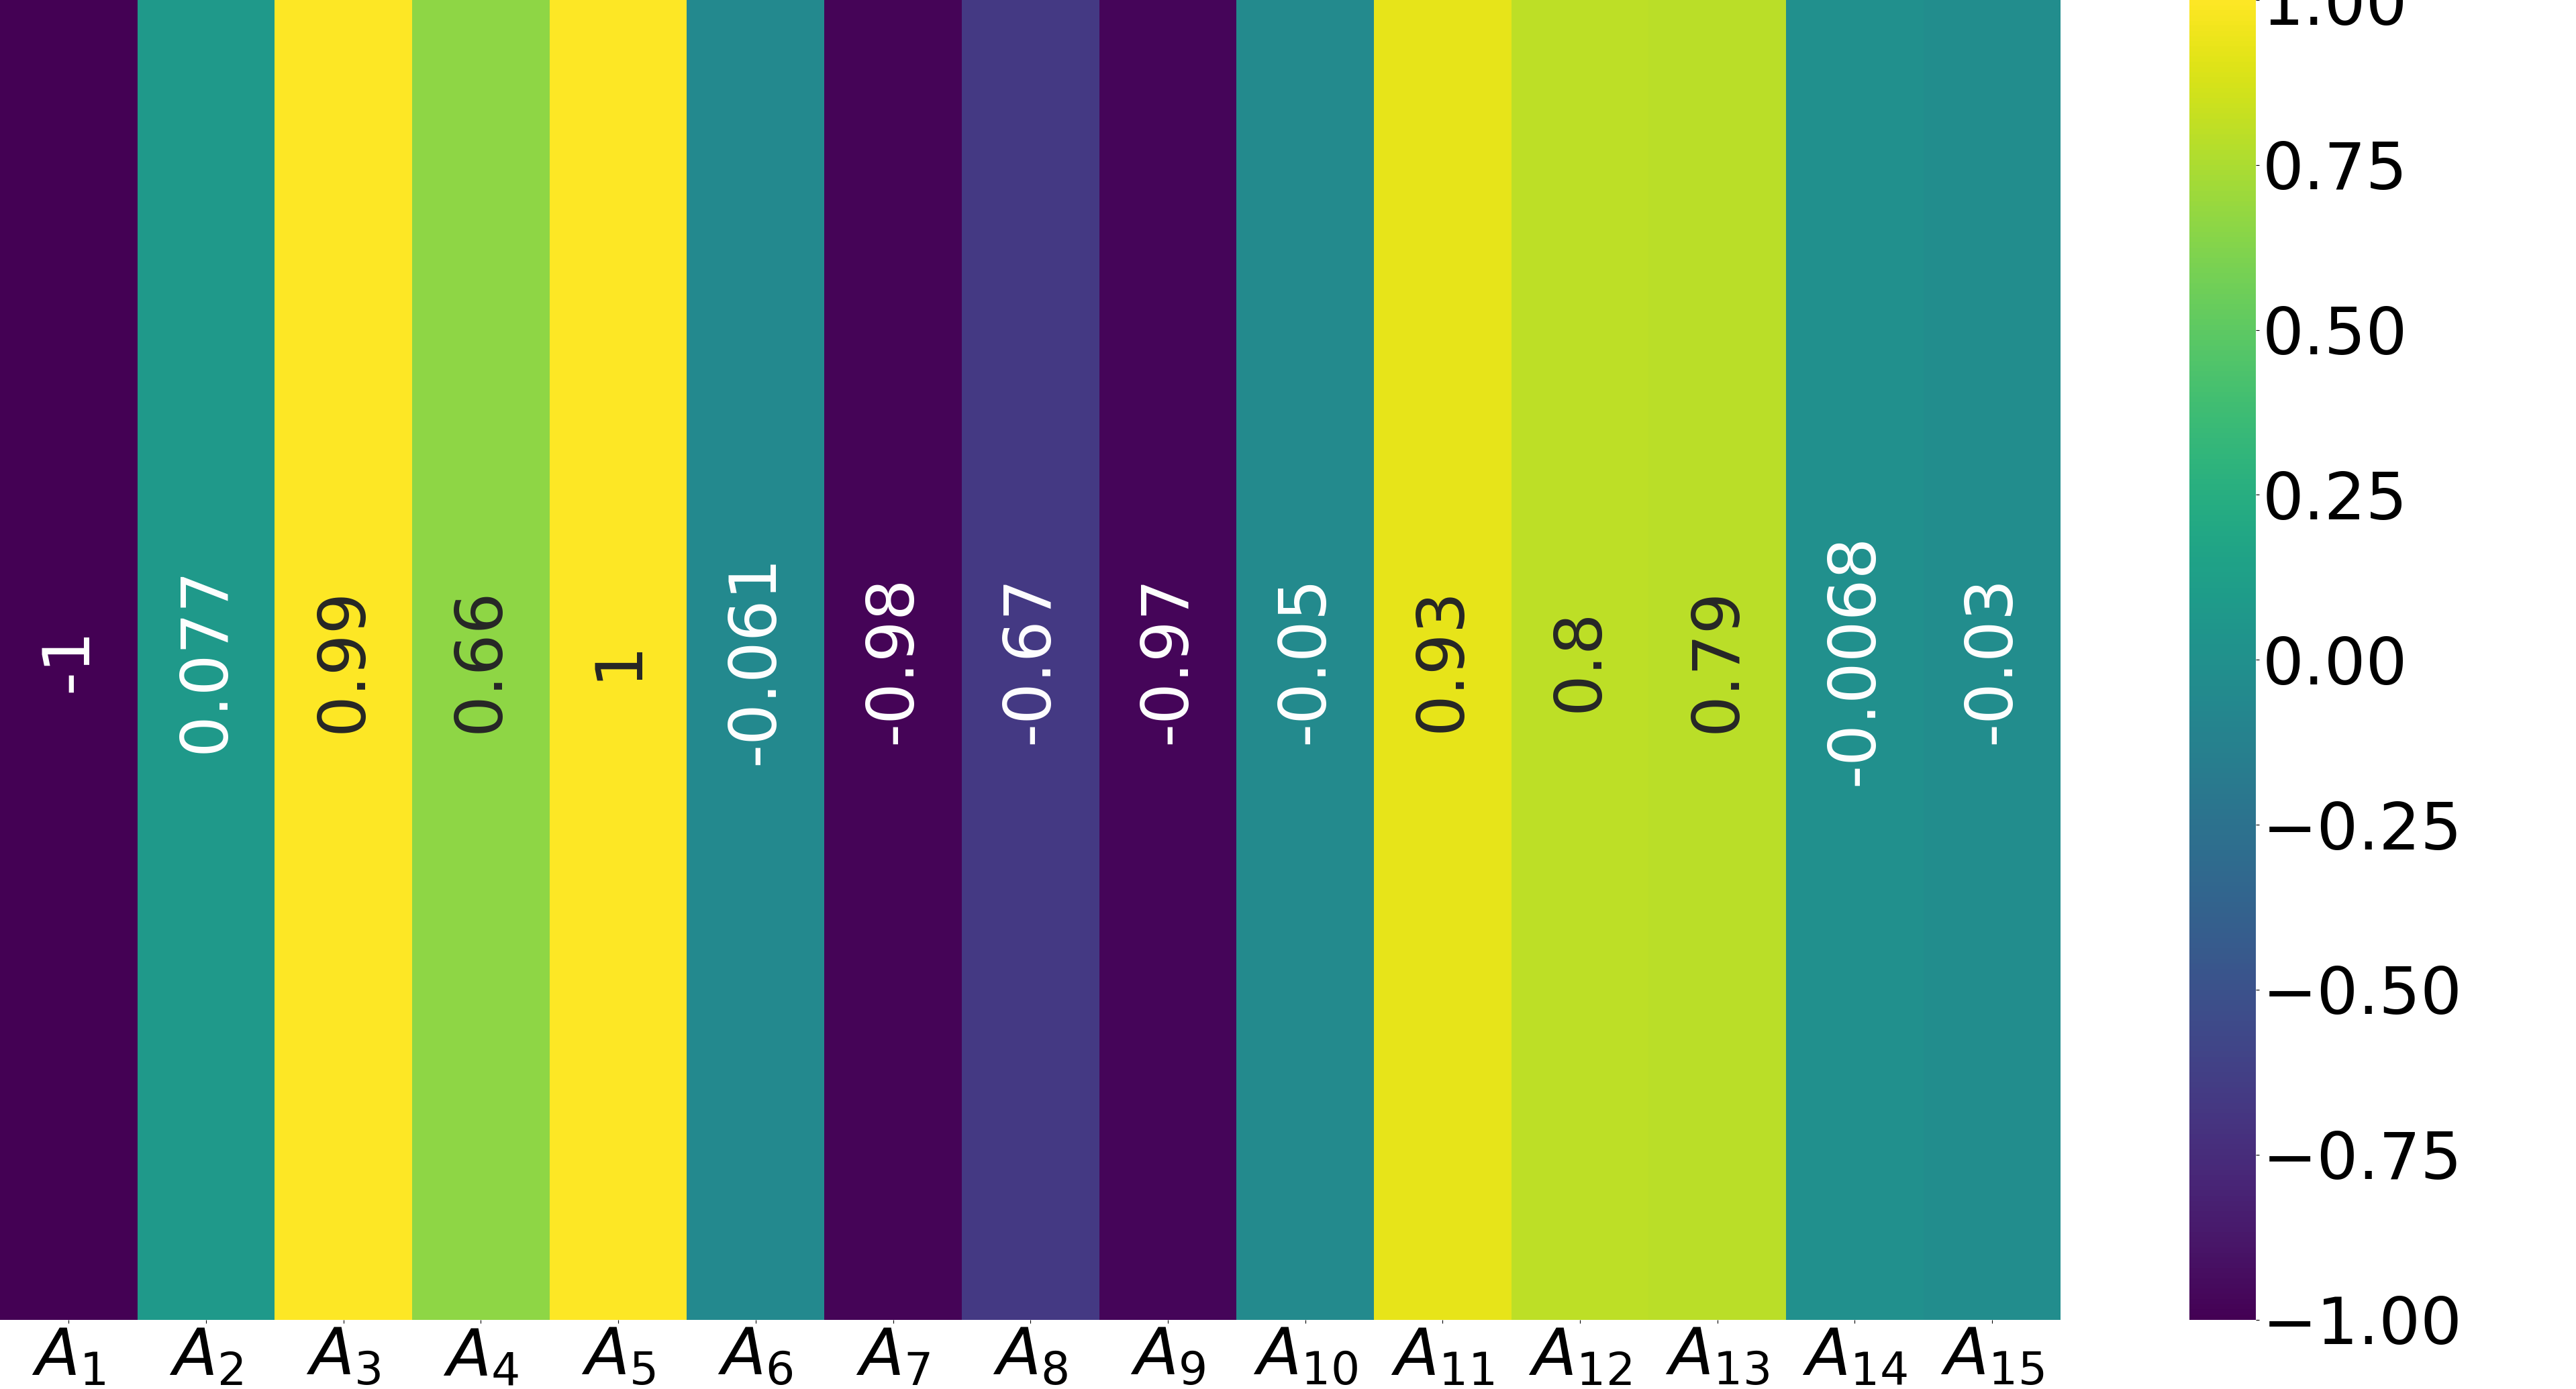
\includegraphics[width=\linewidth]{img/qlp_corr/An_coil0.png}
		\subcaption{Correlation with coil $0$}
	\end{subfigure}
	\begin{subfigure}{0.49\linewidth}
		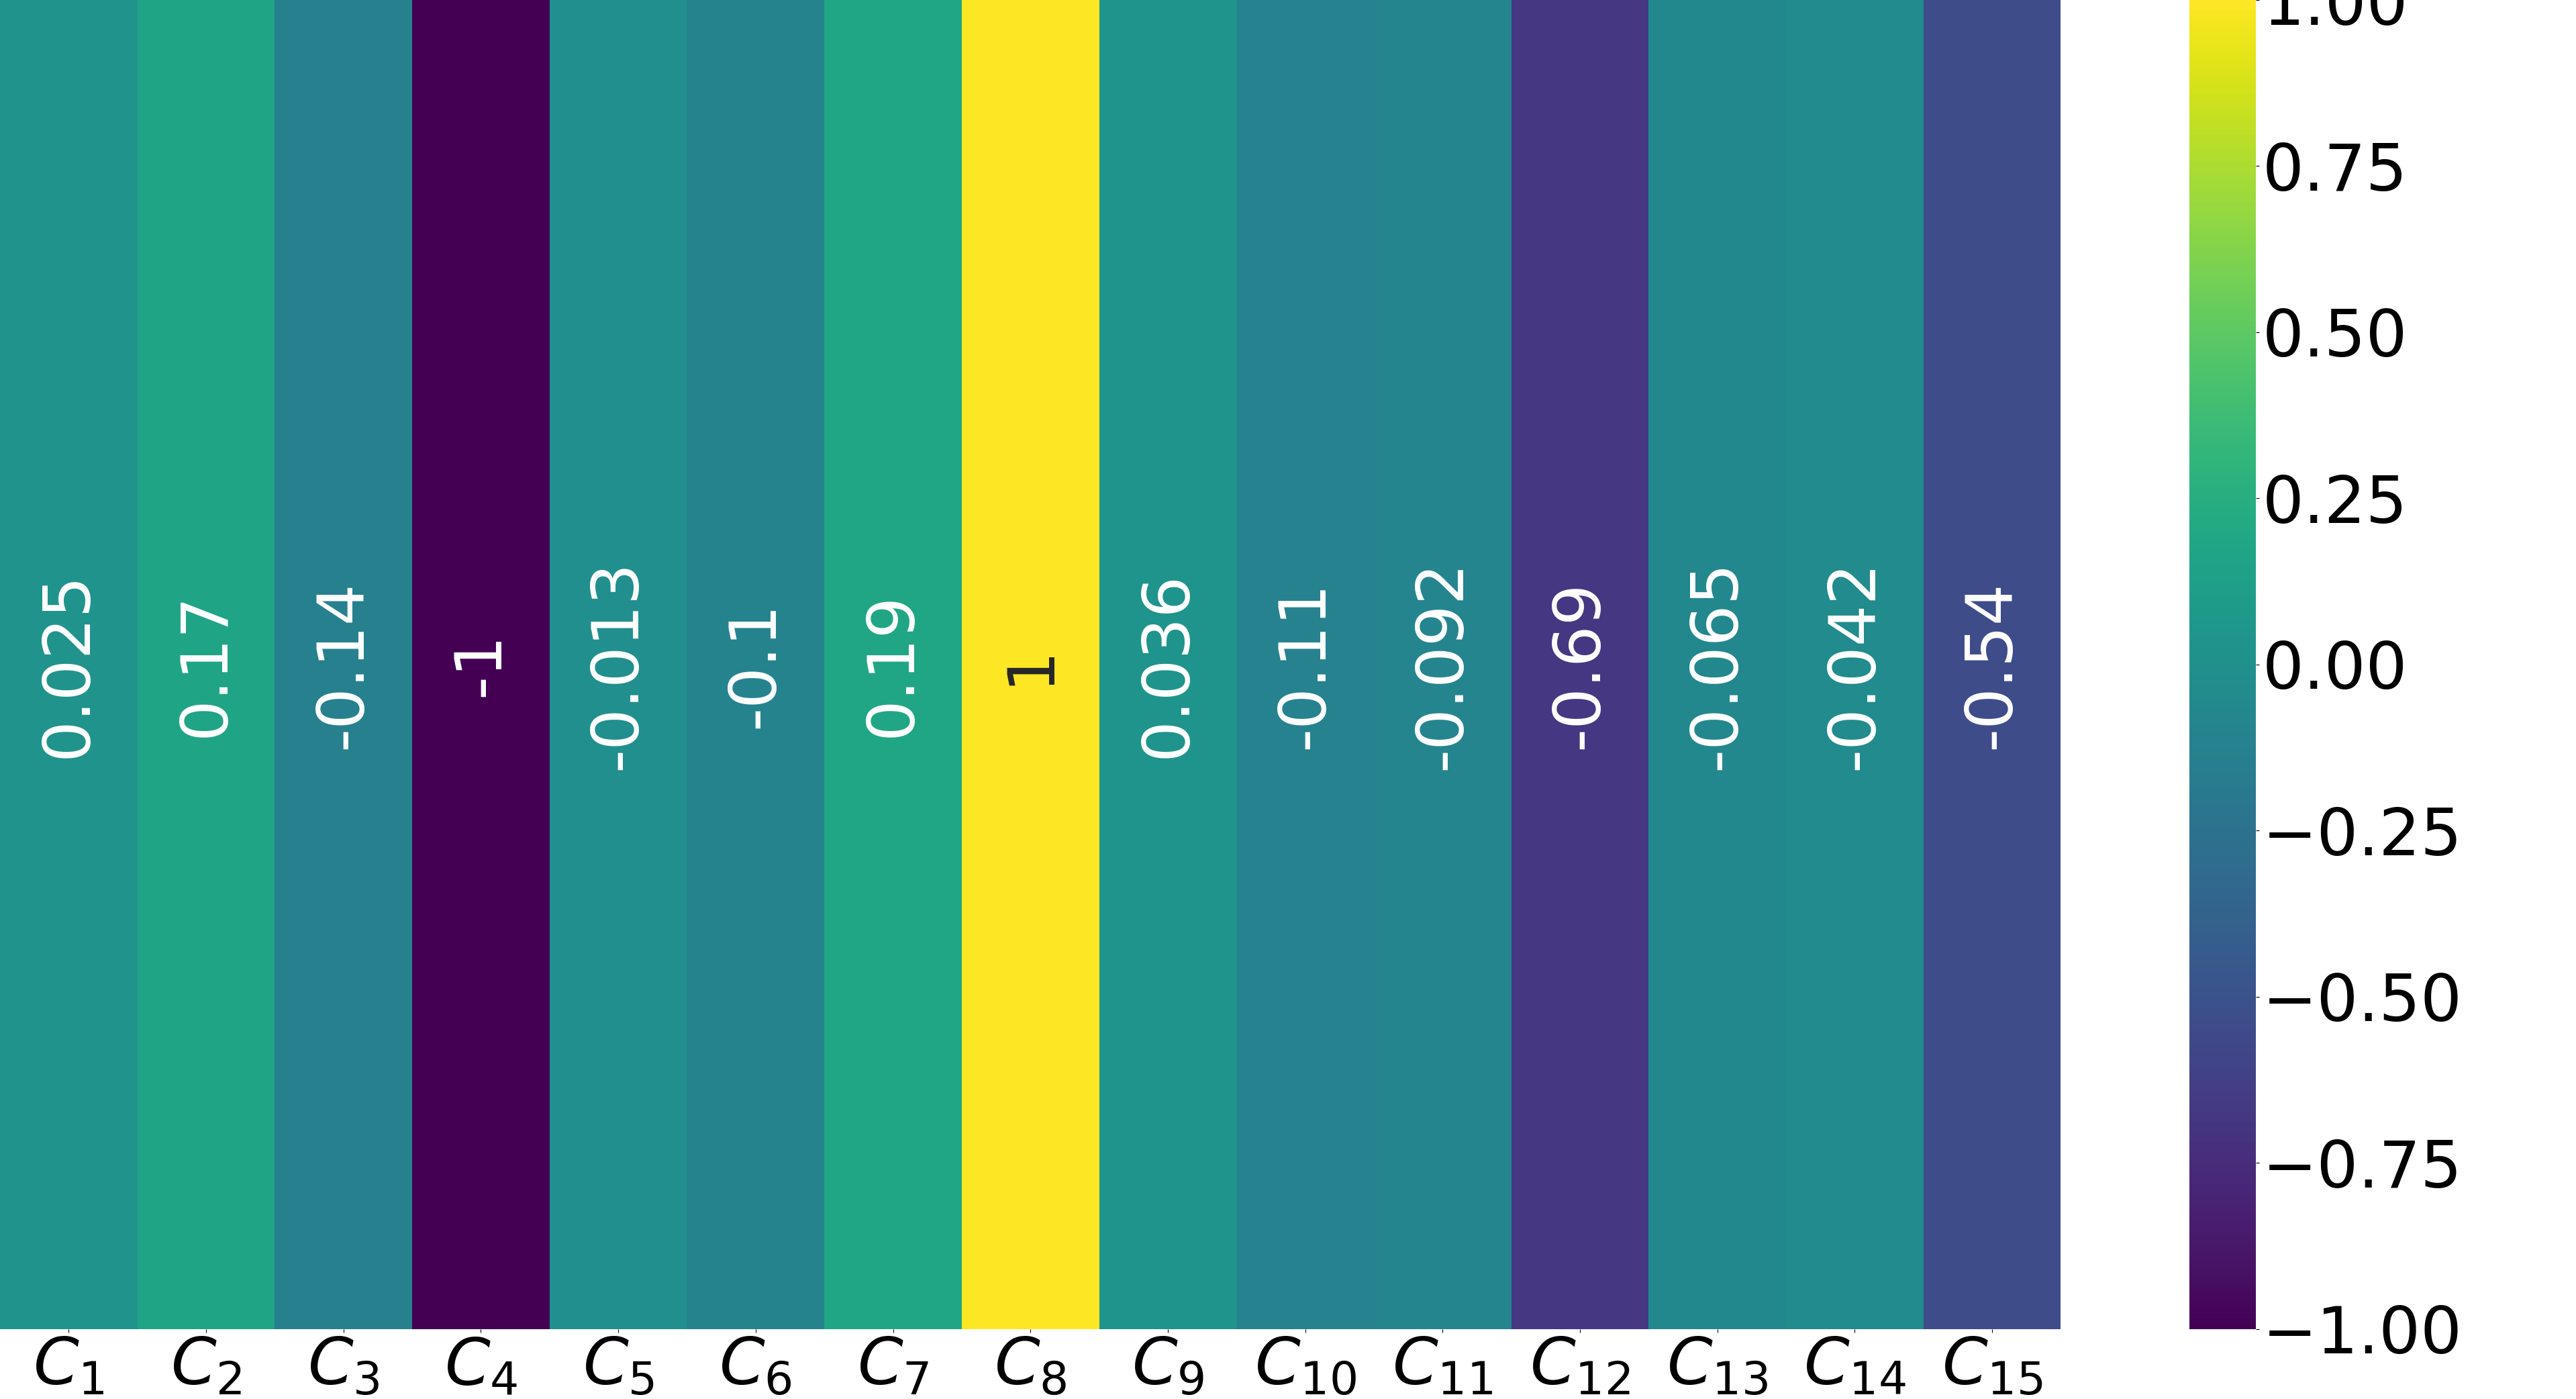
\includegraphics[width=\linewidth]{img/qlp_corr/An_coil1.png}
		\subcaption{Correlation with coil $1$}
	\end{subfigure}
	\begin{subfigure}{0.49\linewidth}
		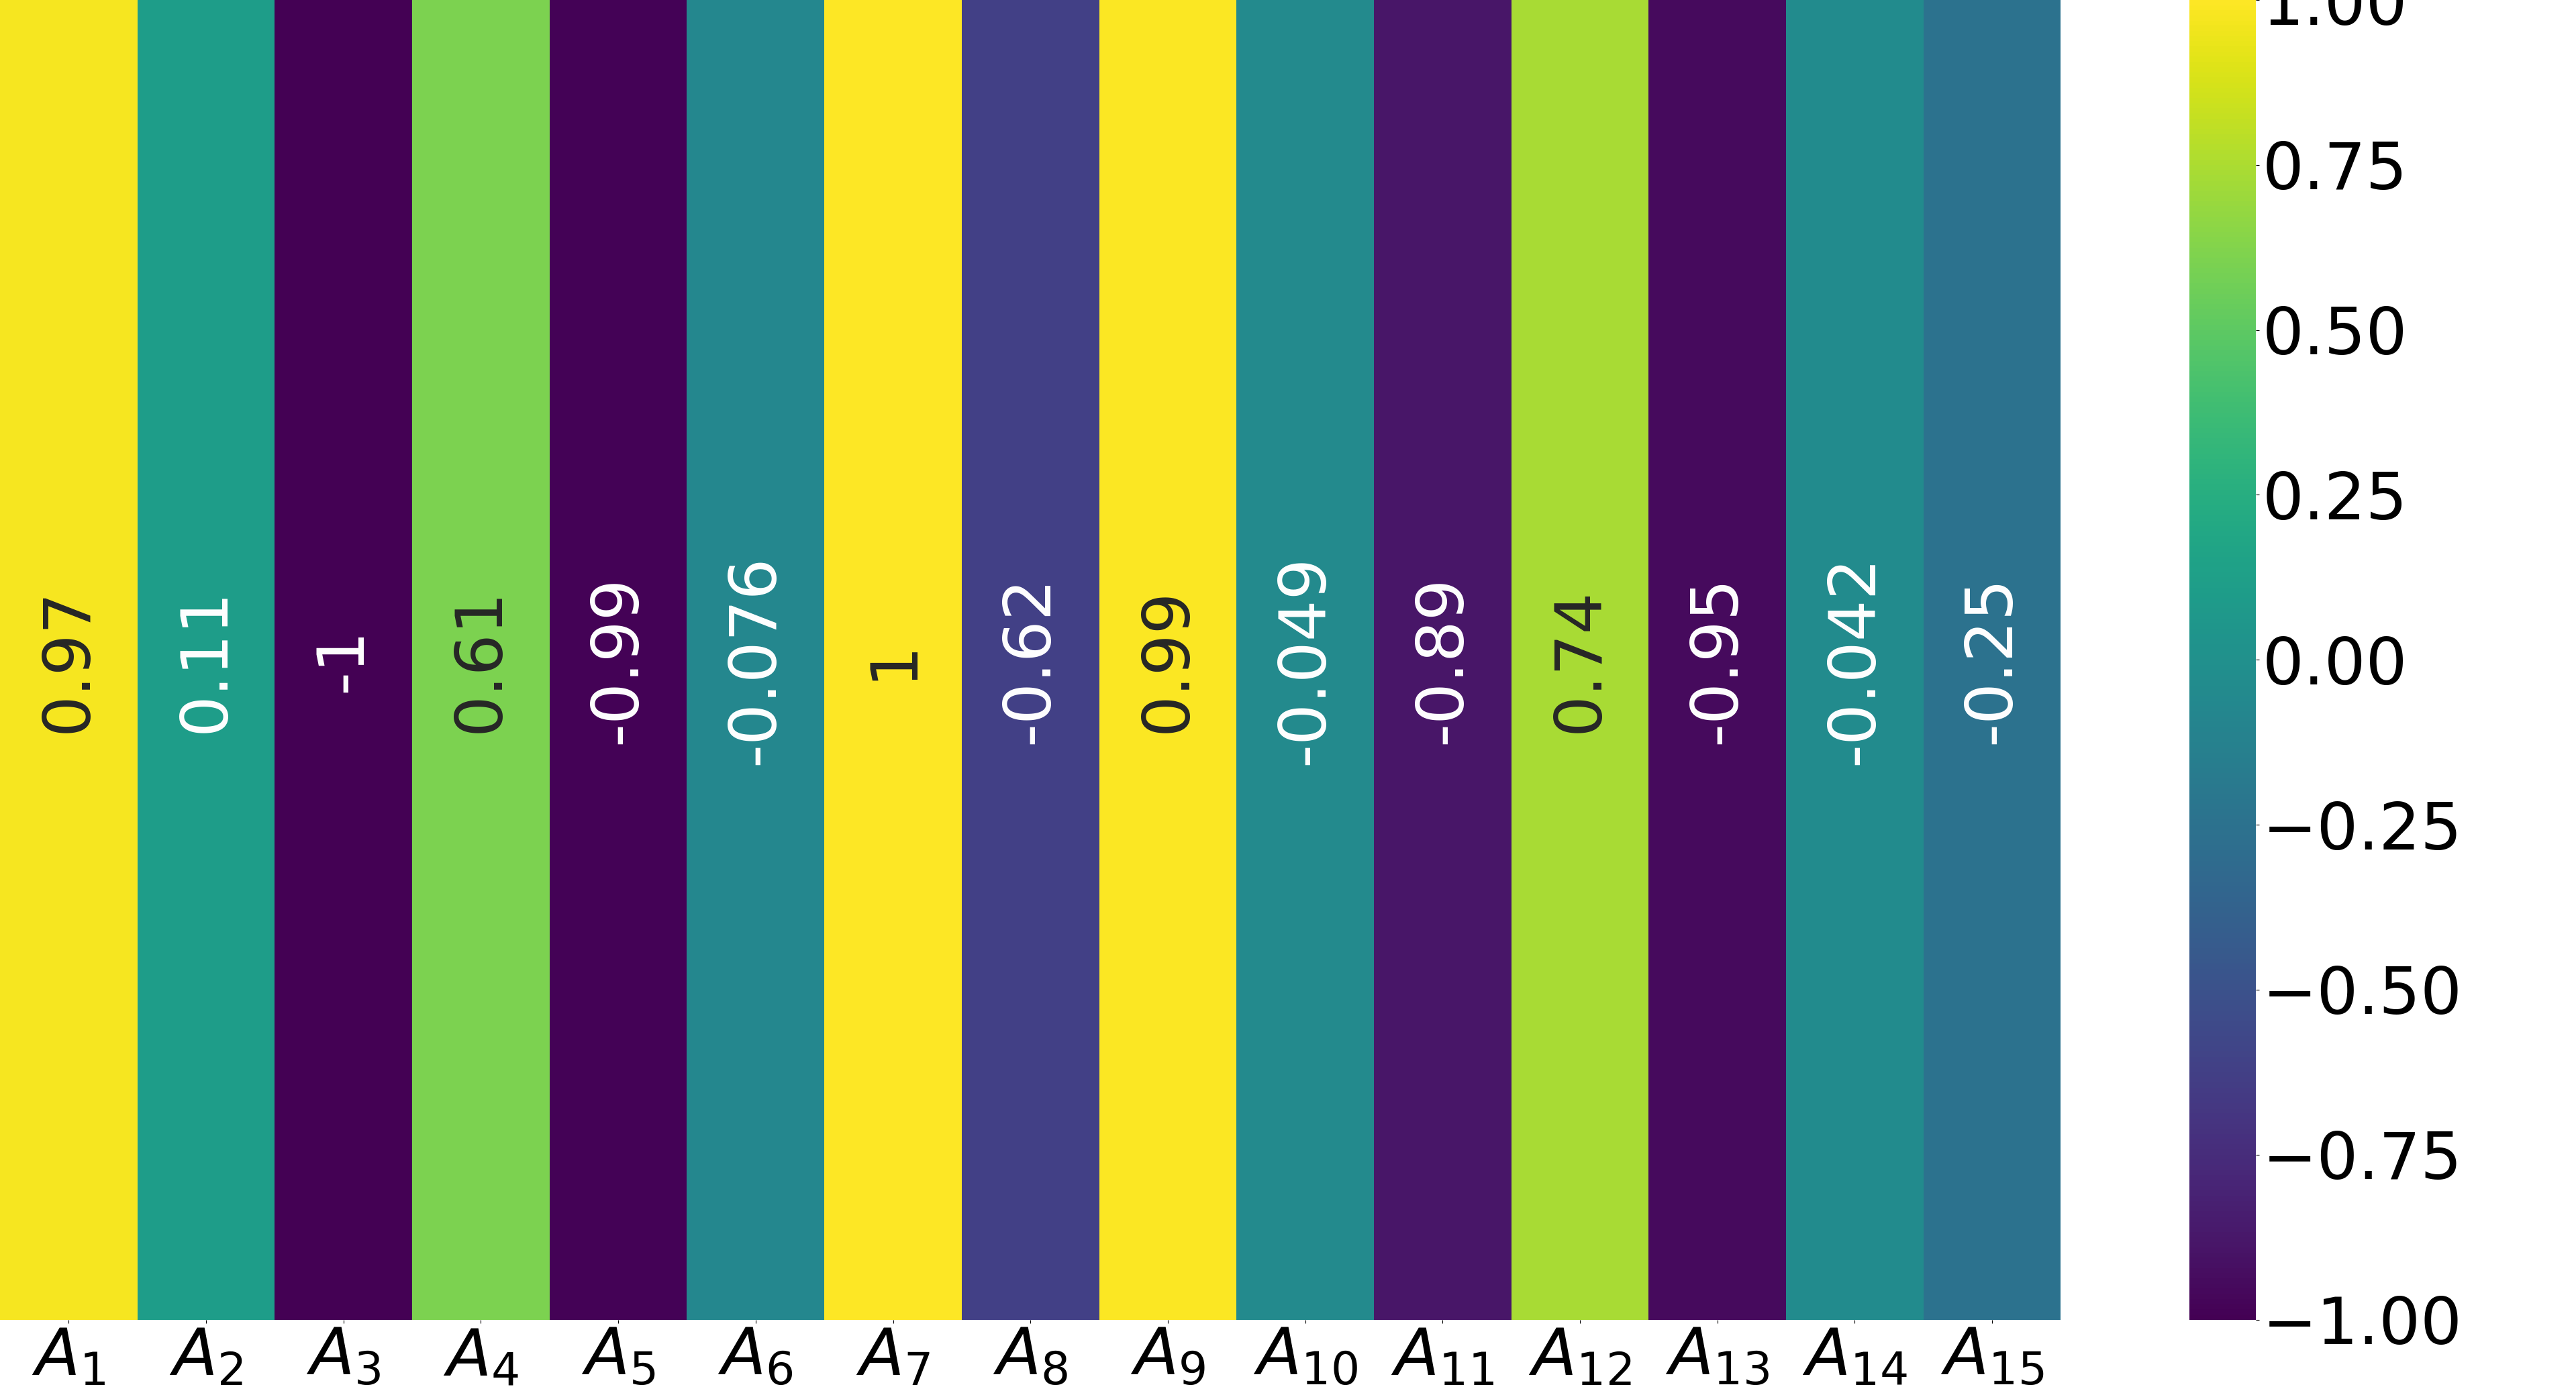
\includegraphics[width=\linewidth]{img/qlp_corr/An_coil2.png}
		\subcaption{Correlation with coil $2$}
	\end{subfigure}
	\begin{subfigure}{0.49\linewidth}
		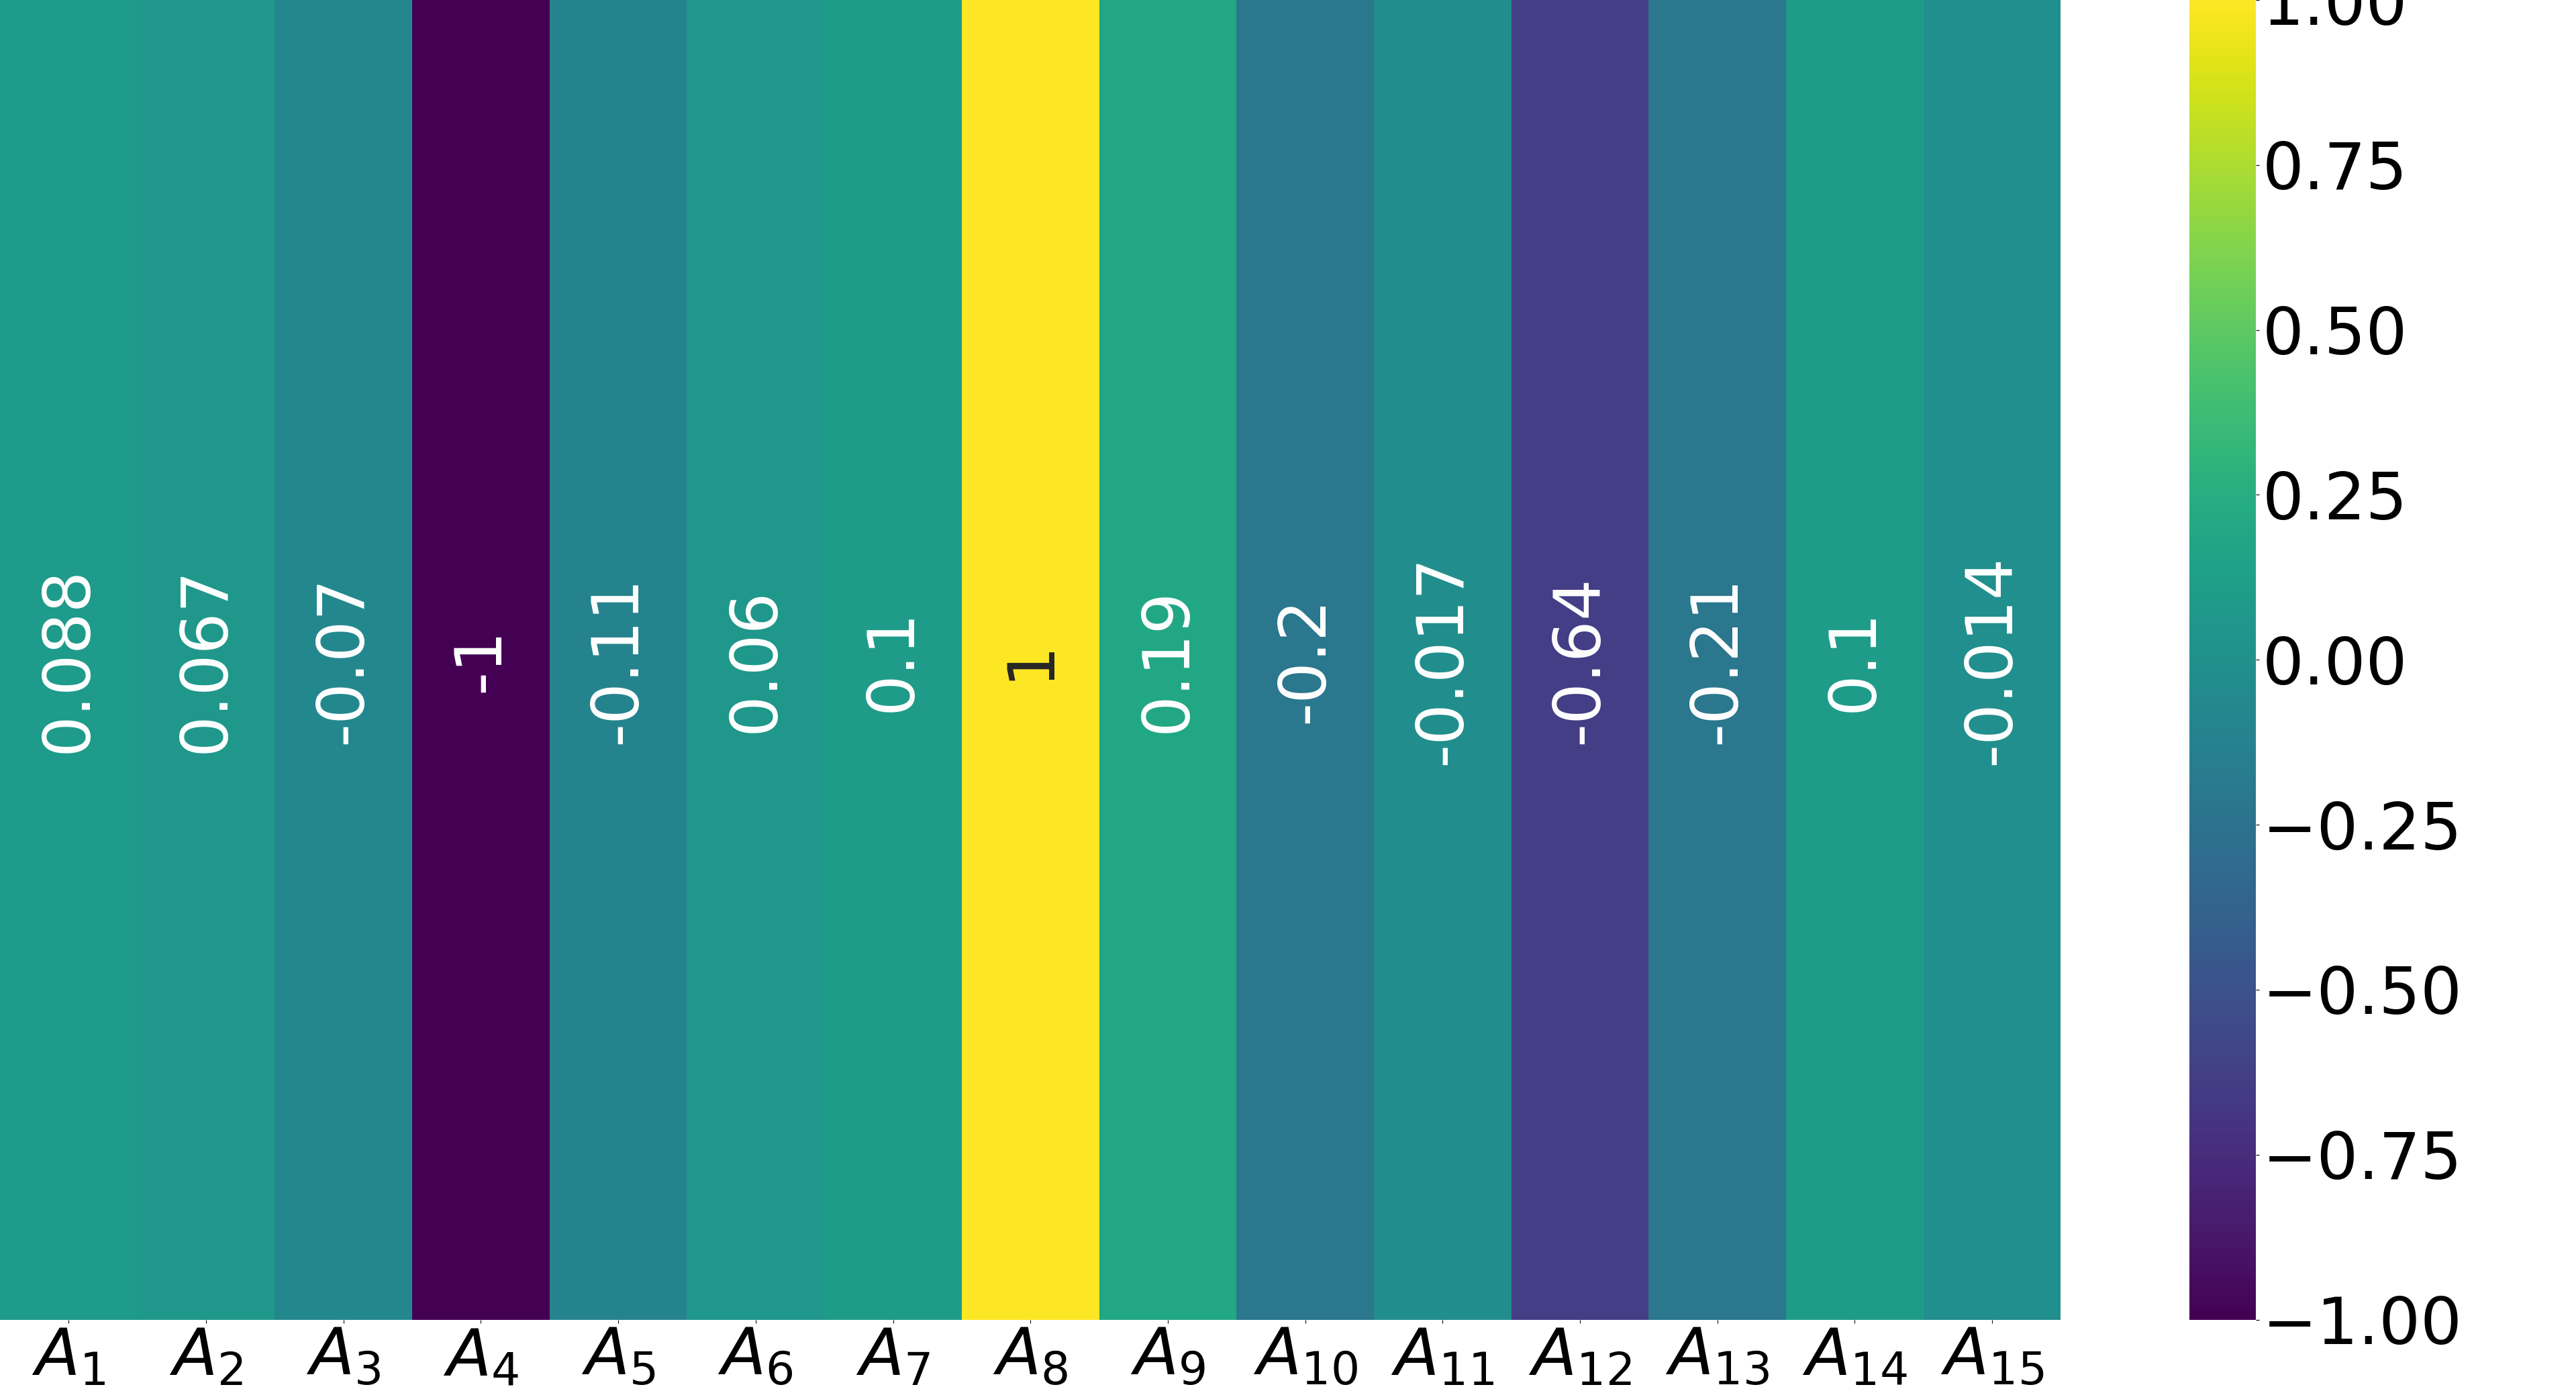
\includegraphics[width=\linewidth]{img/qlp_corr/An_coil3.png}
		\subcaption{Correlation with coil $3$}
	\end{subfigure}
	\caption{Correlation between the harmonics of the \an\ attribute and the labels for \qlp.}
	\label{fig:an-lcorr-qlp}
\end{figure}

In figure \Cref{fig:an-coilq-dist} we visualized the distribution of samples for \an\ in
bidimensional space, after a round of \pca\ dimensionality reduction (moving from $15$ to $2$
dimensions). Sub-figure (a) labels data based on the number of quenched coils associated to the
sample. We can evidently identify a series of clusters, characterized by a high degree of purity, in
\Cref{sec:qlp-cluster} we are going to discuss the clustering approach on this specific attribute.
In sub-figure (b), we labelled the data based on which coil was quenched. The division of the labels
is not as neat as in sub-figure (a), which lead us to think that clustering could be used as a
preprocessing step to then have another machine learning model work on the clustered data to
predict quench localization.

While sub-figure (b) doesn't tell us everything we need to know, we can see that coil $1$ and coil
$3$ are fairly mixed together, furthermore both of them are usually involved in multi-coil quenches.
These hints are giving us another possible reason why the attribute is less-than-ideal to
predict quench localization on coils $3$ and $1$ \Cref{fig:an-lcorr-qlp}.

\begin{figure}[!ht]
	% Font size = 40
	\centering
	\begin{subfigure}{0.8\linewidth}
		\centering
		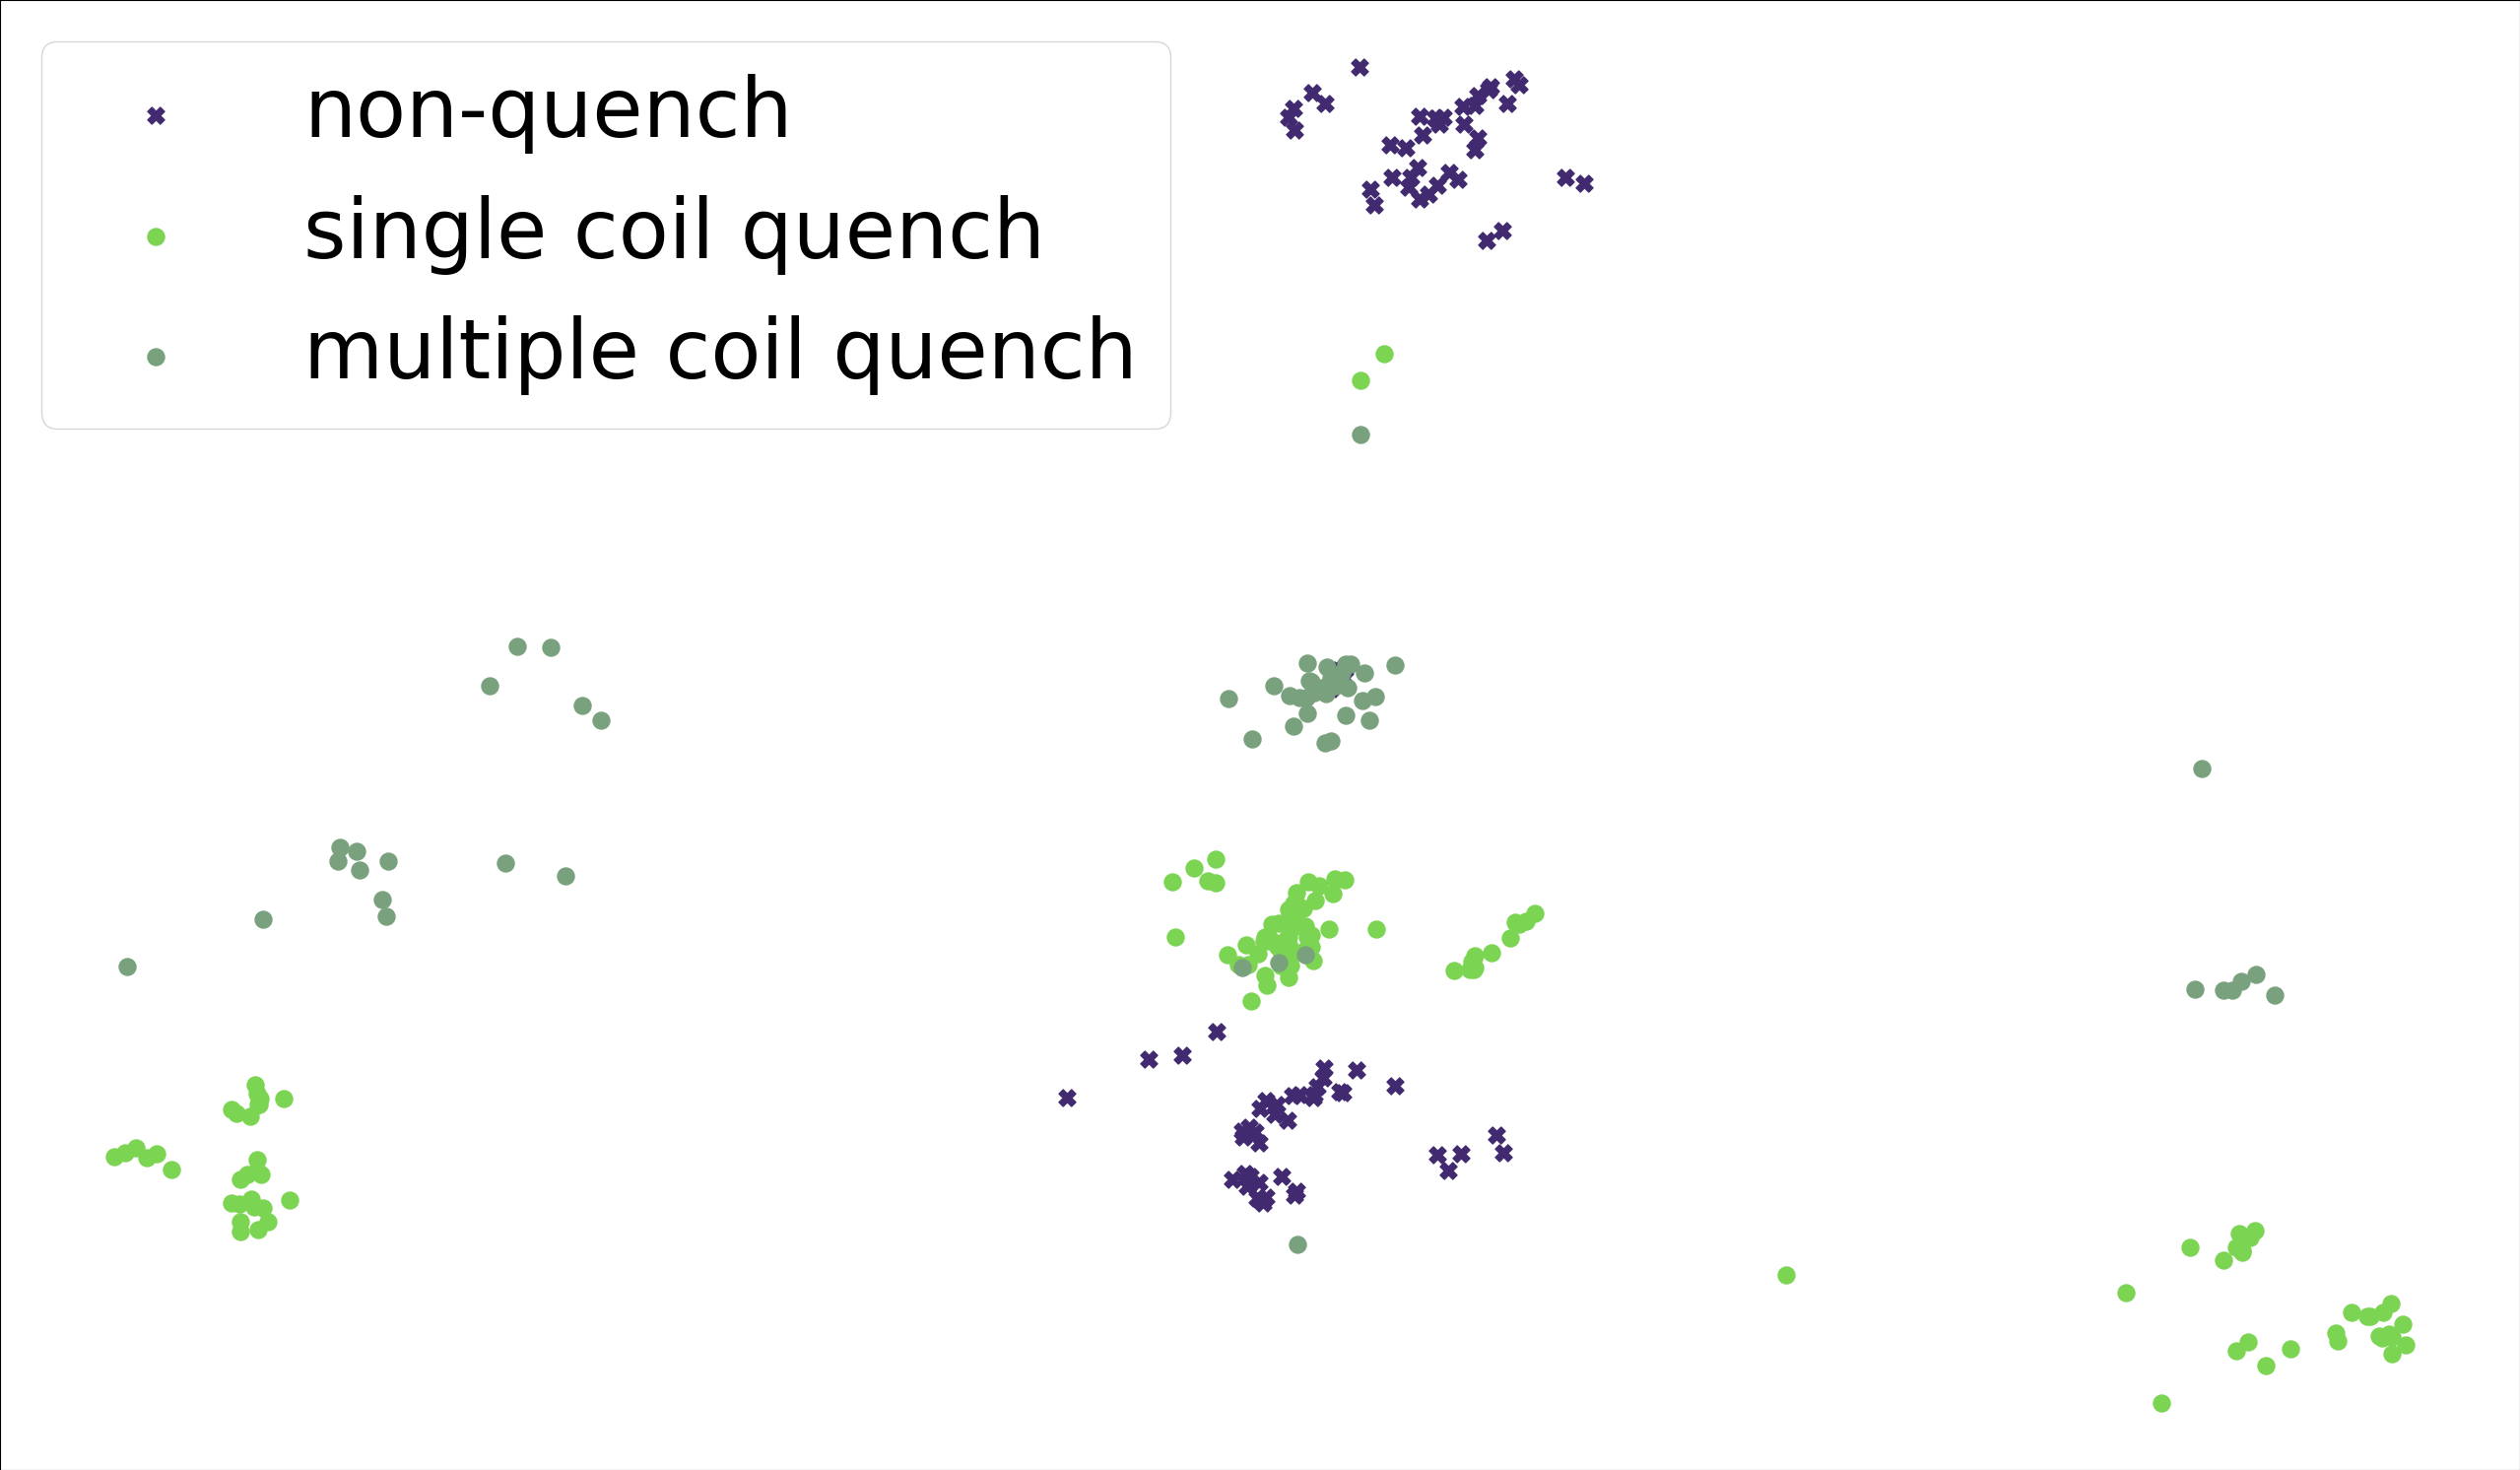
\includegraphics[width=\linewidth]{img/quench_dist_qlp/single_vs_multiple_An.png}
		\subcaption{}
	\end{subfigure}
	\begin{subfigure}{0.8\linewidth}
		\centering
		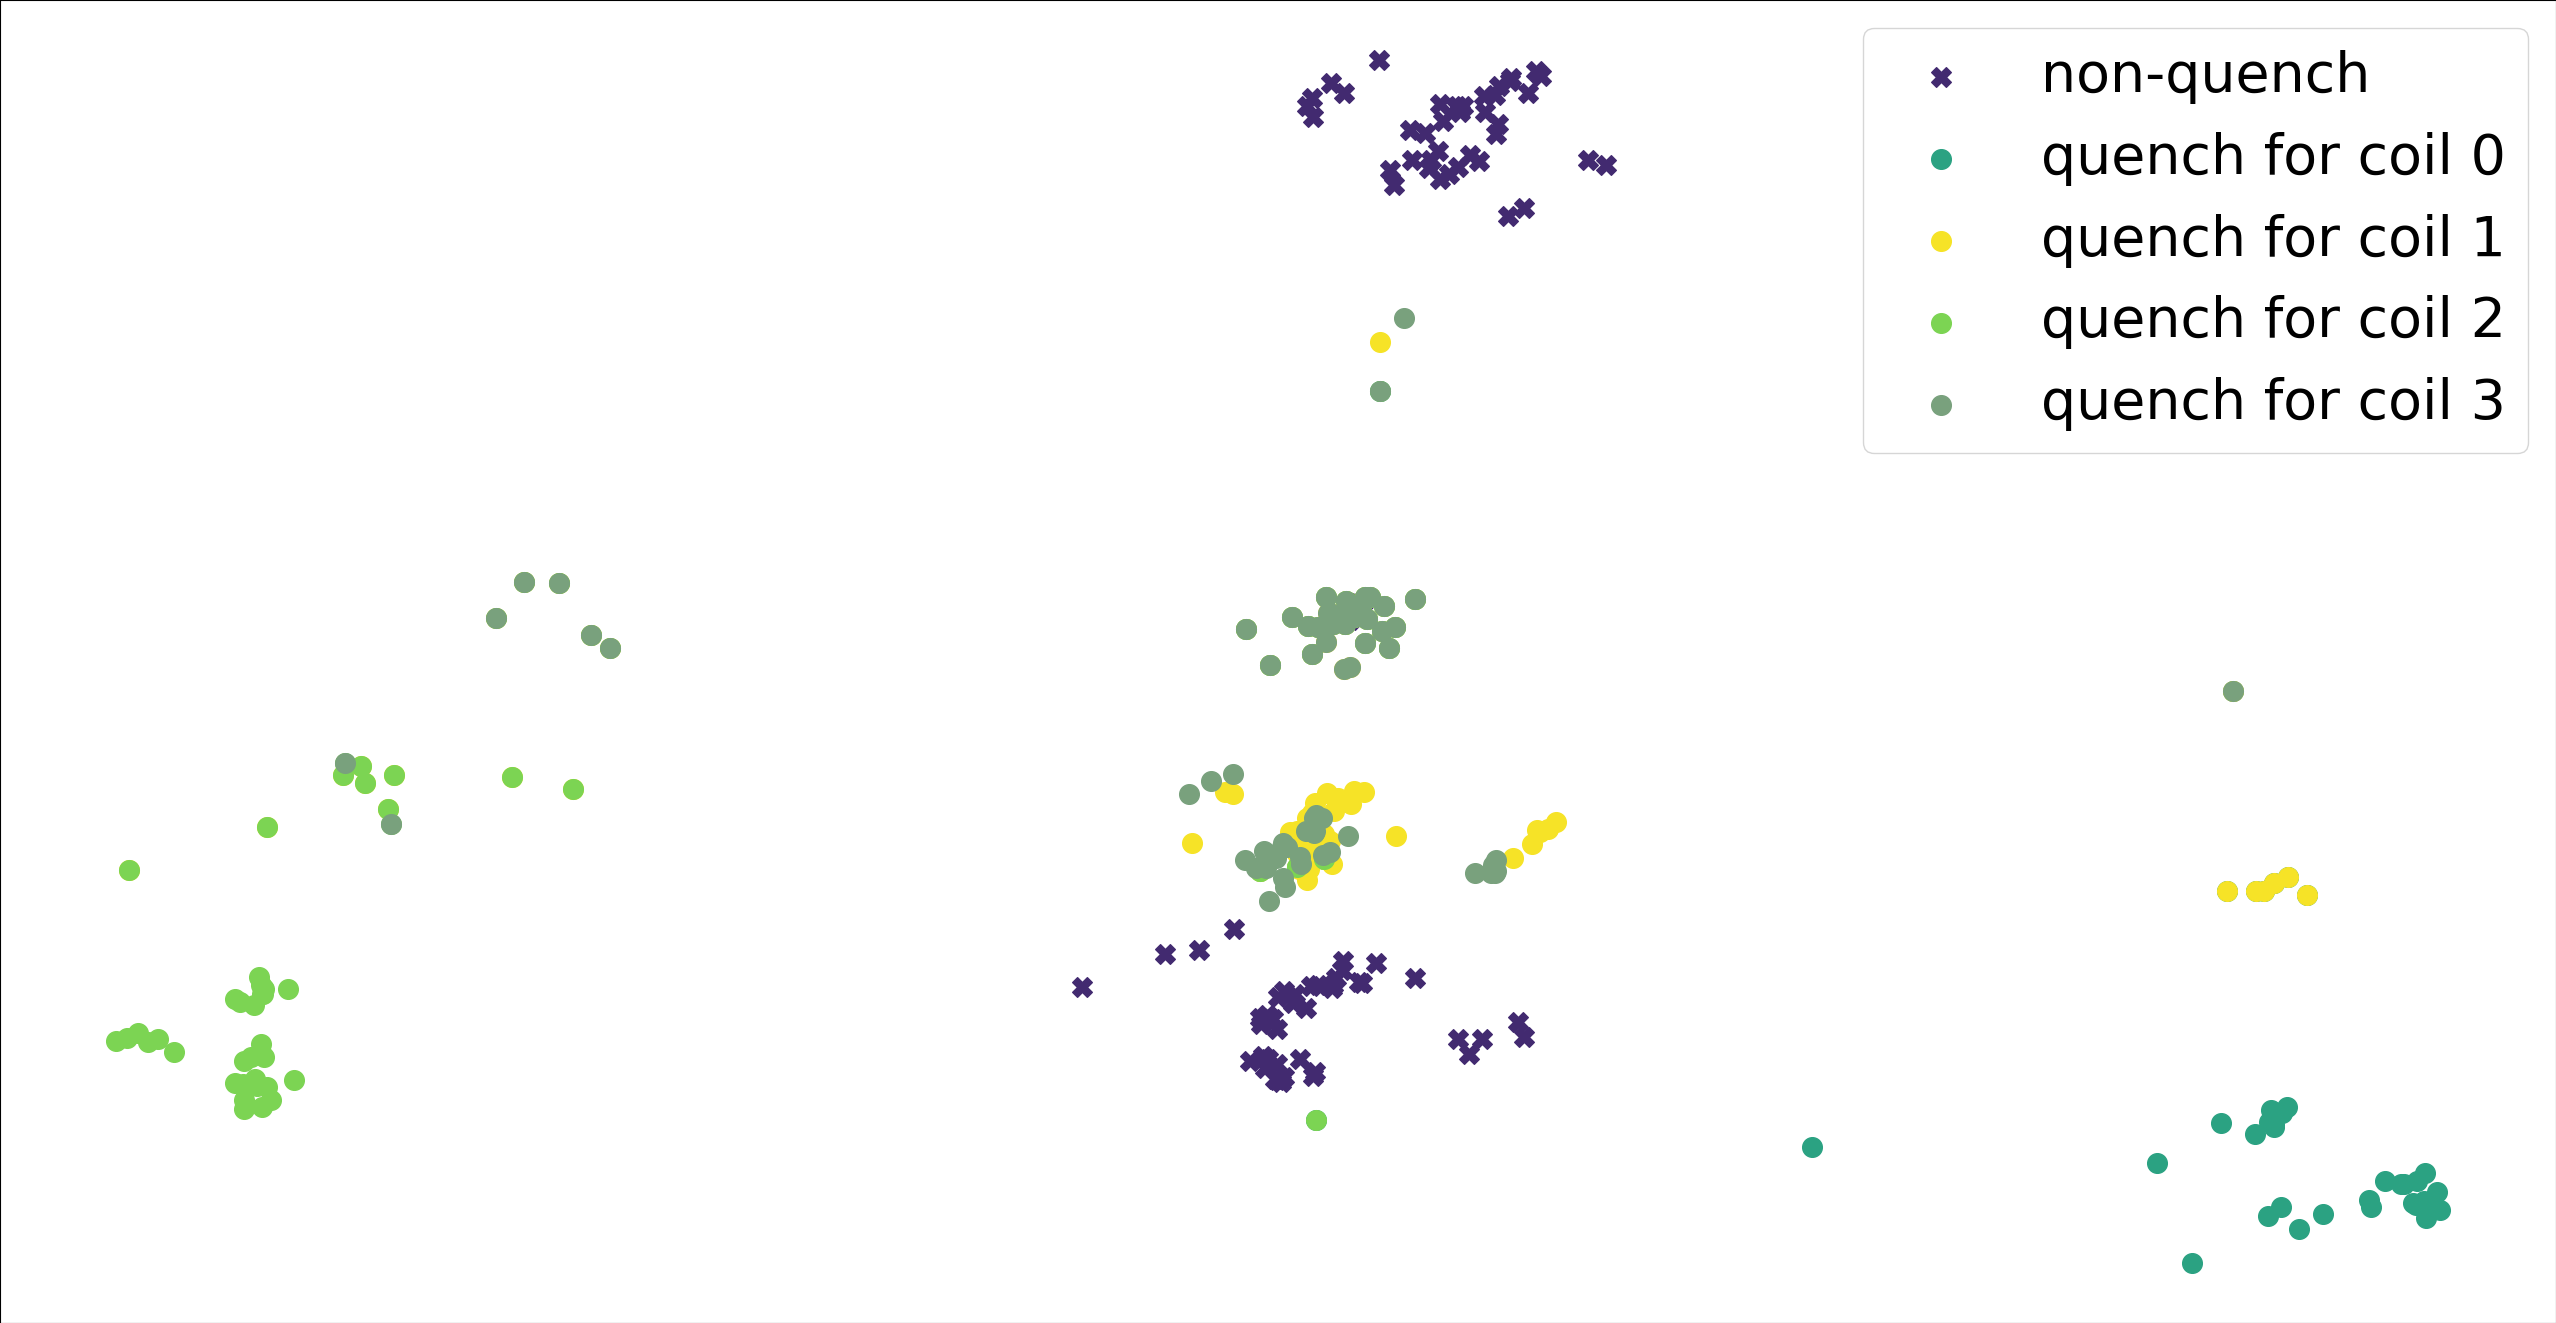
\includegraphics[width=\linewidth]{img/quench_dist_qlp_an.png}
		\subcaption{}
	\end{subfigure}
	\caption{Visualization of the \an\ attribute, the data was plotted after a run of \pca\
		dimensionality reduction. Sub-figure (a) highlights the samples based on how many quenches
		are associated to the specific sample $\{0, 1, \text{many}\}$. Sub-figure (b) highlights the
		samples based on the specific coil quenched $\{\text{None}, 0, 1, 2, 3\}$.}\label{fig:an-coilq-dist}
\end{figure}

\subsubsection{\bn}
While experimenting with \qrp, we discovered that \bn\ was the attribute that performed the least
among the ones available. We expected similar results for \qlp, but from preprocessing alone we
could not understand whether the attribute promised good or bad performance.

\Cref{fig:bn-lcorr-qlp} highlights the correlation between \bn\ harmonics and the label associated
to each coil (as described in \Cref{chp:problem}). The attribute, similarly to \an, sees a pattern
of strong correlations between its odd-numbered harmonics and coils $1$ and $3$. Since the pattern
of sub-figures (b) and (d) is very similar to the one shown in sub-figures (a) and (c) of
\Cref{fig:an-lcorr-qlp}, we imagined that a plausible dataset composition would have followed rules
similar to the ones identified for \an.
\begin{figure}[!ht]
	% Font size = 70
	\centering
	\begin{subfigure}{0.49\linewidth}
		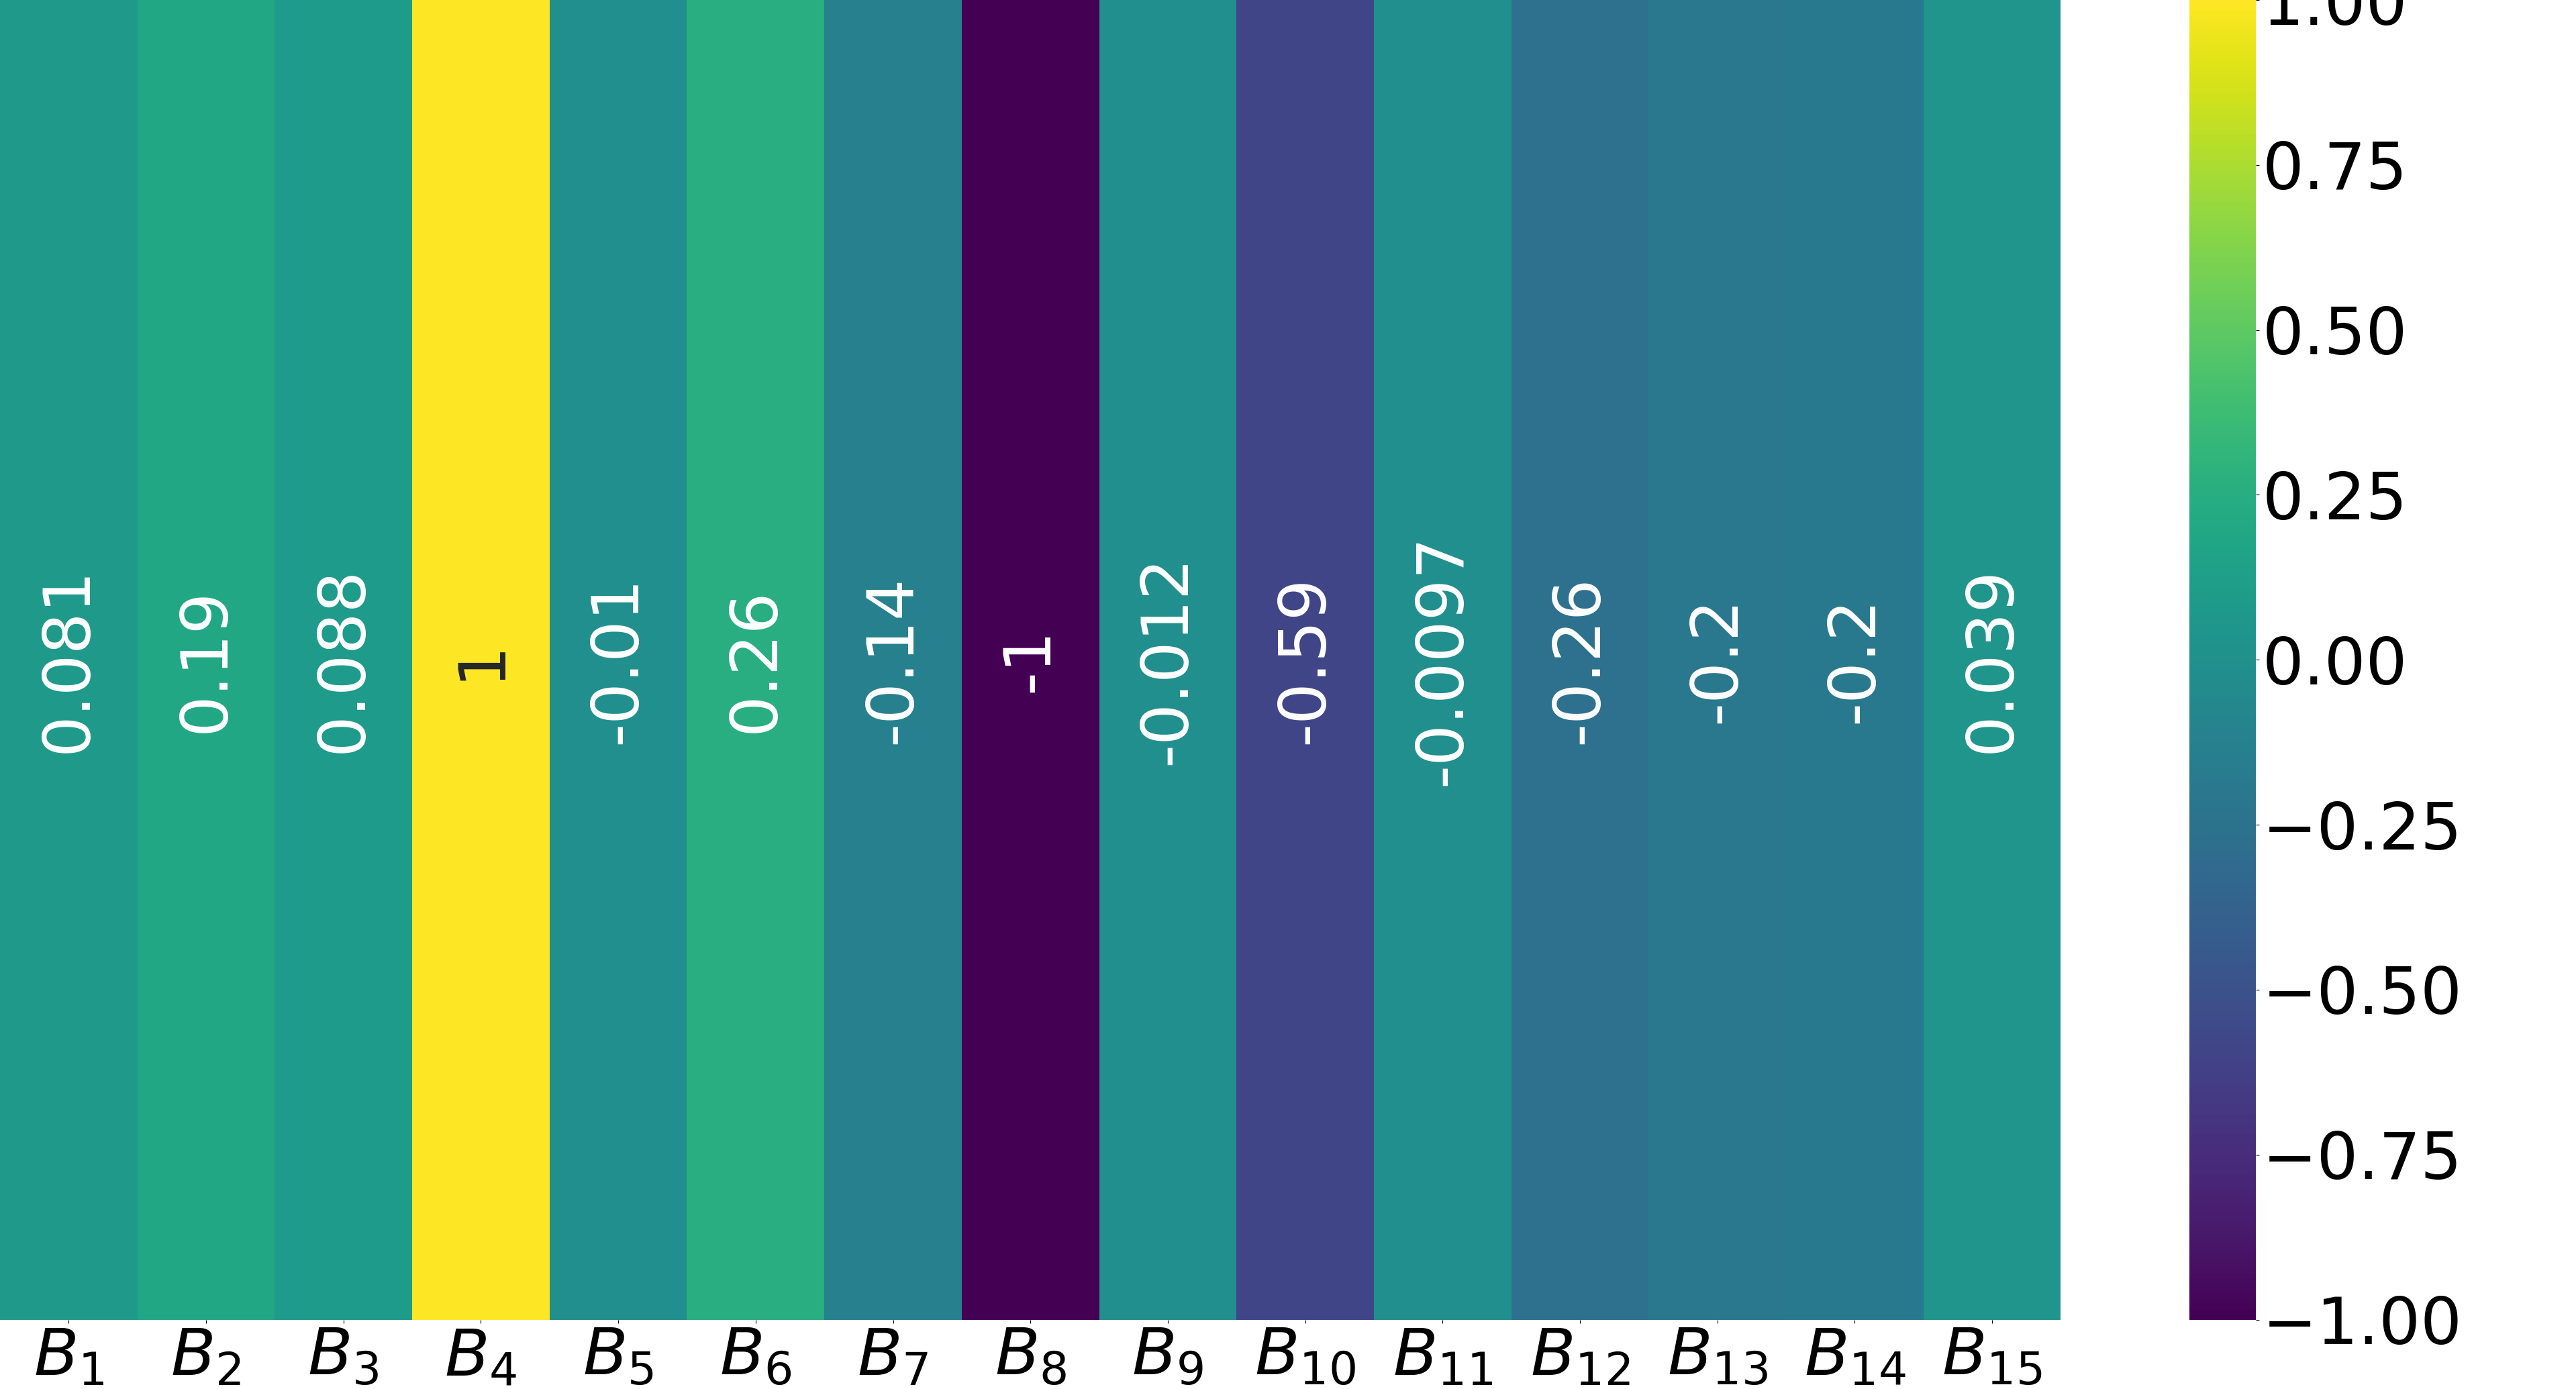
\includegraphics[width=\linewidth]{img/qlp_corr/Bn_coil0.png}
		\subcaption{Correlation with coil $0$}
	\end{subfigure}
	\begin{subfigure}{0.49\linewidth}
		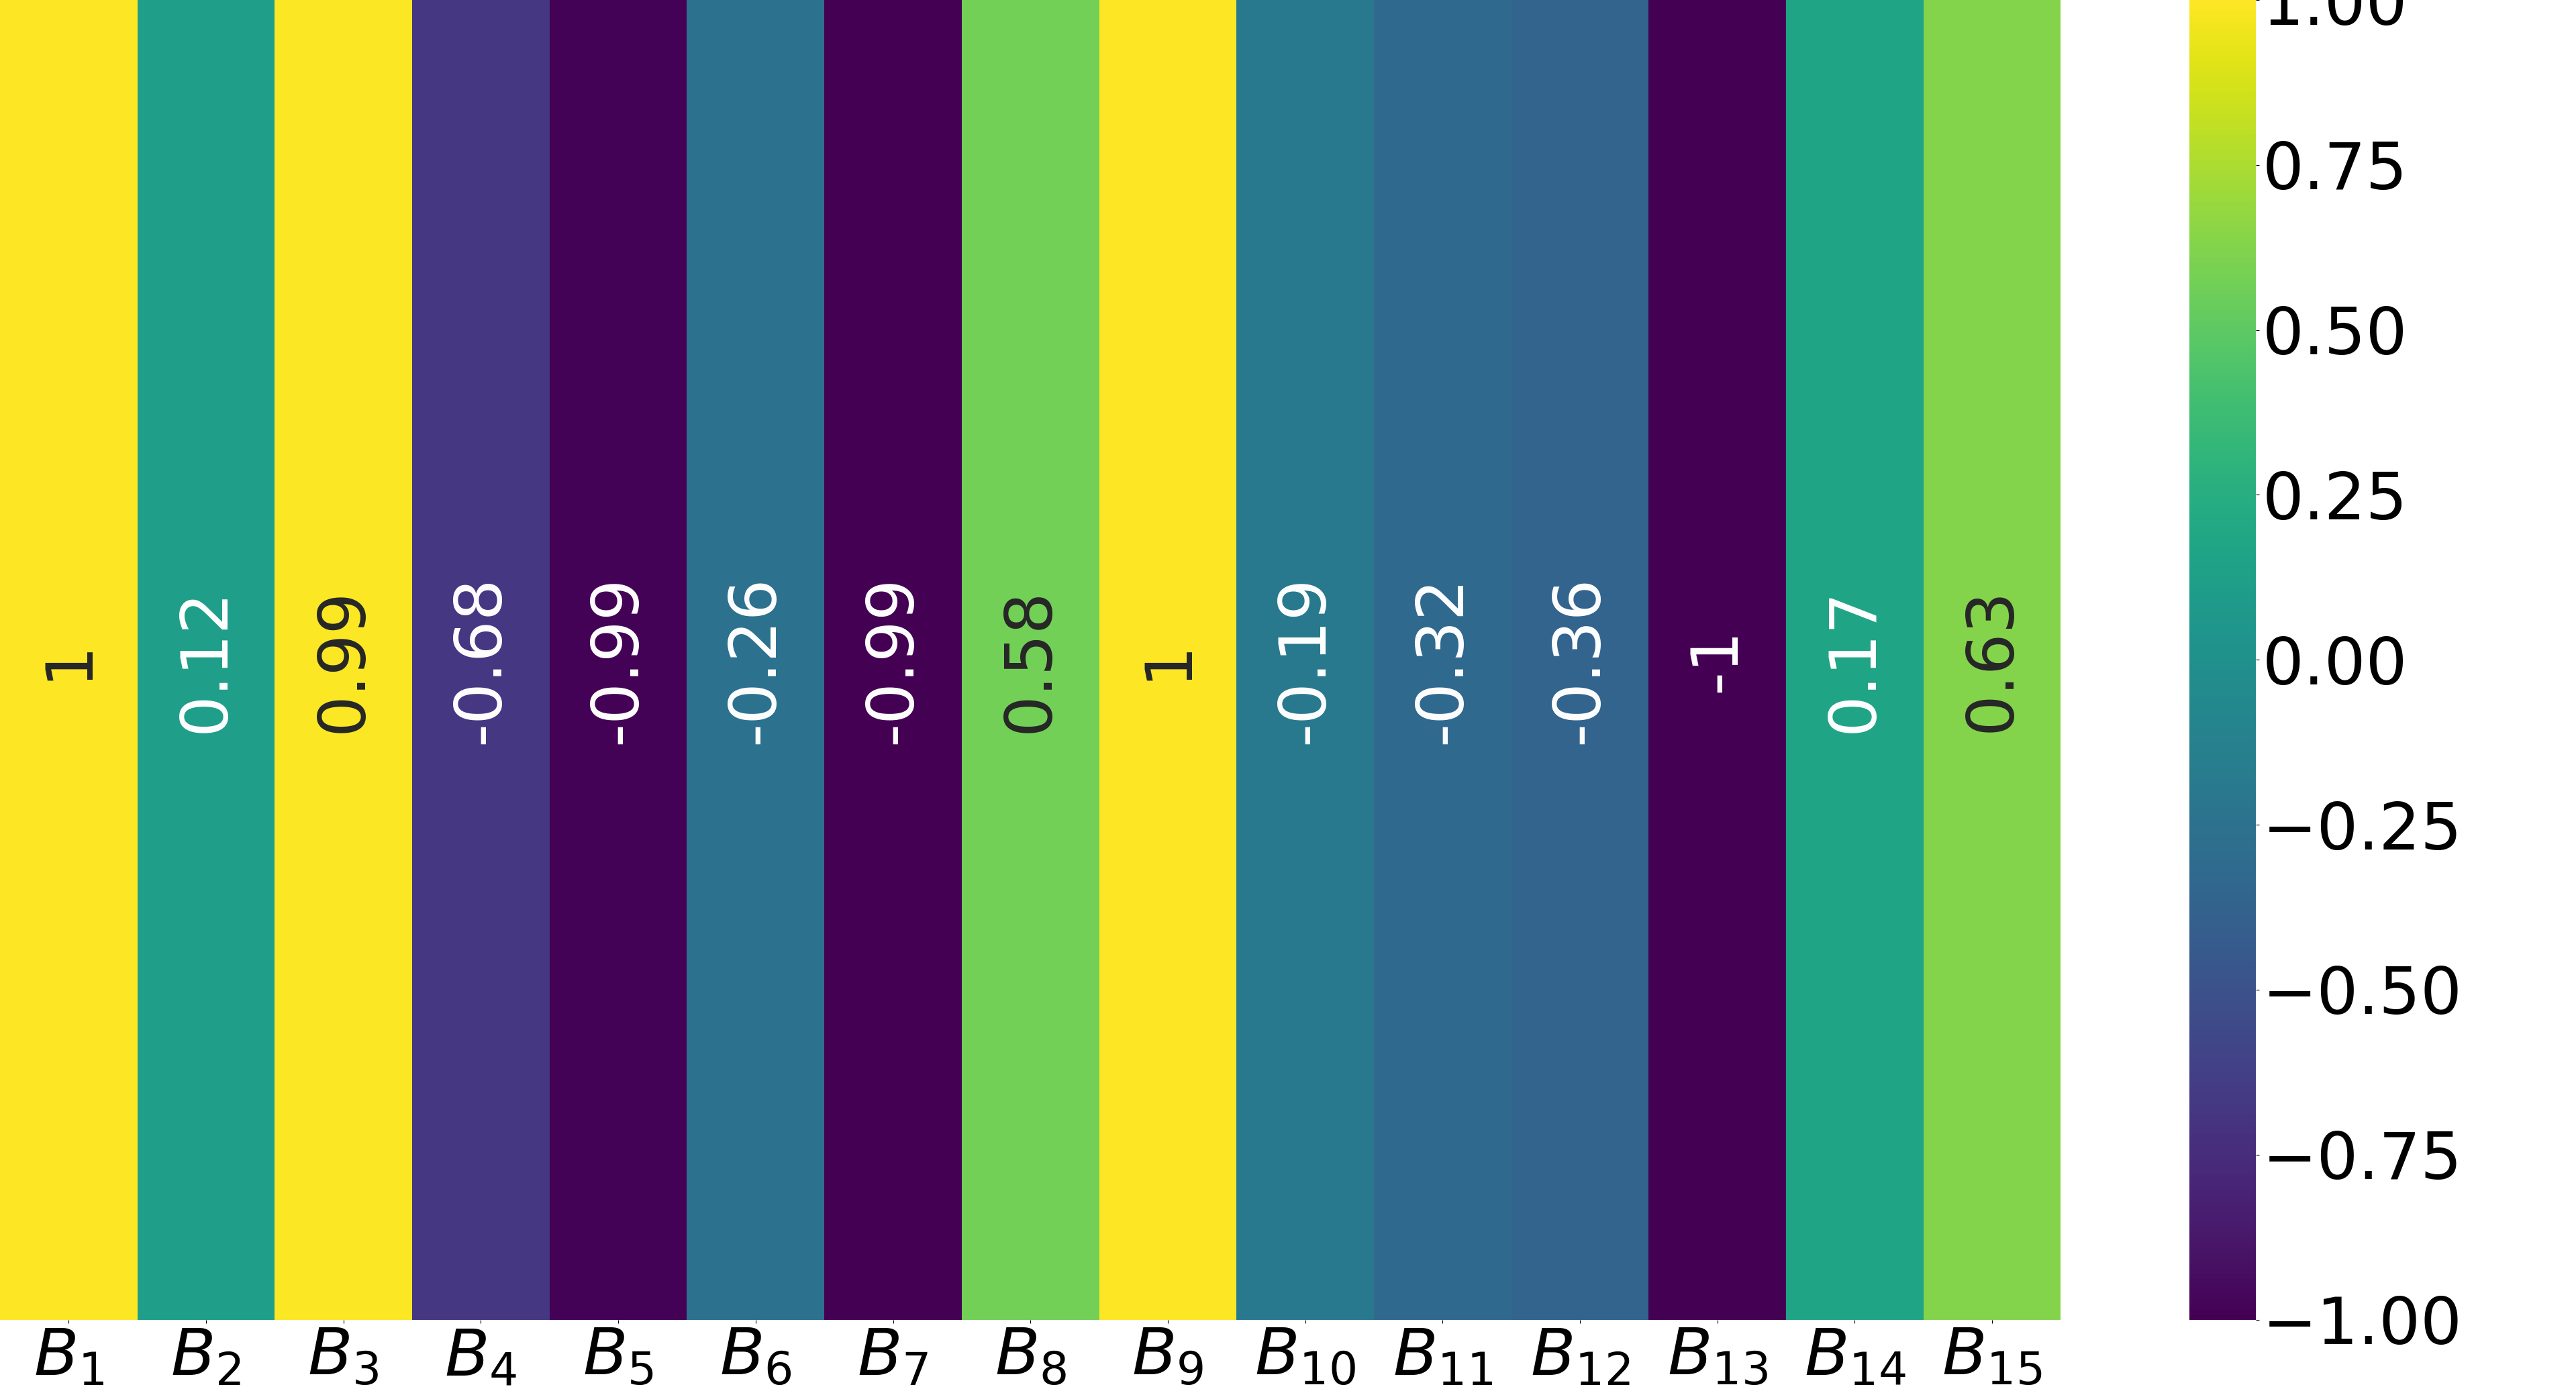
\includegraphics[width=\linewidth]{img/qlp_corr/Bn_coil1.png}
		\subcaption{Correlation with coil $1$}
	\end{subfigure}
	\begin{subfigure}{0.49\linewidth}
		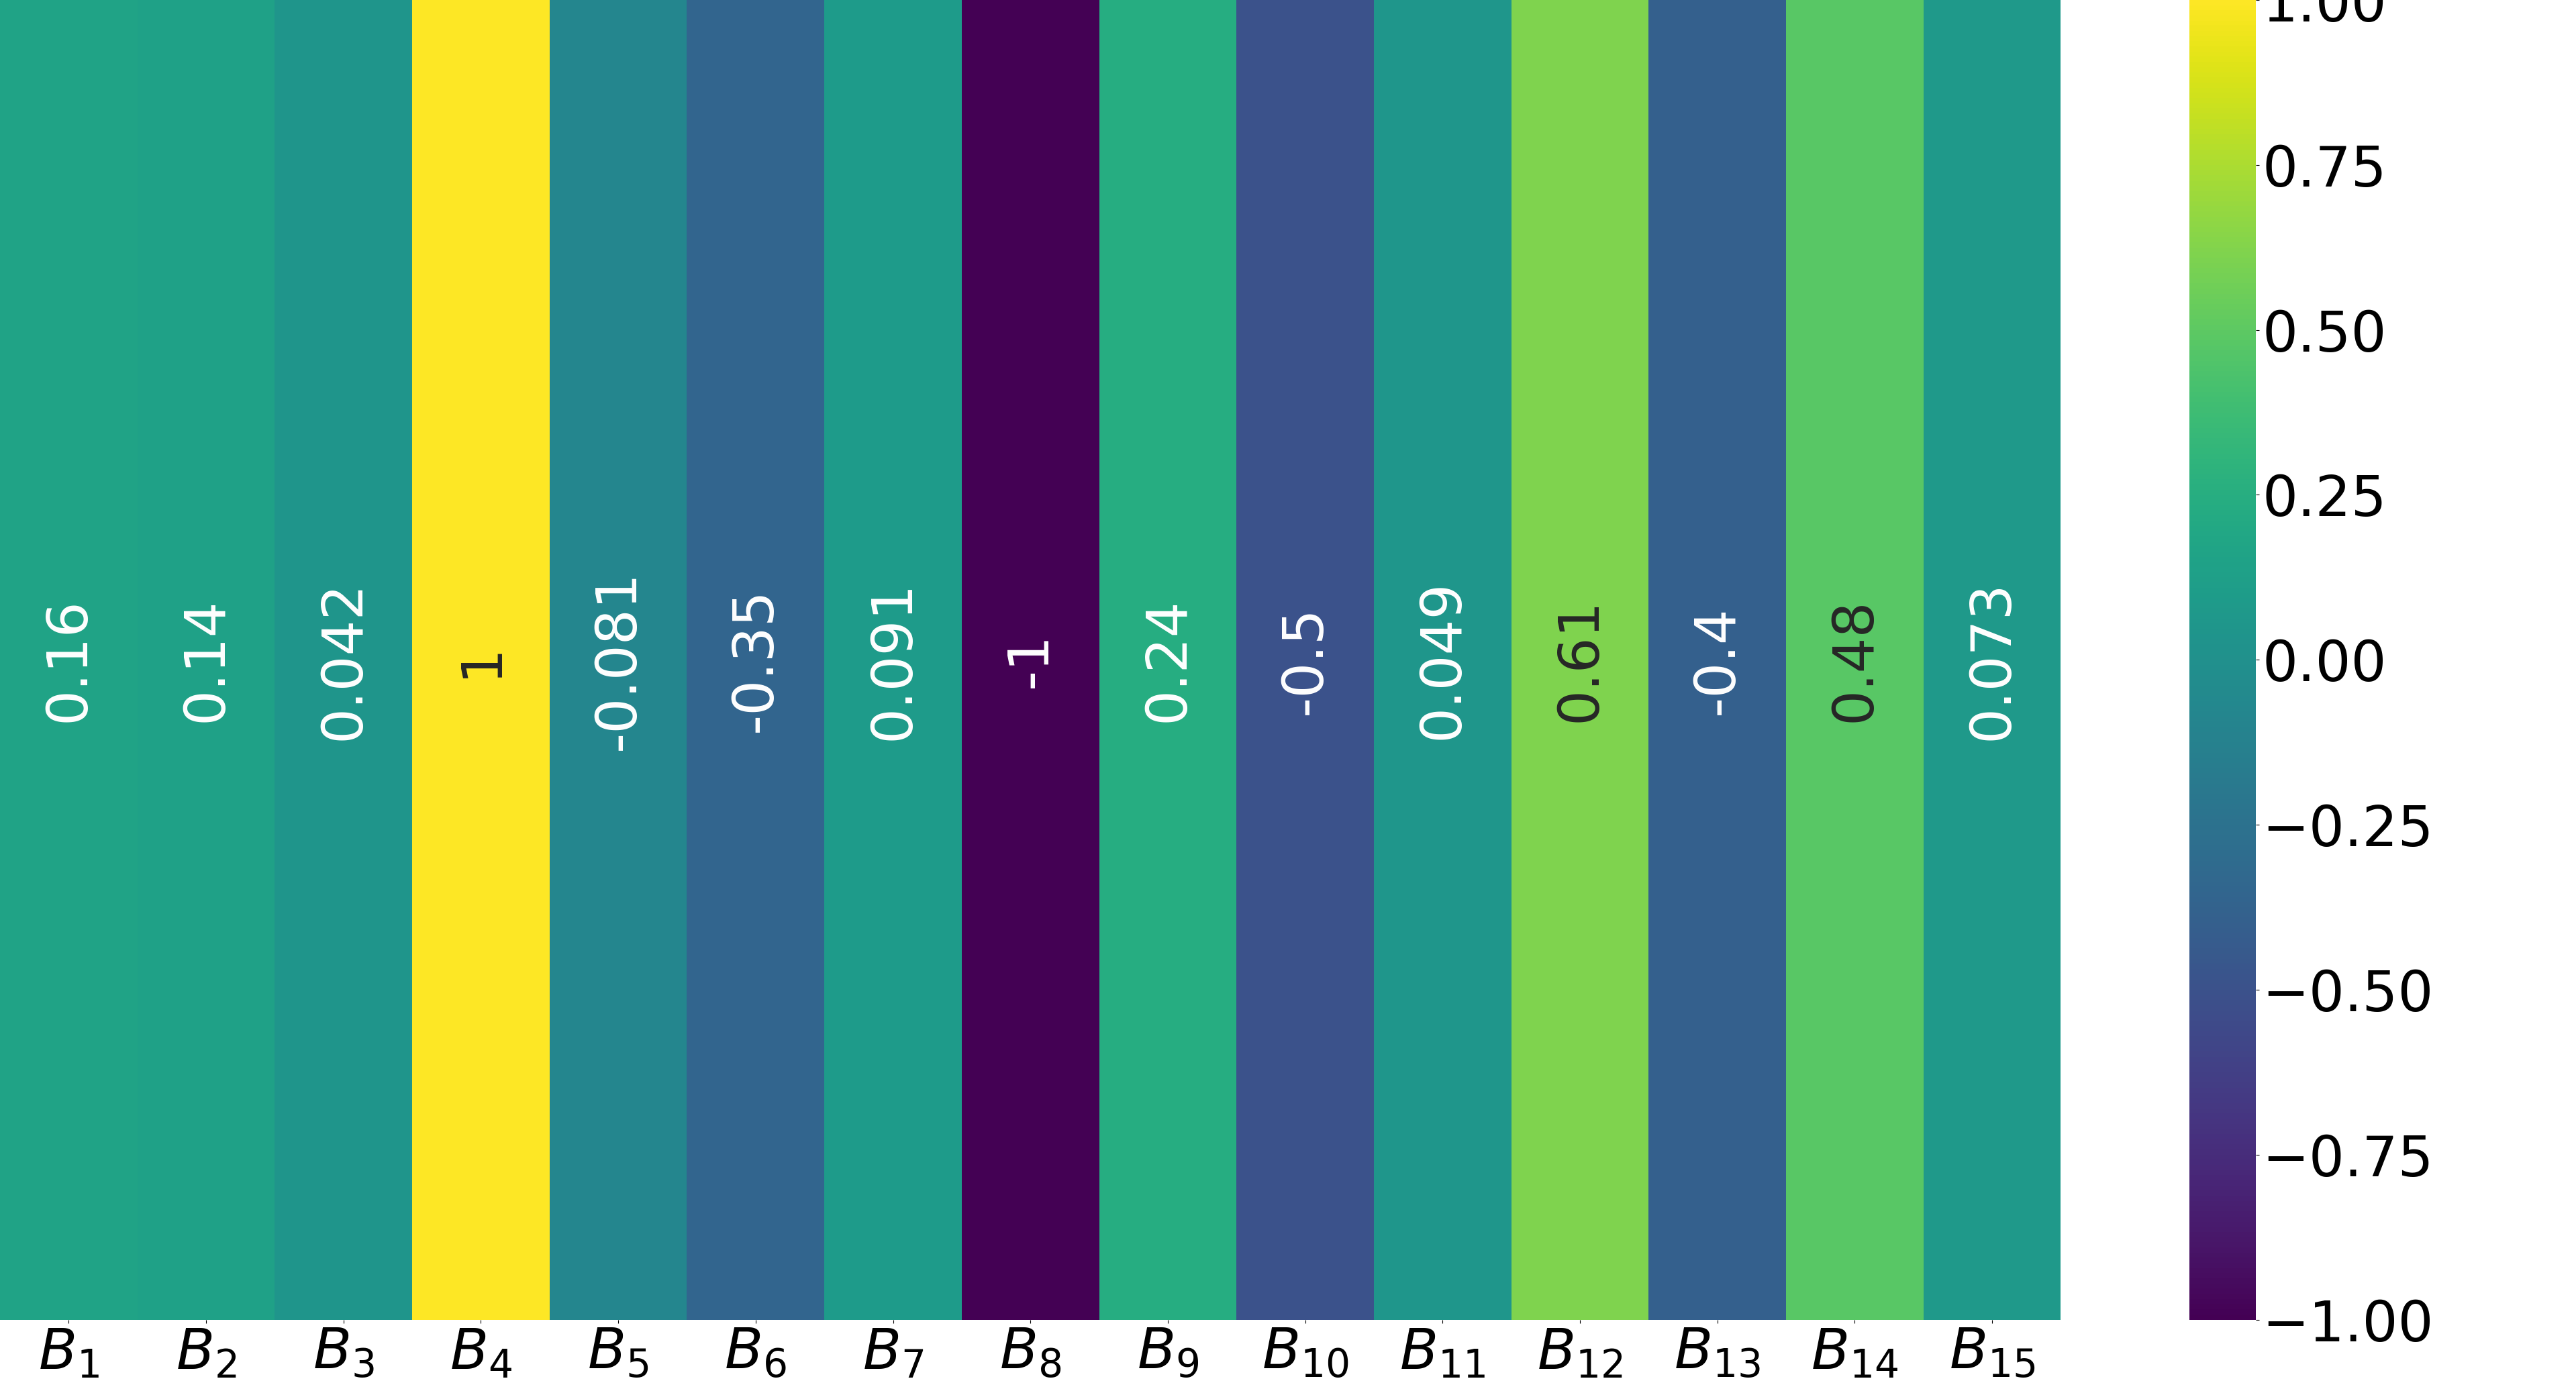
\includegraphics[width=\linewidth]{img/qlp_corr/Bn_coil2.png}
		\subcaption{Correlation with coil $2$}
	\end{subfigure}
	\begin{subfigure}{0.49\linewidth}
		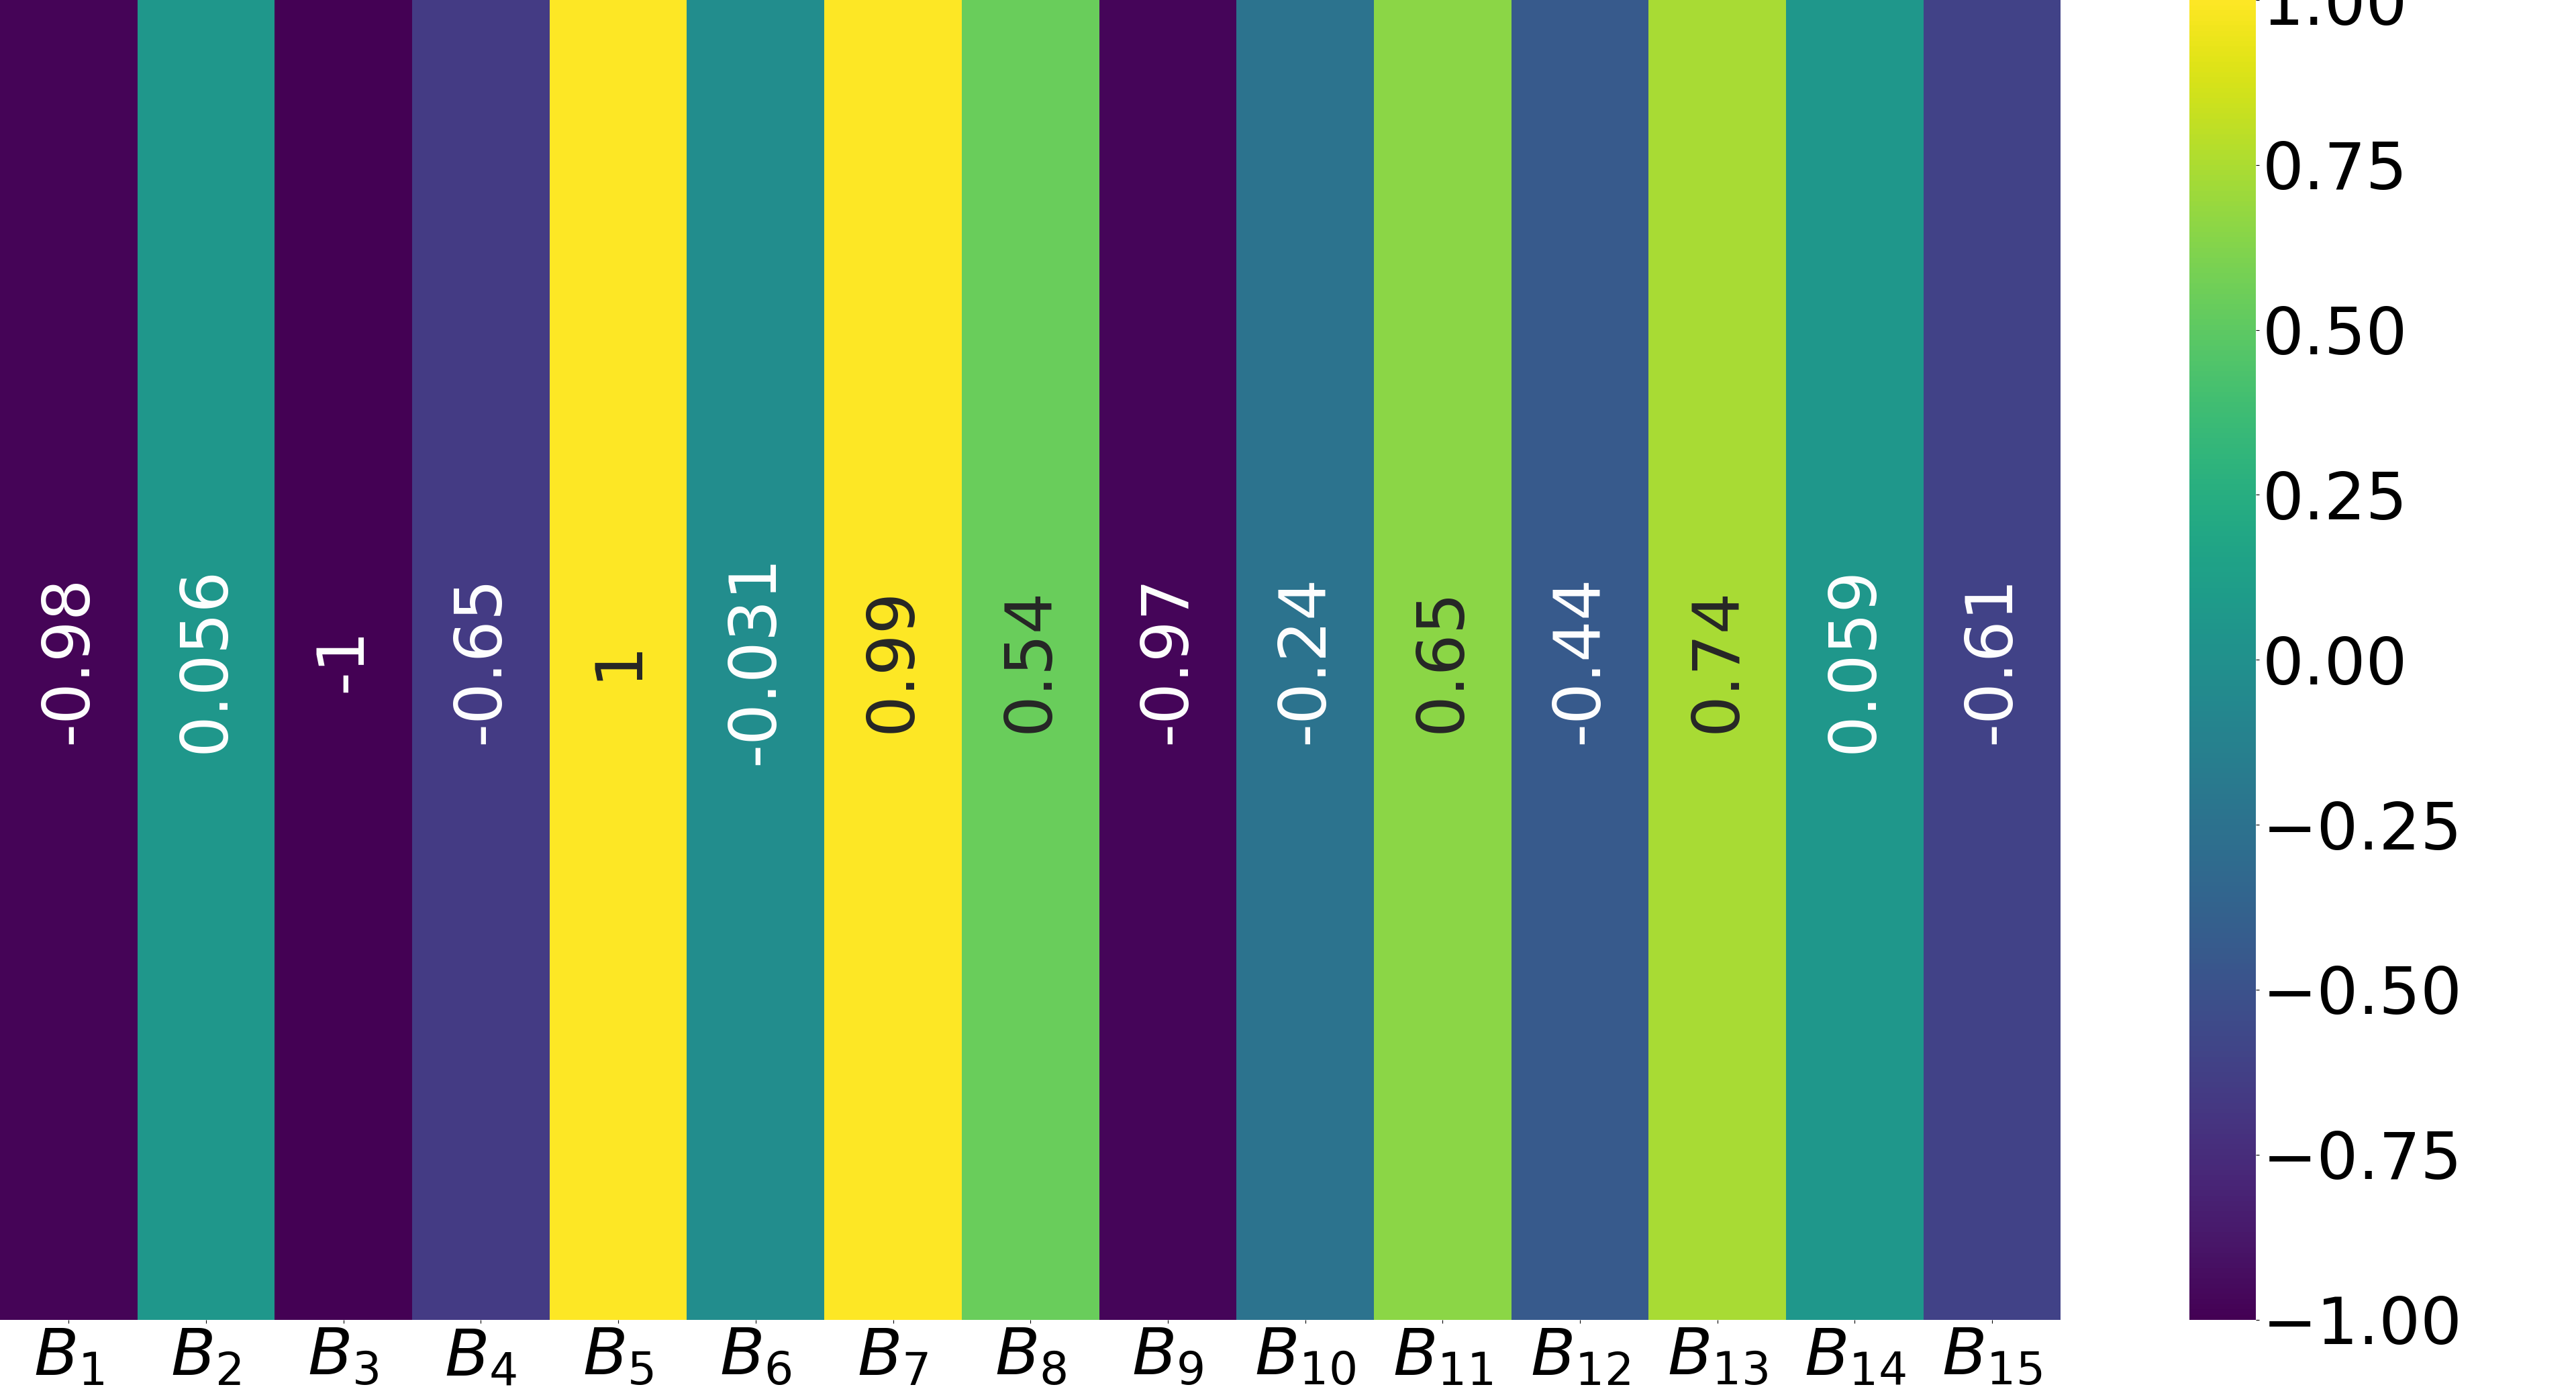
\includegraphics[width=\linewidth]{img/qlp_corr/Bn_coil3.png}
		\subcaption{Correlation with coil $3$}
	\end{subfigure}
	\caption{Correlation between the harmonics of the \bn\ attribute and the labels for \qlp.}
	\label{fig:bn-lcorr-qlp}
\end{figure}

In \Cref{fig:bn-coilq-dist} we visualized the samples in \bn\ after a round of \pca. Independently of the sub-figure we consider it's clear that the level of
homogeneity of the samples belonging to the central cluster is very high. While this, alone, cannot
induce us to think that the performance of models based on \bn\ is going to be bad, we are drawn to
consider the possibility that \bn\ might not be a good enough attribute if taken on its own.
\begin{figure}[!ht]
	% Font size = 40
	\centering
	\begin{subfigure}{0.8\linewidth}
		\centering
		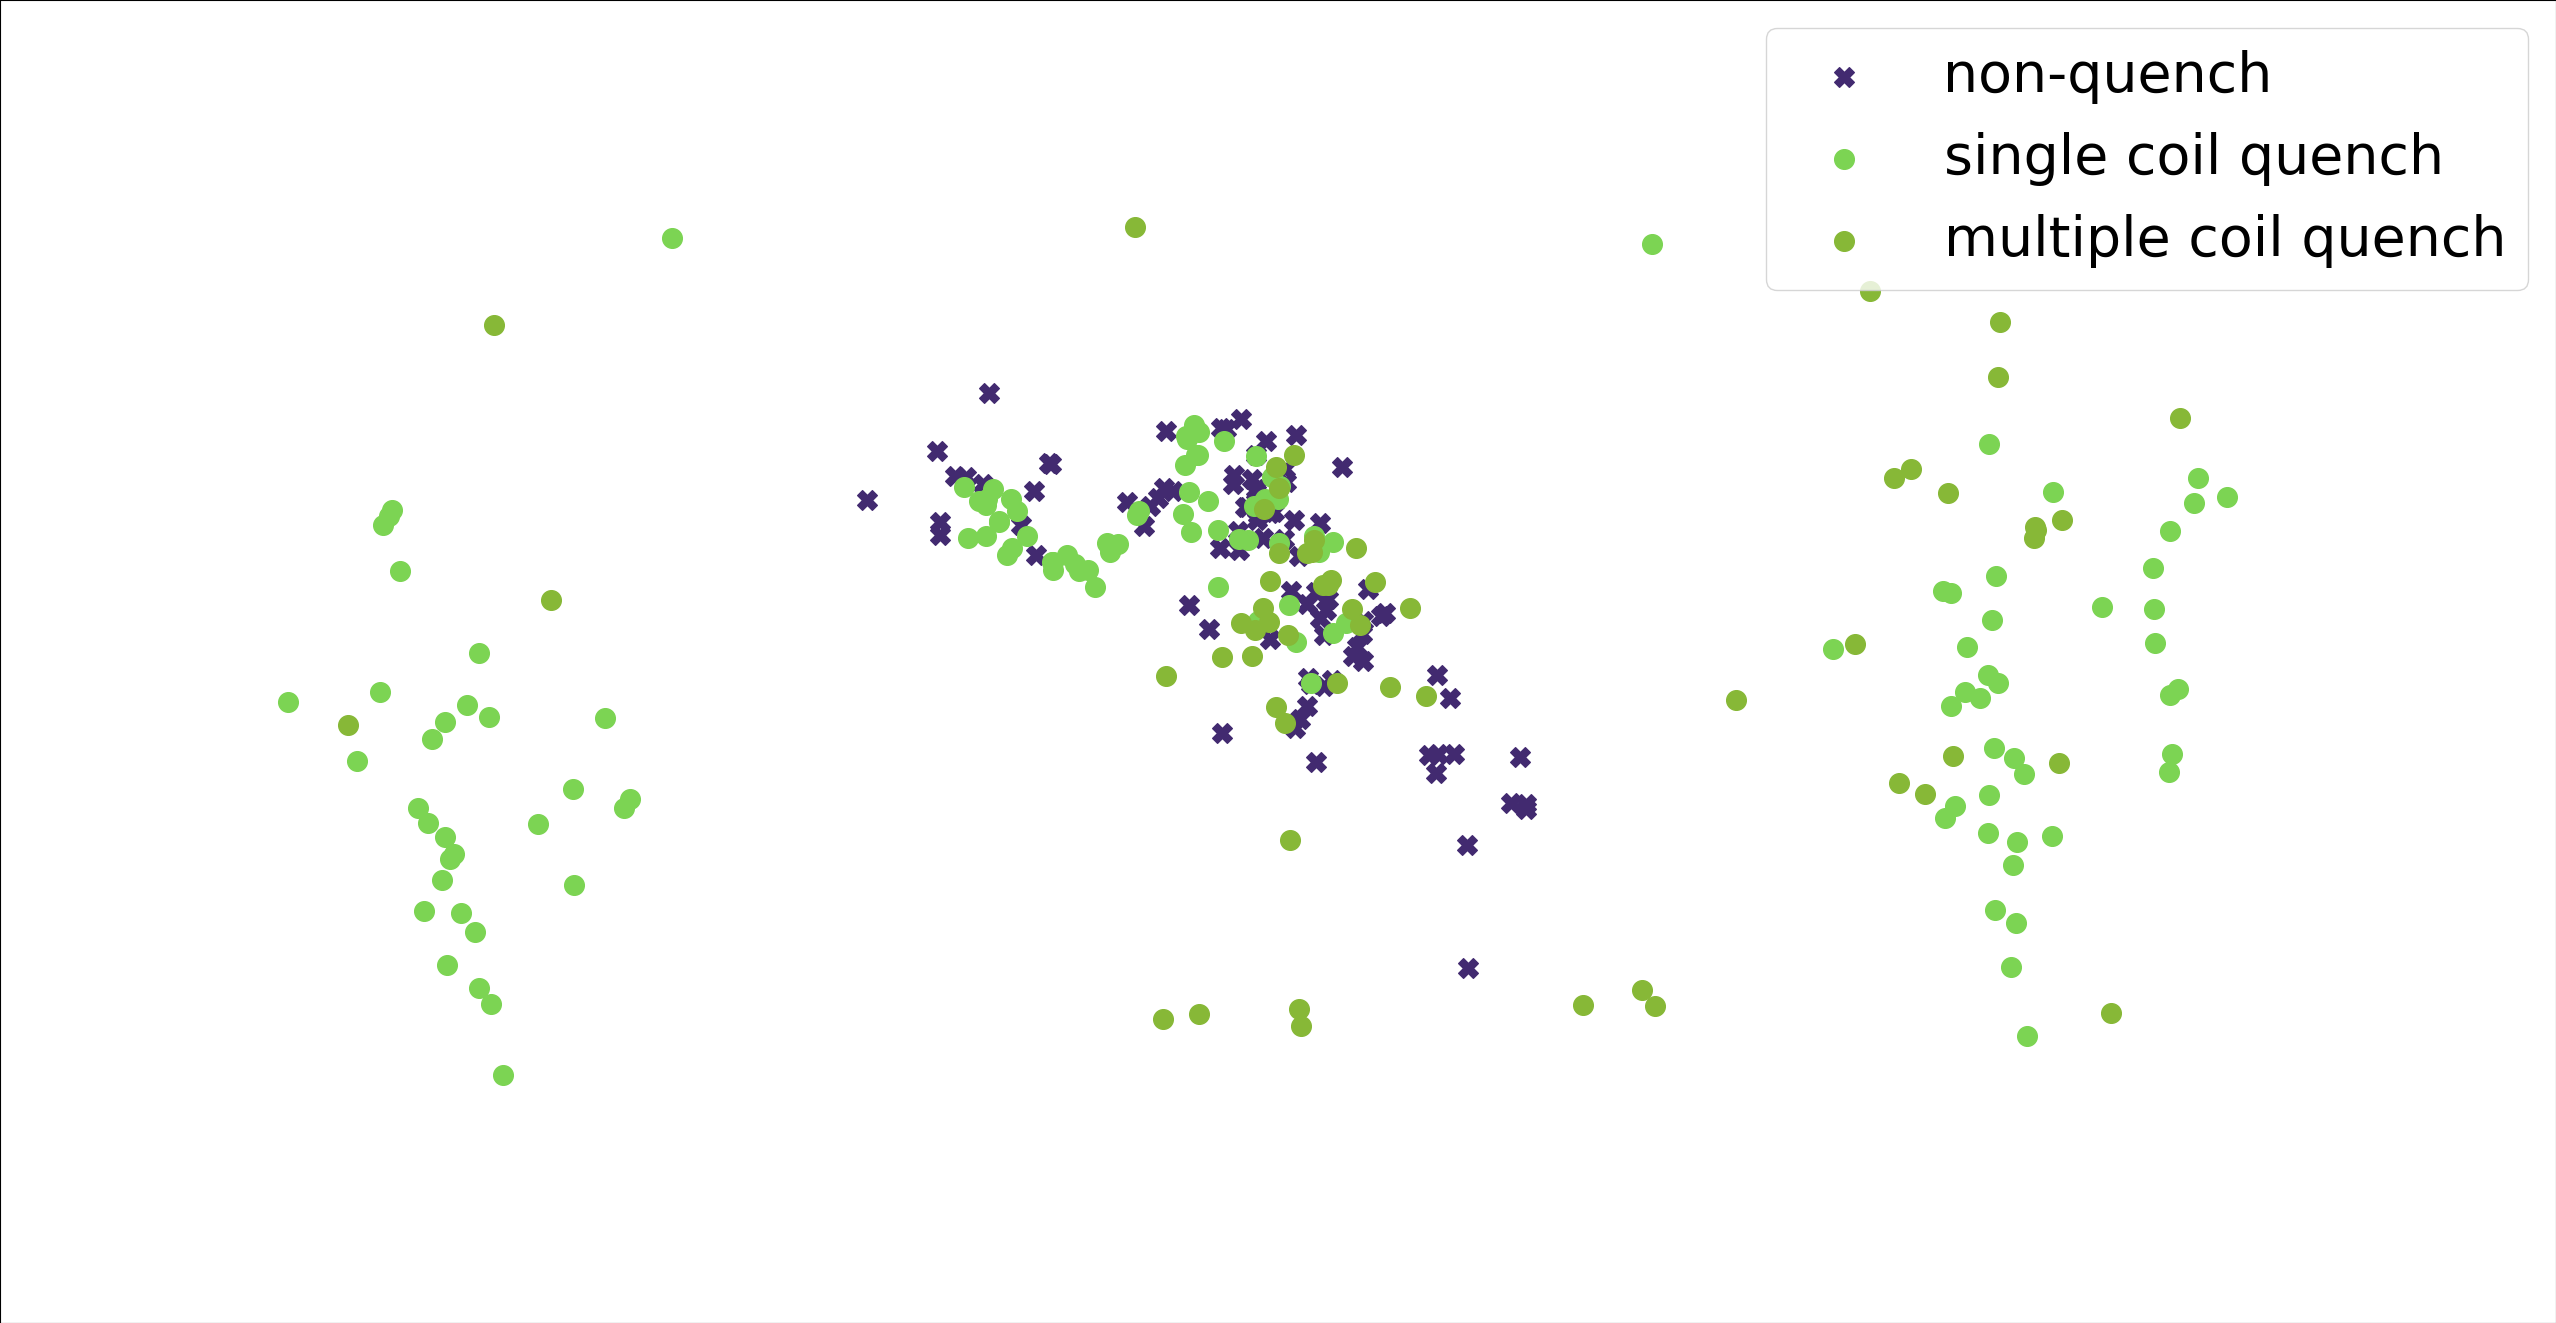
\includegraphics[width=\linewidth]{img/quench_dist_qlp/single_vs_multiple_Bn.png}
		\subcaption{}
	\end{subfigure}
	\begin{subfigure}{0.8\linewidth}
		\centering
		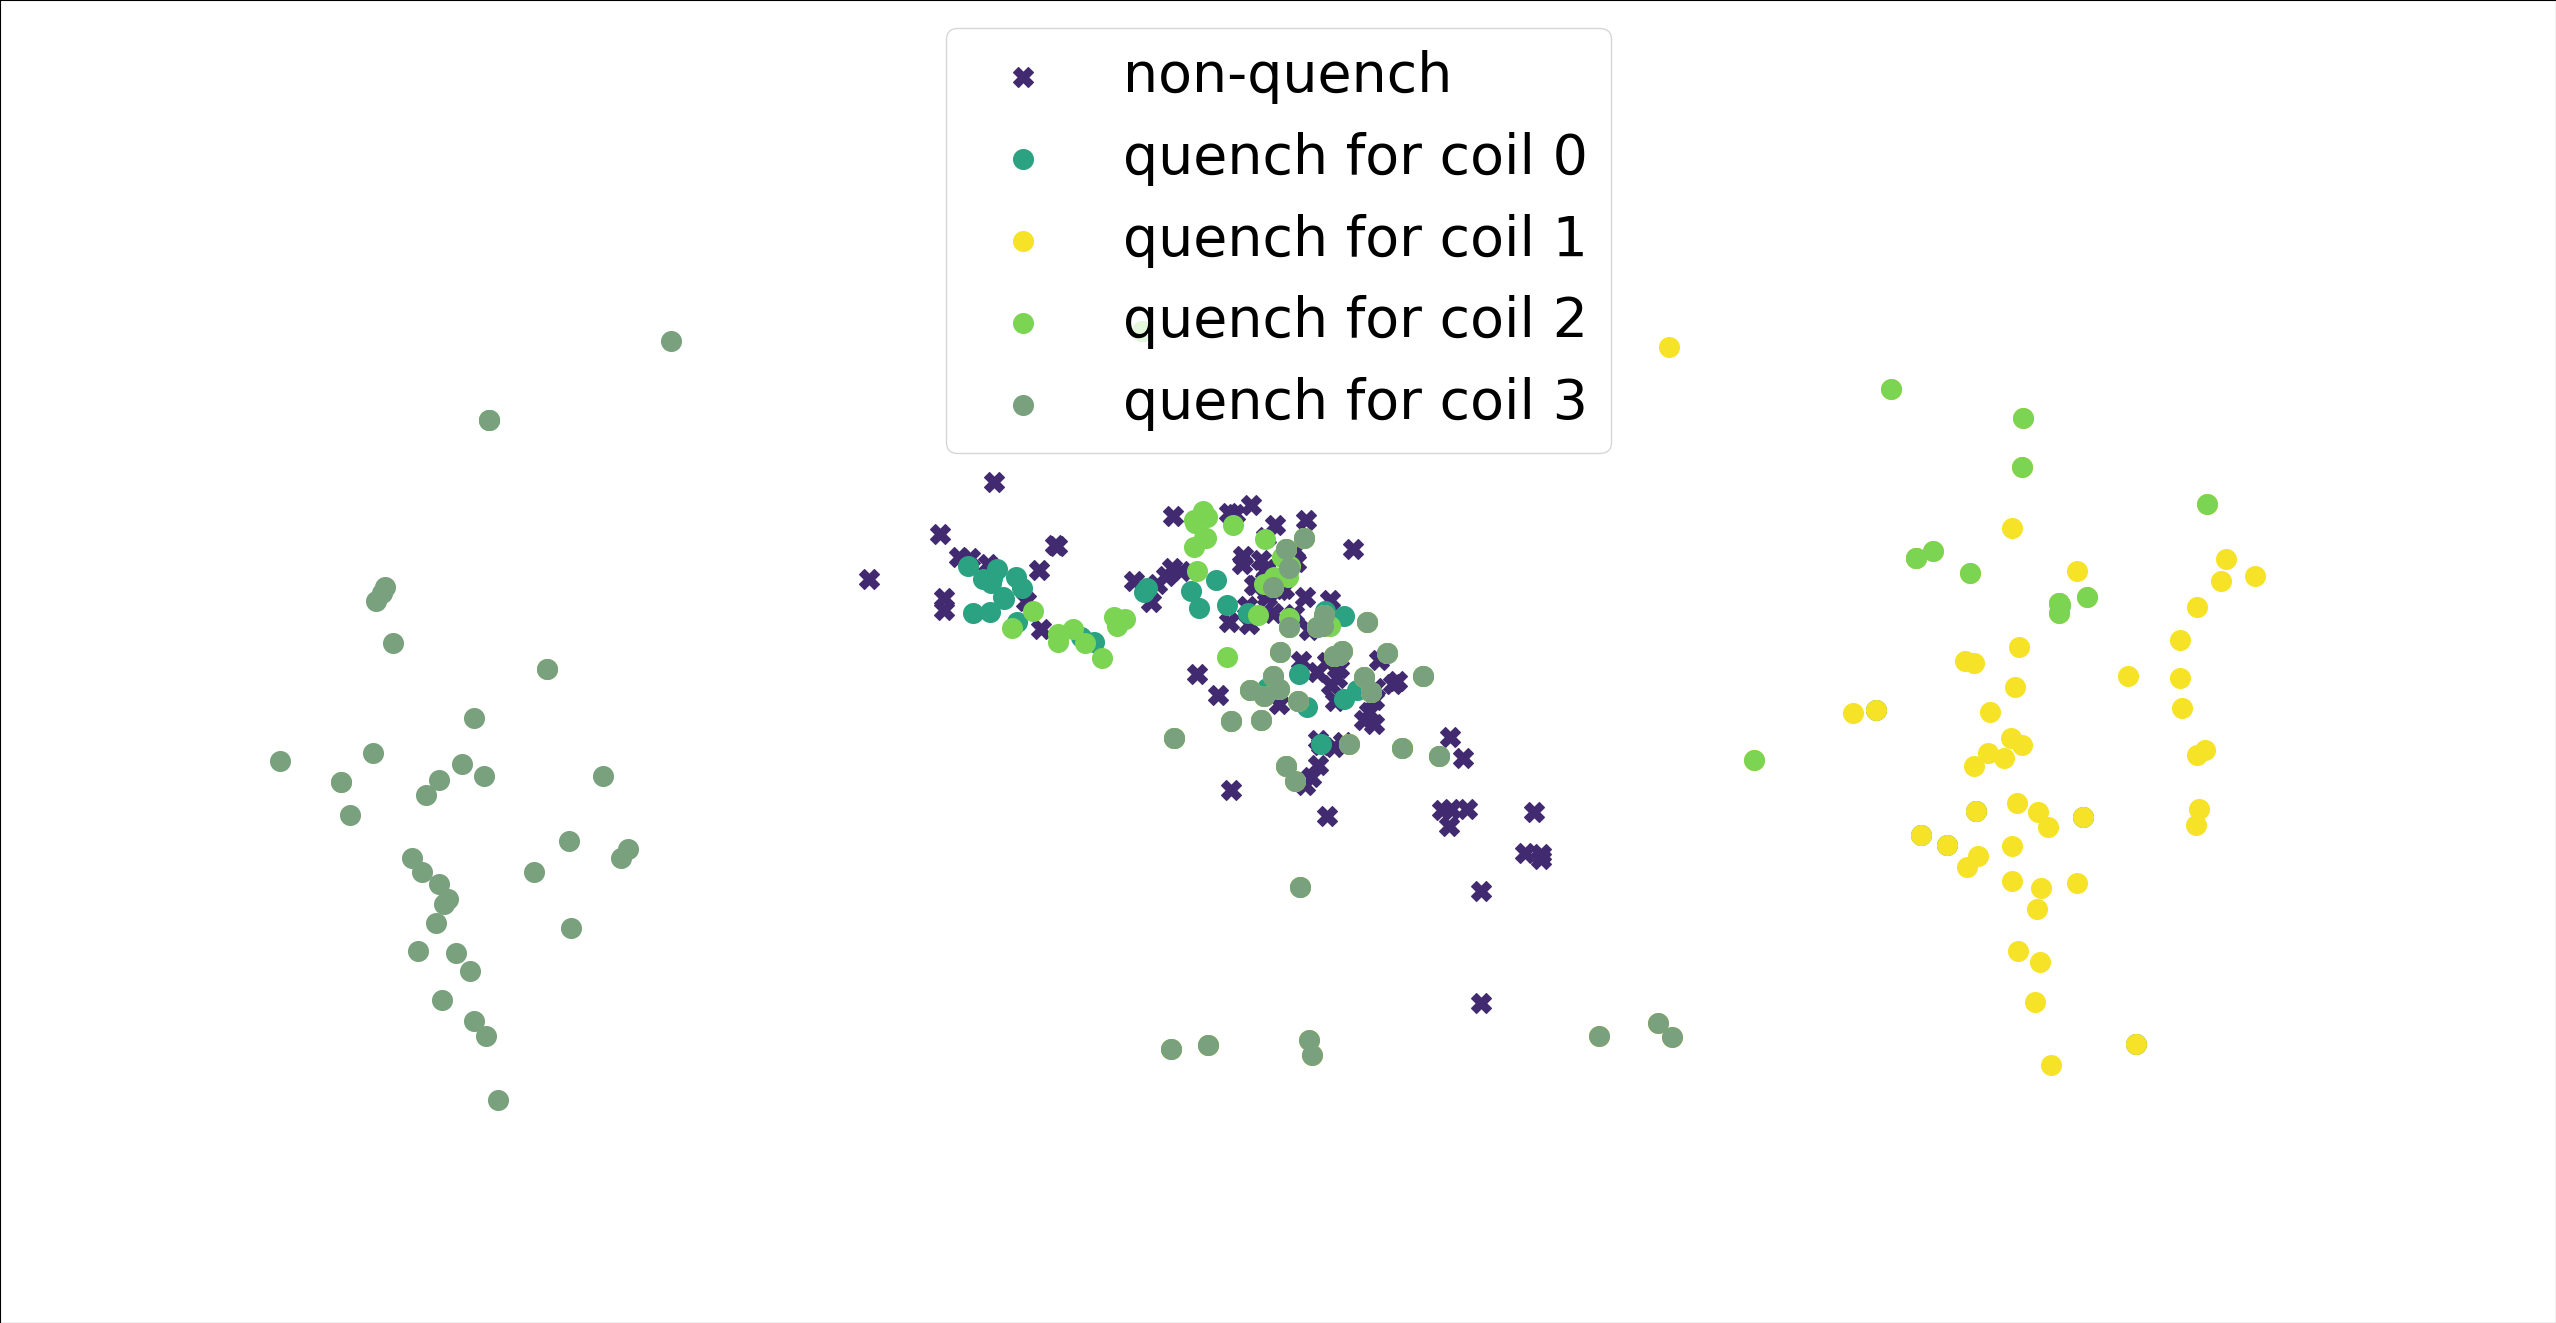
\includegraphics[width=\linewidth]{img/quench_dist_qlp_bn.png}
		\subcaption{}
	\end{subfigure}
	\caption{Visualization of the \bn\ attribute, the data was plotted after a run of \pca\
		dimensionality reduction. Sub-figure (a) highlights the samples based on how many quenches
		are associated to the specific sample $\{0, 1, \text{many}\}$. Sub-figure (b) highlights the
		samples based on the specific coil quenched $\{\text{None}, 0, 1, 2, 3\}$.}
	\label{fig:bn-coilq-dist}
\end{figure}

\subsubsection{\cnmod}
As we said in \Cref{chp:problem}, \cnmod\ was expected to be very informative for \qrp, but not for
\qlp. Interestingly, though, the correlation between the harmonics for the attribute and the labels
associated to each coil, shown in \Cref{fig:cnmod-lcorr-qlp}, seem to be telling a different story.
If we consider coils $0$ and $3$, we can see a very strong correlation between the harmonics and the
label, it's also worth noting that, in sub-figures (a) through (d), \cnmod[2]\ seems to be extremely
important to explain the value associated with the labels.

If we look back at the correlation matrix computed for \cnmod\ during the preprocessing for \qrp\
(cfr. \Cref{fig:cnmod-corr}) a sub-view of \cnmod\ could be built as follows:
\begin{itemize}
	\item For coil $0$, \cnmod[2] and adding a high-order candidate. While this would technically maximize the total correlation with the label, we have seen in \qrp\ that choosing \cnmod[2]\ was a choice that didn't pay. That is why we might select \cnmod[3] or \cnmod[6] in the end, accompanied by another high order harmonic like \cnmod[9] or \cnmod[11].
	\item For coil $3$, we could be taking harmonic \cnmod[1] and then using one or more from
	      \{\cnmod[4], \cnmod[5], \cnmod[6], \cnmod[7], \cnmod[8]\}; finally, if it leads to
	      better performance, we could also add another high-order harmonic like \cnmod[10].
\end{itemize}
\begin{figure}[!ht]
	% Font size = 70
	\centering
	\begin{subfigure}{0.49\linewidth}
		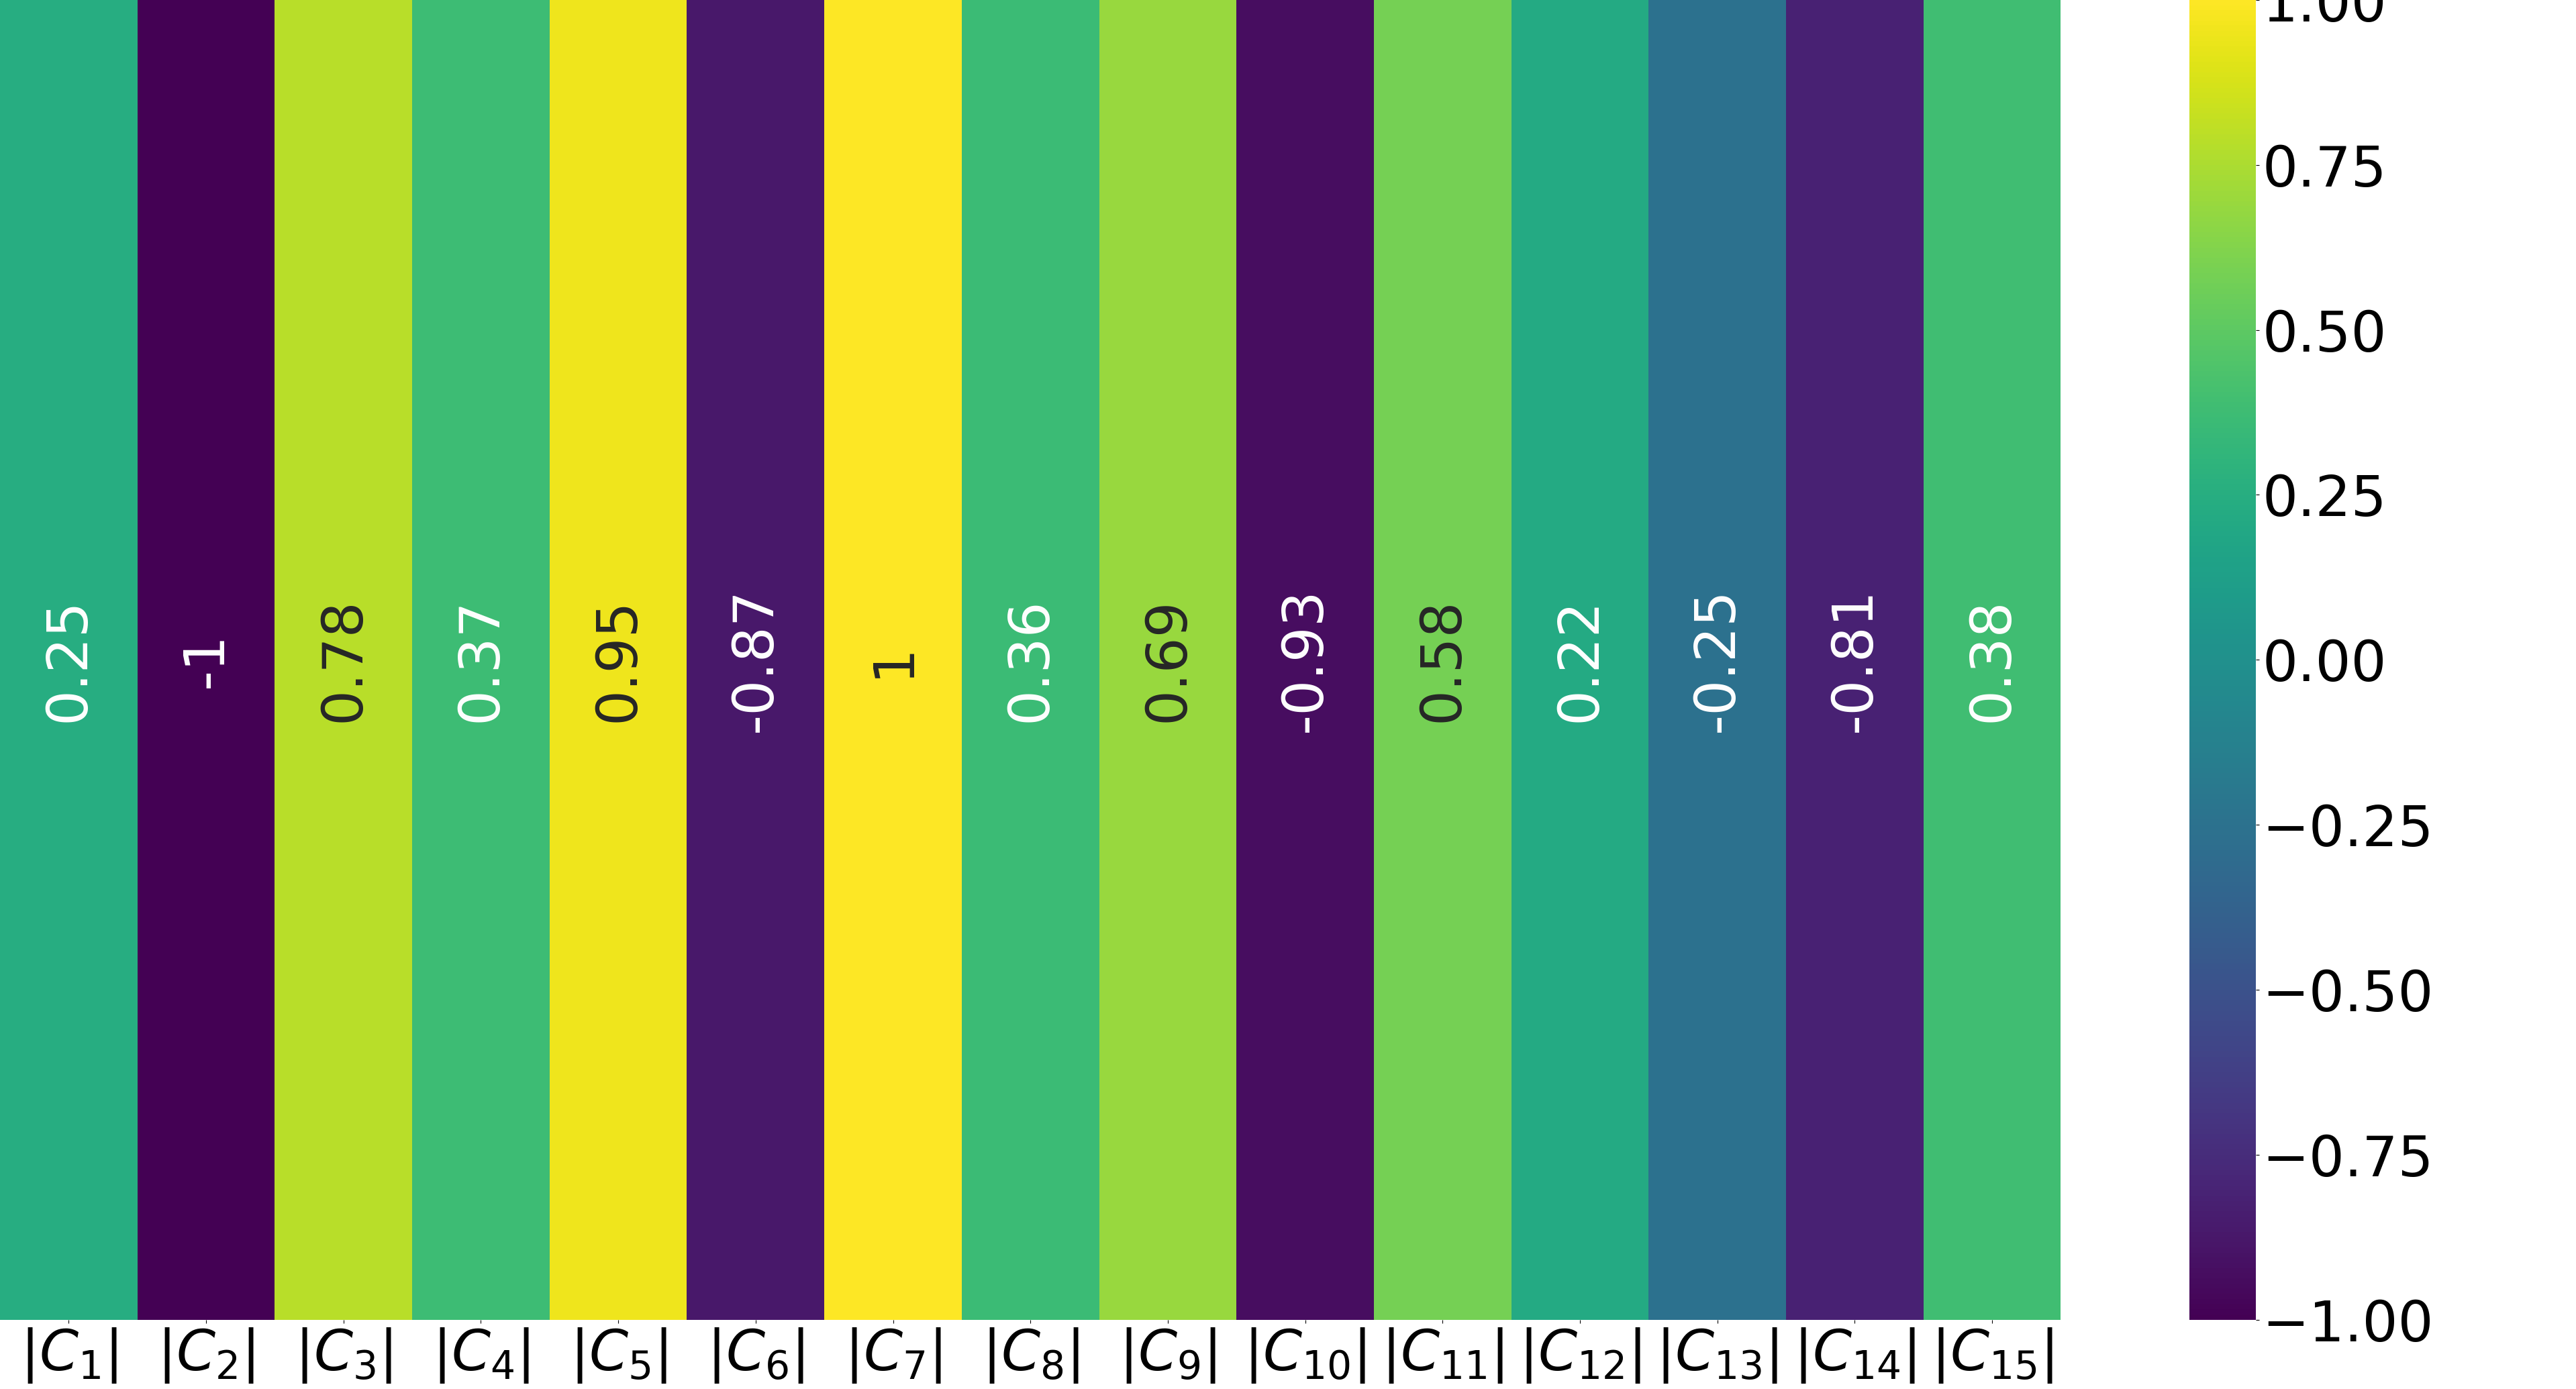
\includegraphics[width=\linewidth]{img/qlp_corr/Cnmod_coil0.png}
		\subcaption{Correlation with coil $0$}
	\end{subfigure}
	\begin{subfigure}{0.49\linewidth}
		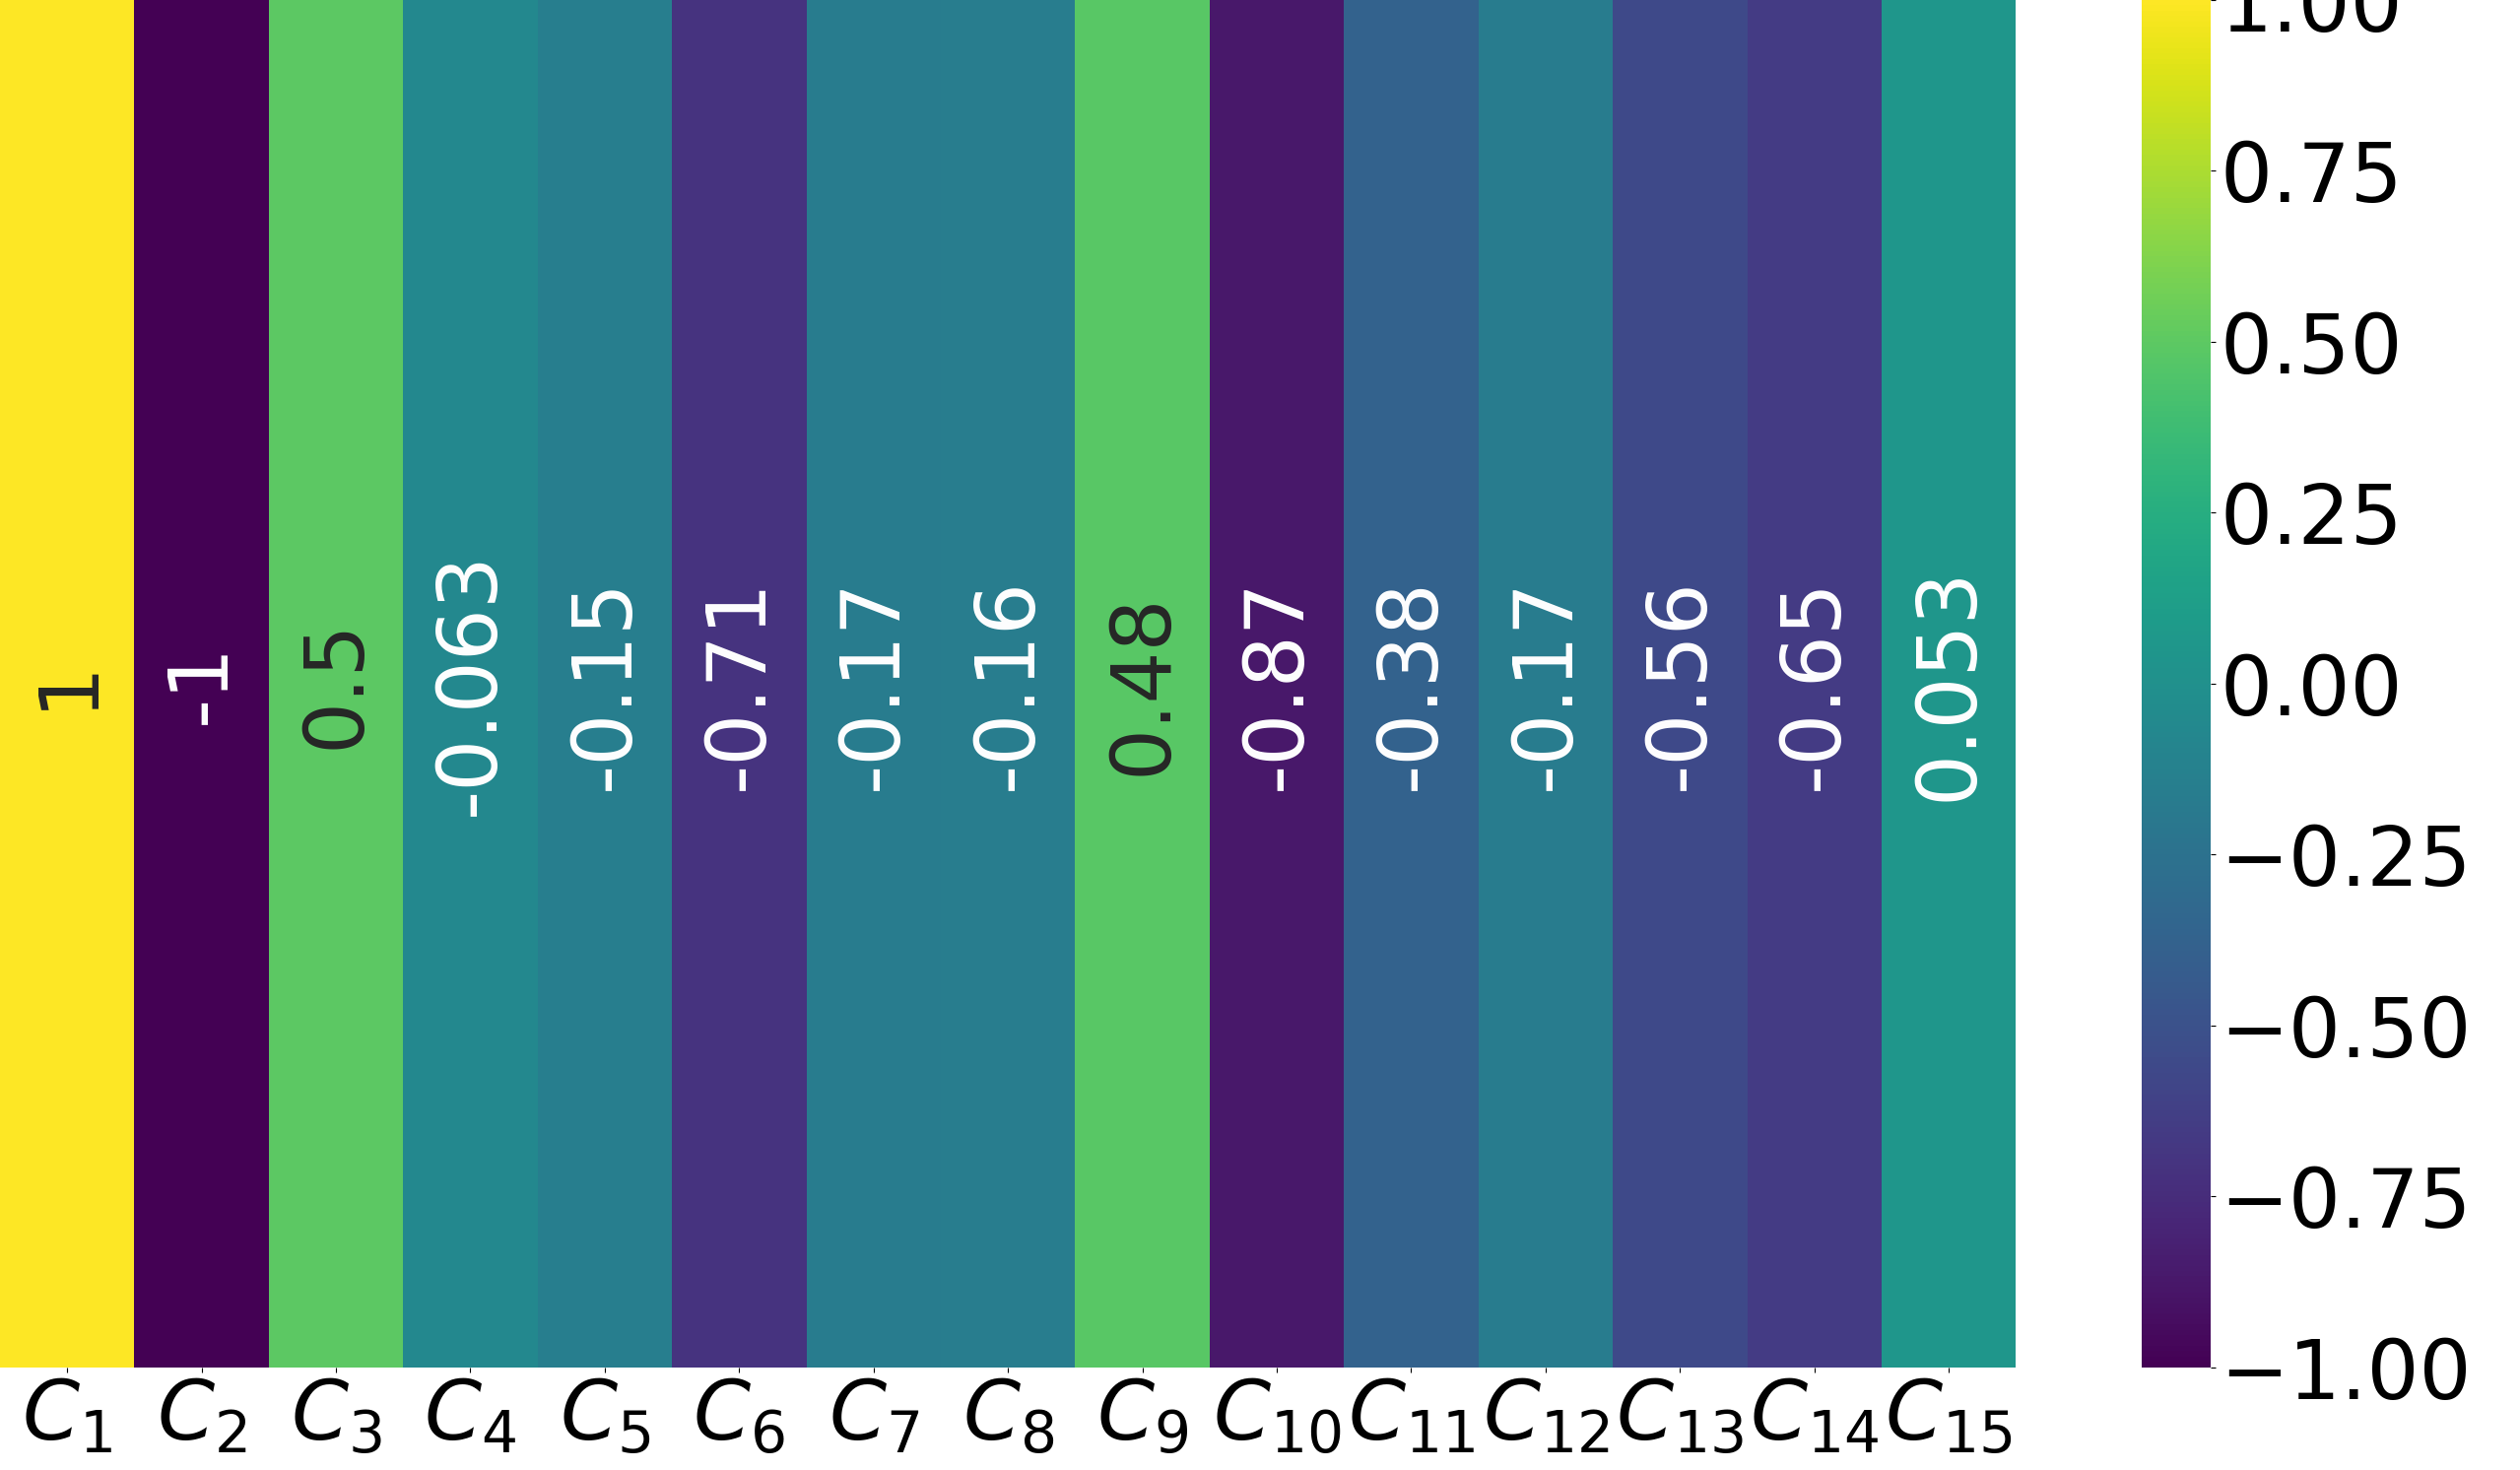
\includegraphics[width=\linewidth]{img/qlp_corr/Cnmod_coil1.png}
		\subcaption{Correlation with coil $1$}
	\end{subfigure}
	\begin{subfigure}{0.49\linewidth}
		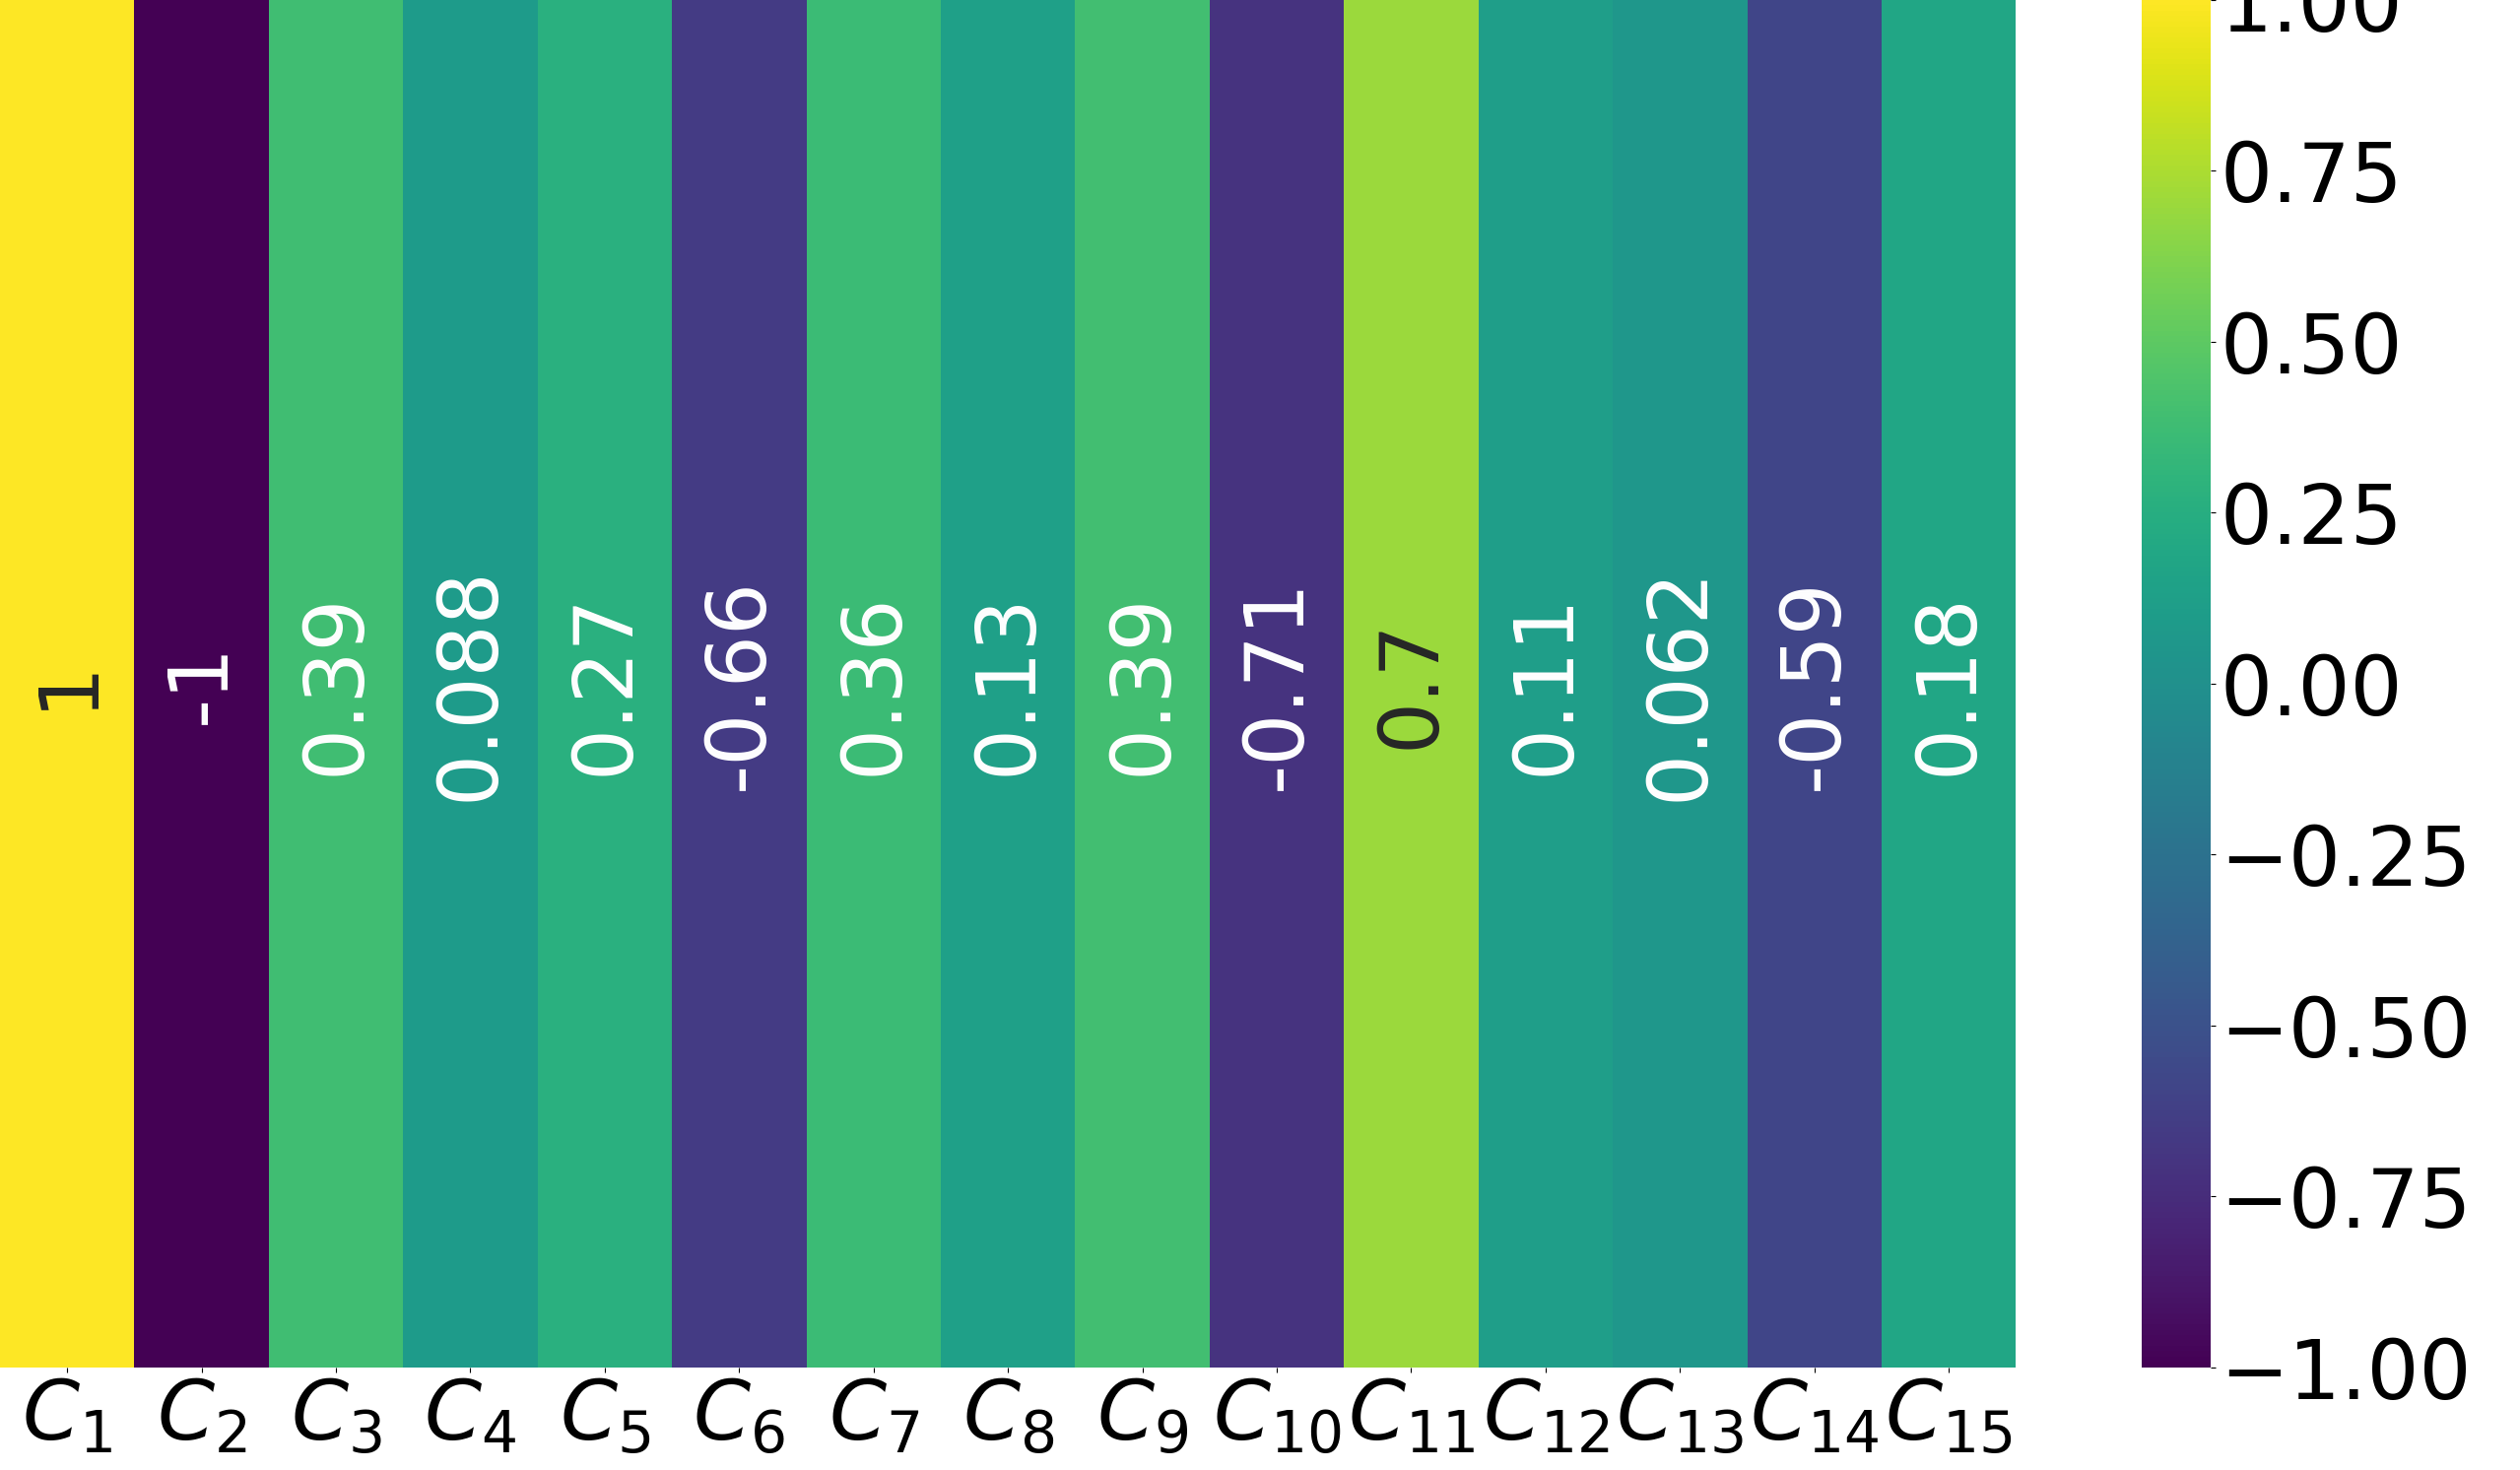
\includegraphics[width=\linewidth]{img/qlp_corr/Cnmod_coil2.png}
		\subcaption{Correlation with coil $2$}
	\end{subfigure}
	\begin{subfigure}{0.49\linewidth}
		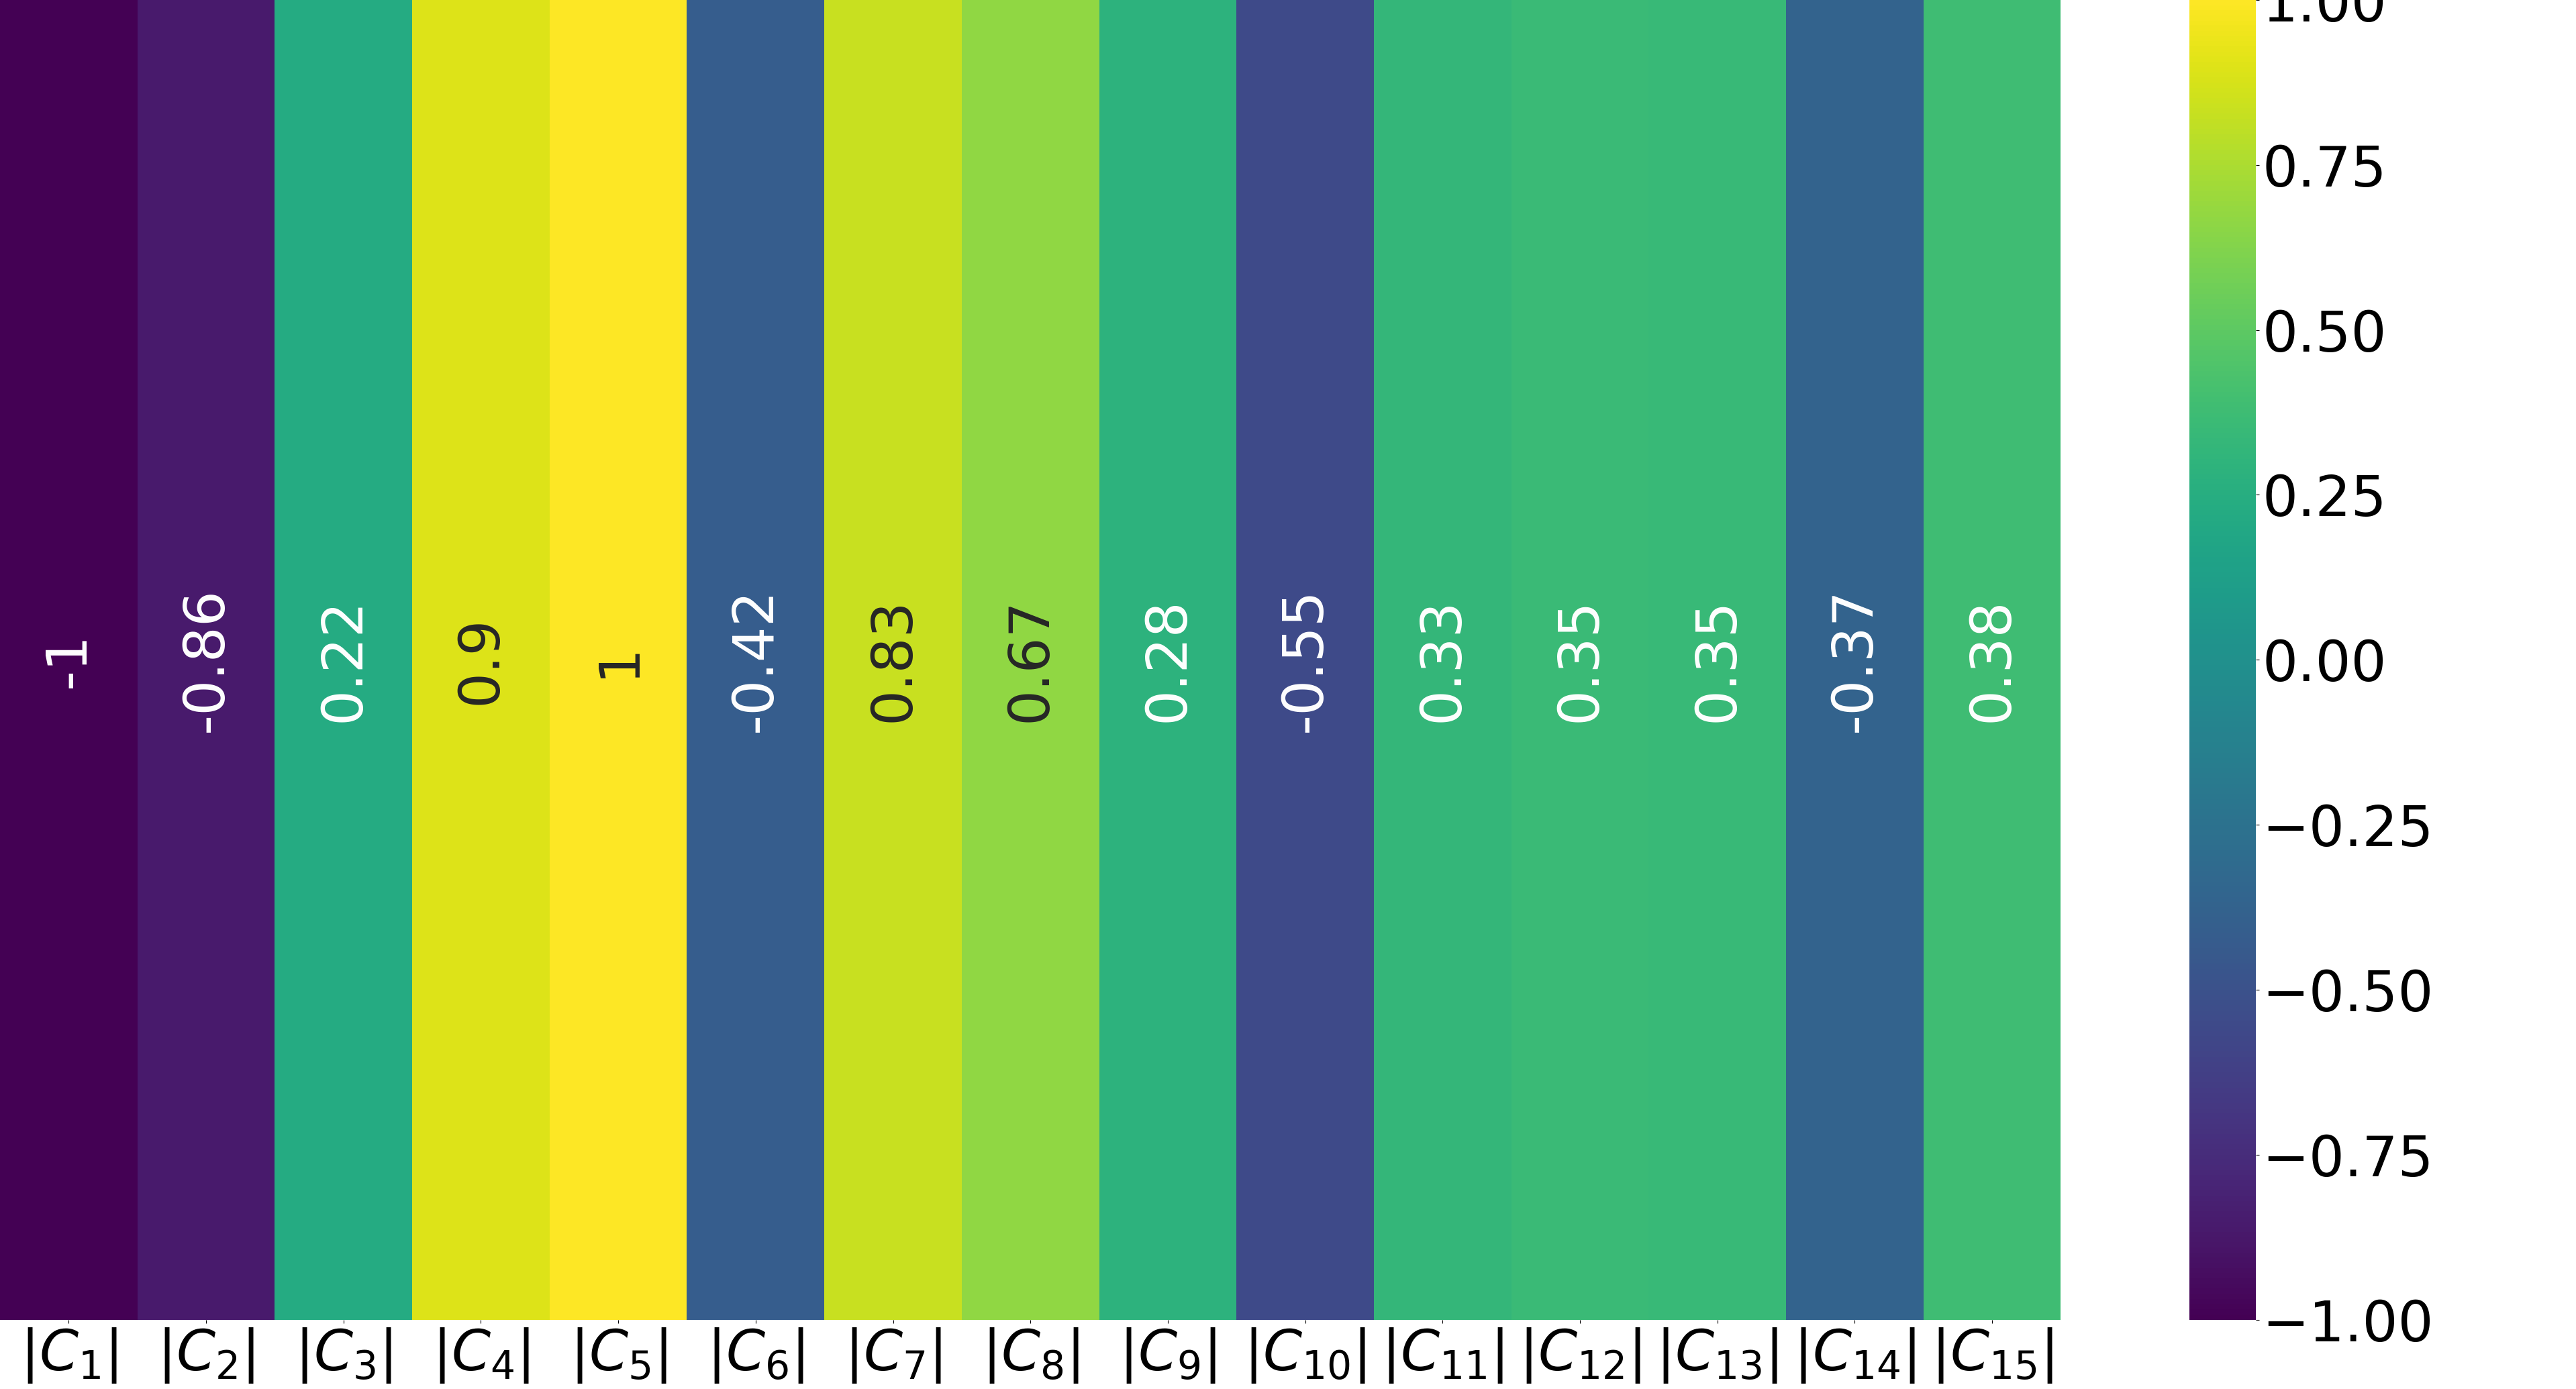
\includegraphics[width=\linewidth]{img/qlp_corr/Cnmod_coil3.png}
		\subcaption{Correlation with coil $3$}
	\end{subfigure}
	\caption{Correlation between the harmonics of the \cnmod\ attribute and the labels for \qlp.}
	\label{fig:cnmod-lcorr-qlp}
\end{figure}

As we did for \an\ and \bn, we visualized \cnmod\ after a round of \pca\ dimensionality reduction.
\Cref{fig:cnmod-coilq-dist} shows a similar situation to \an, if we consider the specific case of
sub-figure (a), while the clusters are not as clean cut as the alternative, there is much more
separation of the classes compared to \bn. As far as single coil quench is concerned (cfr. sub-figure
(b)), there is clearly a high degree of homogeneity due to having many groups of points labelled
differently but extremely close together.
\begin{figure}[!ht]
	% Font size = 40
	\centering
	\begin{subfigure}{0.8\linewidth}
		\centering
		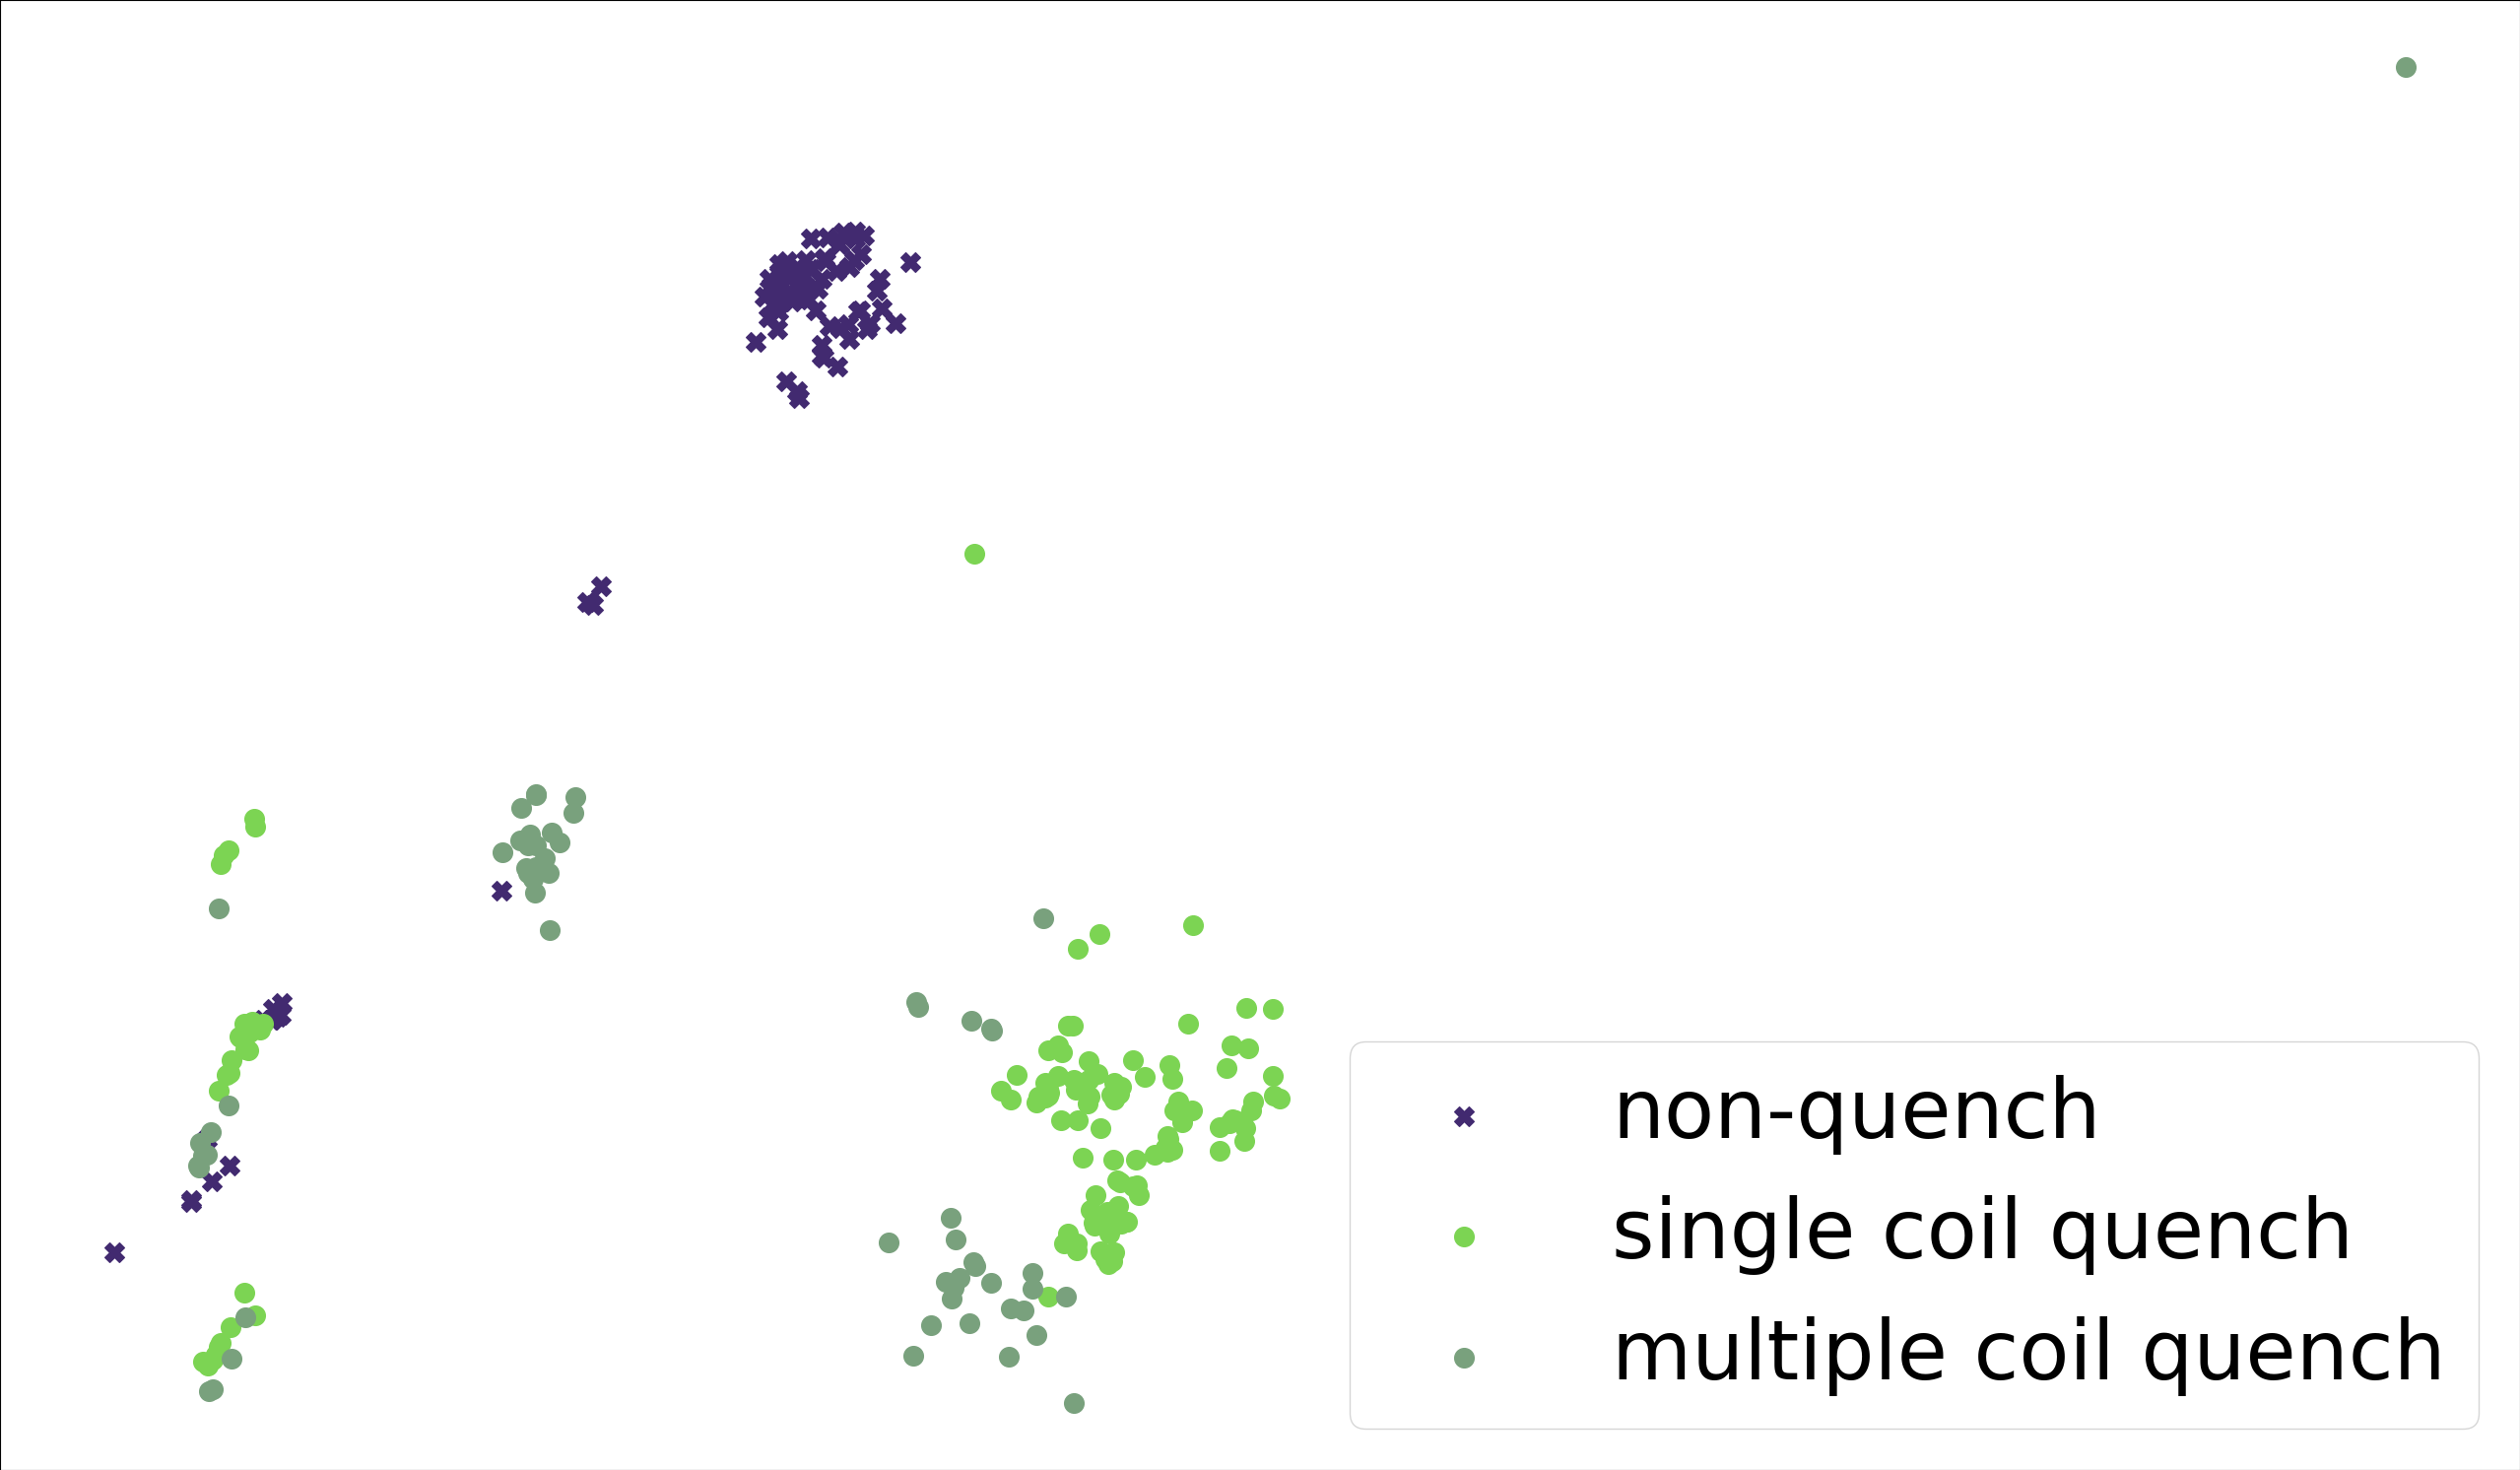
\includegraphics[width=\linewidth]{img/quench_dist_qlp/single_vs_multiple_Cnmod.png}
		\subcaption{}
	\end{subfigure}
	\begin{subfigure}{0.8\linewidth}
		\centering
		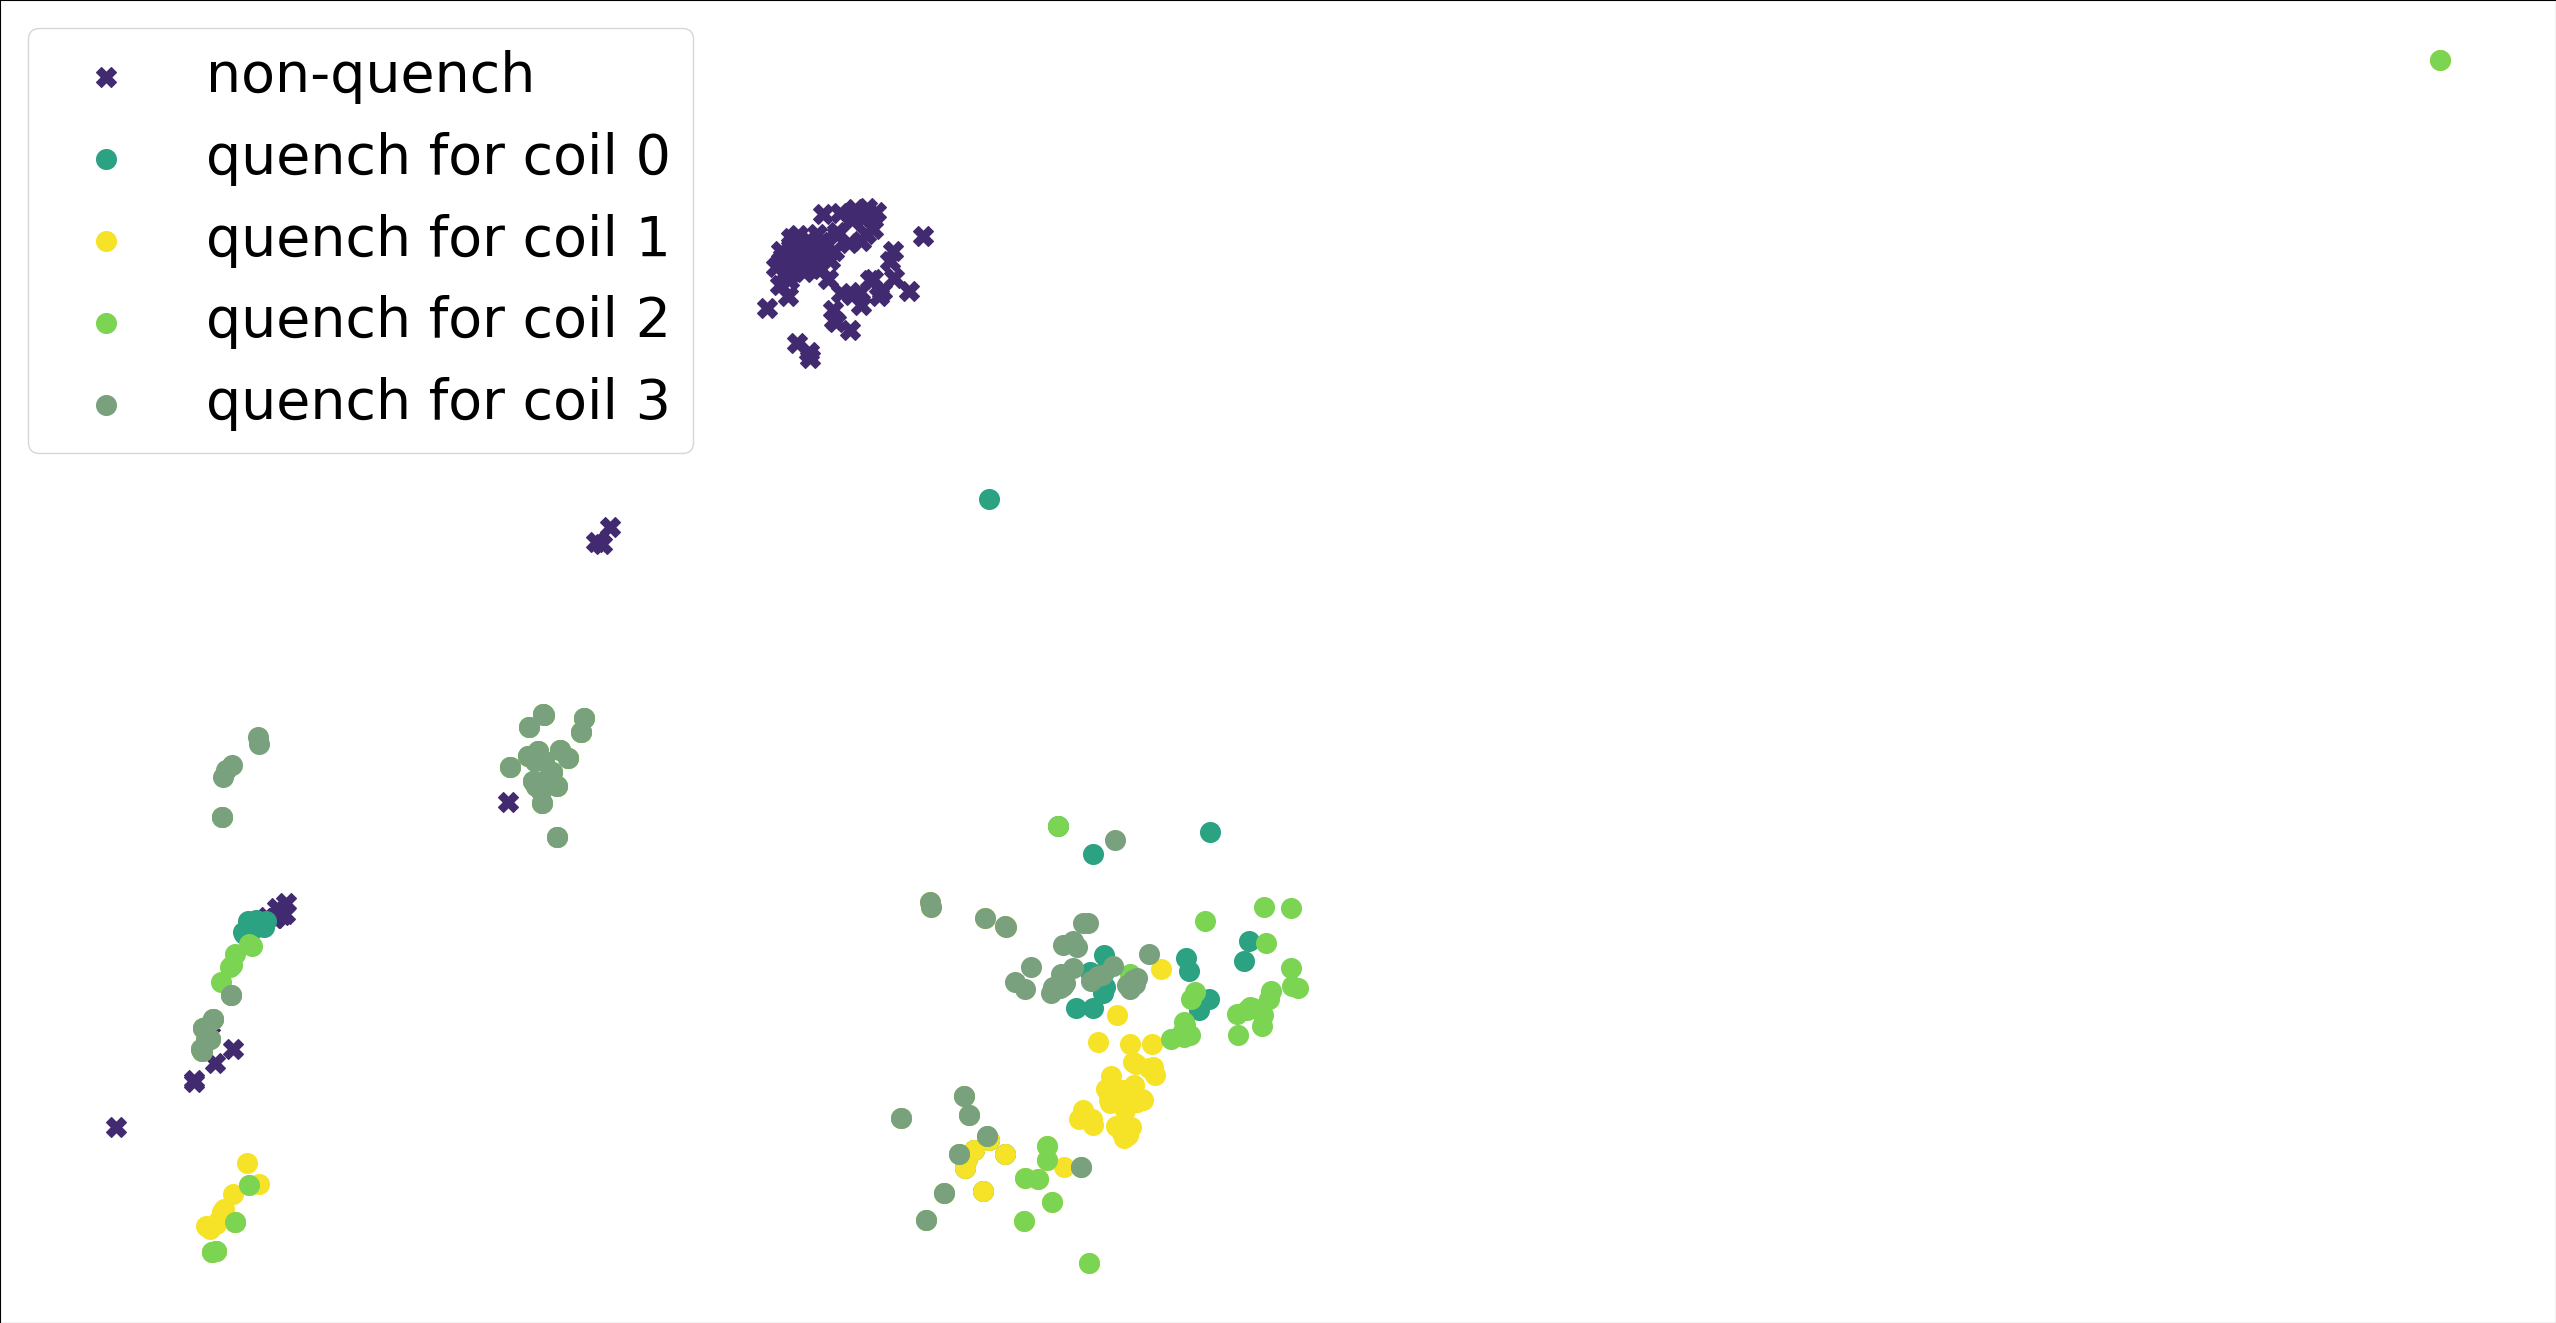
\includegraphics[width=\linewidth]{img/quench_dist_qlp_cnmod.png}
		\subcaption{}
	\end{subfigure}
	\caption{Visualization of the \cnmod\ attribute, the data was plotted after a run of \pca\
		dimensionality reduction. Sub-figure (a) highlights the samples based on how many quenches
		are associated to the specific sample $\{0, 1, \text{many}\}$. Sub-figure (b) highlights the
		samples based on the specific coil quenched $\{\text{None}, 0, 1, 2, 3\}$.}
	\label{fig:cnmod-coilq-dist}
\end{figure}

\subsubsection{\phin}
To close the section we are going to consider the \phin\ attribute. In \Cref{fig:phi-lcorr-qlp} we
plotted the cross-correlation between the harmonics and the labels. Due to how high the correlation
is between most harmonics and basically all the coils, we might be lead to think that this is the
best attribute available to us. Since the harmonics are also very weakly correlated among themselves
(cfr. \Cref{fig:phi-corr}), we just chose to not extract any features and keep the attribute as is.
On the other hand, the bidimensional visualization of the data is telling a different story (cfr.
\Cref{fig:phi-coilq-dist}), closer, as a matter of fact, to what we discovered for \bn.

\Cref{fig:phi-coilq-dist} plots the data after a round of \pca\ dimensionality reduction.
Independently of the sub-figure we consider, the sparsity and the homogeneity of the data makes it
extremely hard to define clusters with a high level of purity.
\begin{figure}[!ht]
	% Font size = 70
	\centering
	\begin{subfigure}{0.49\linewidth}
		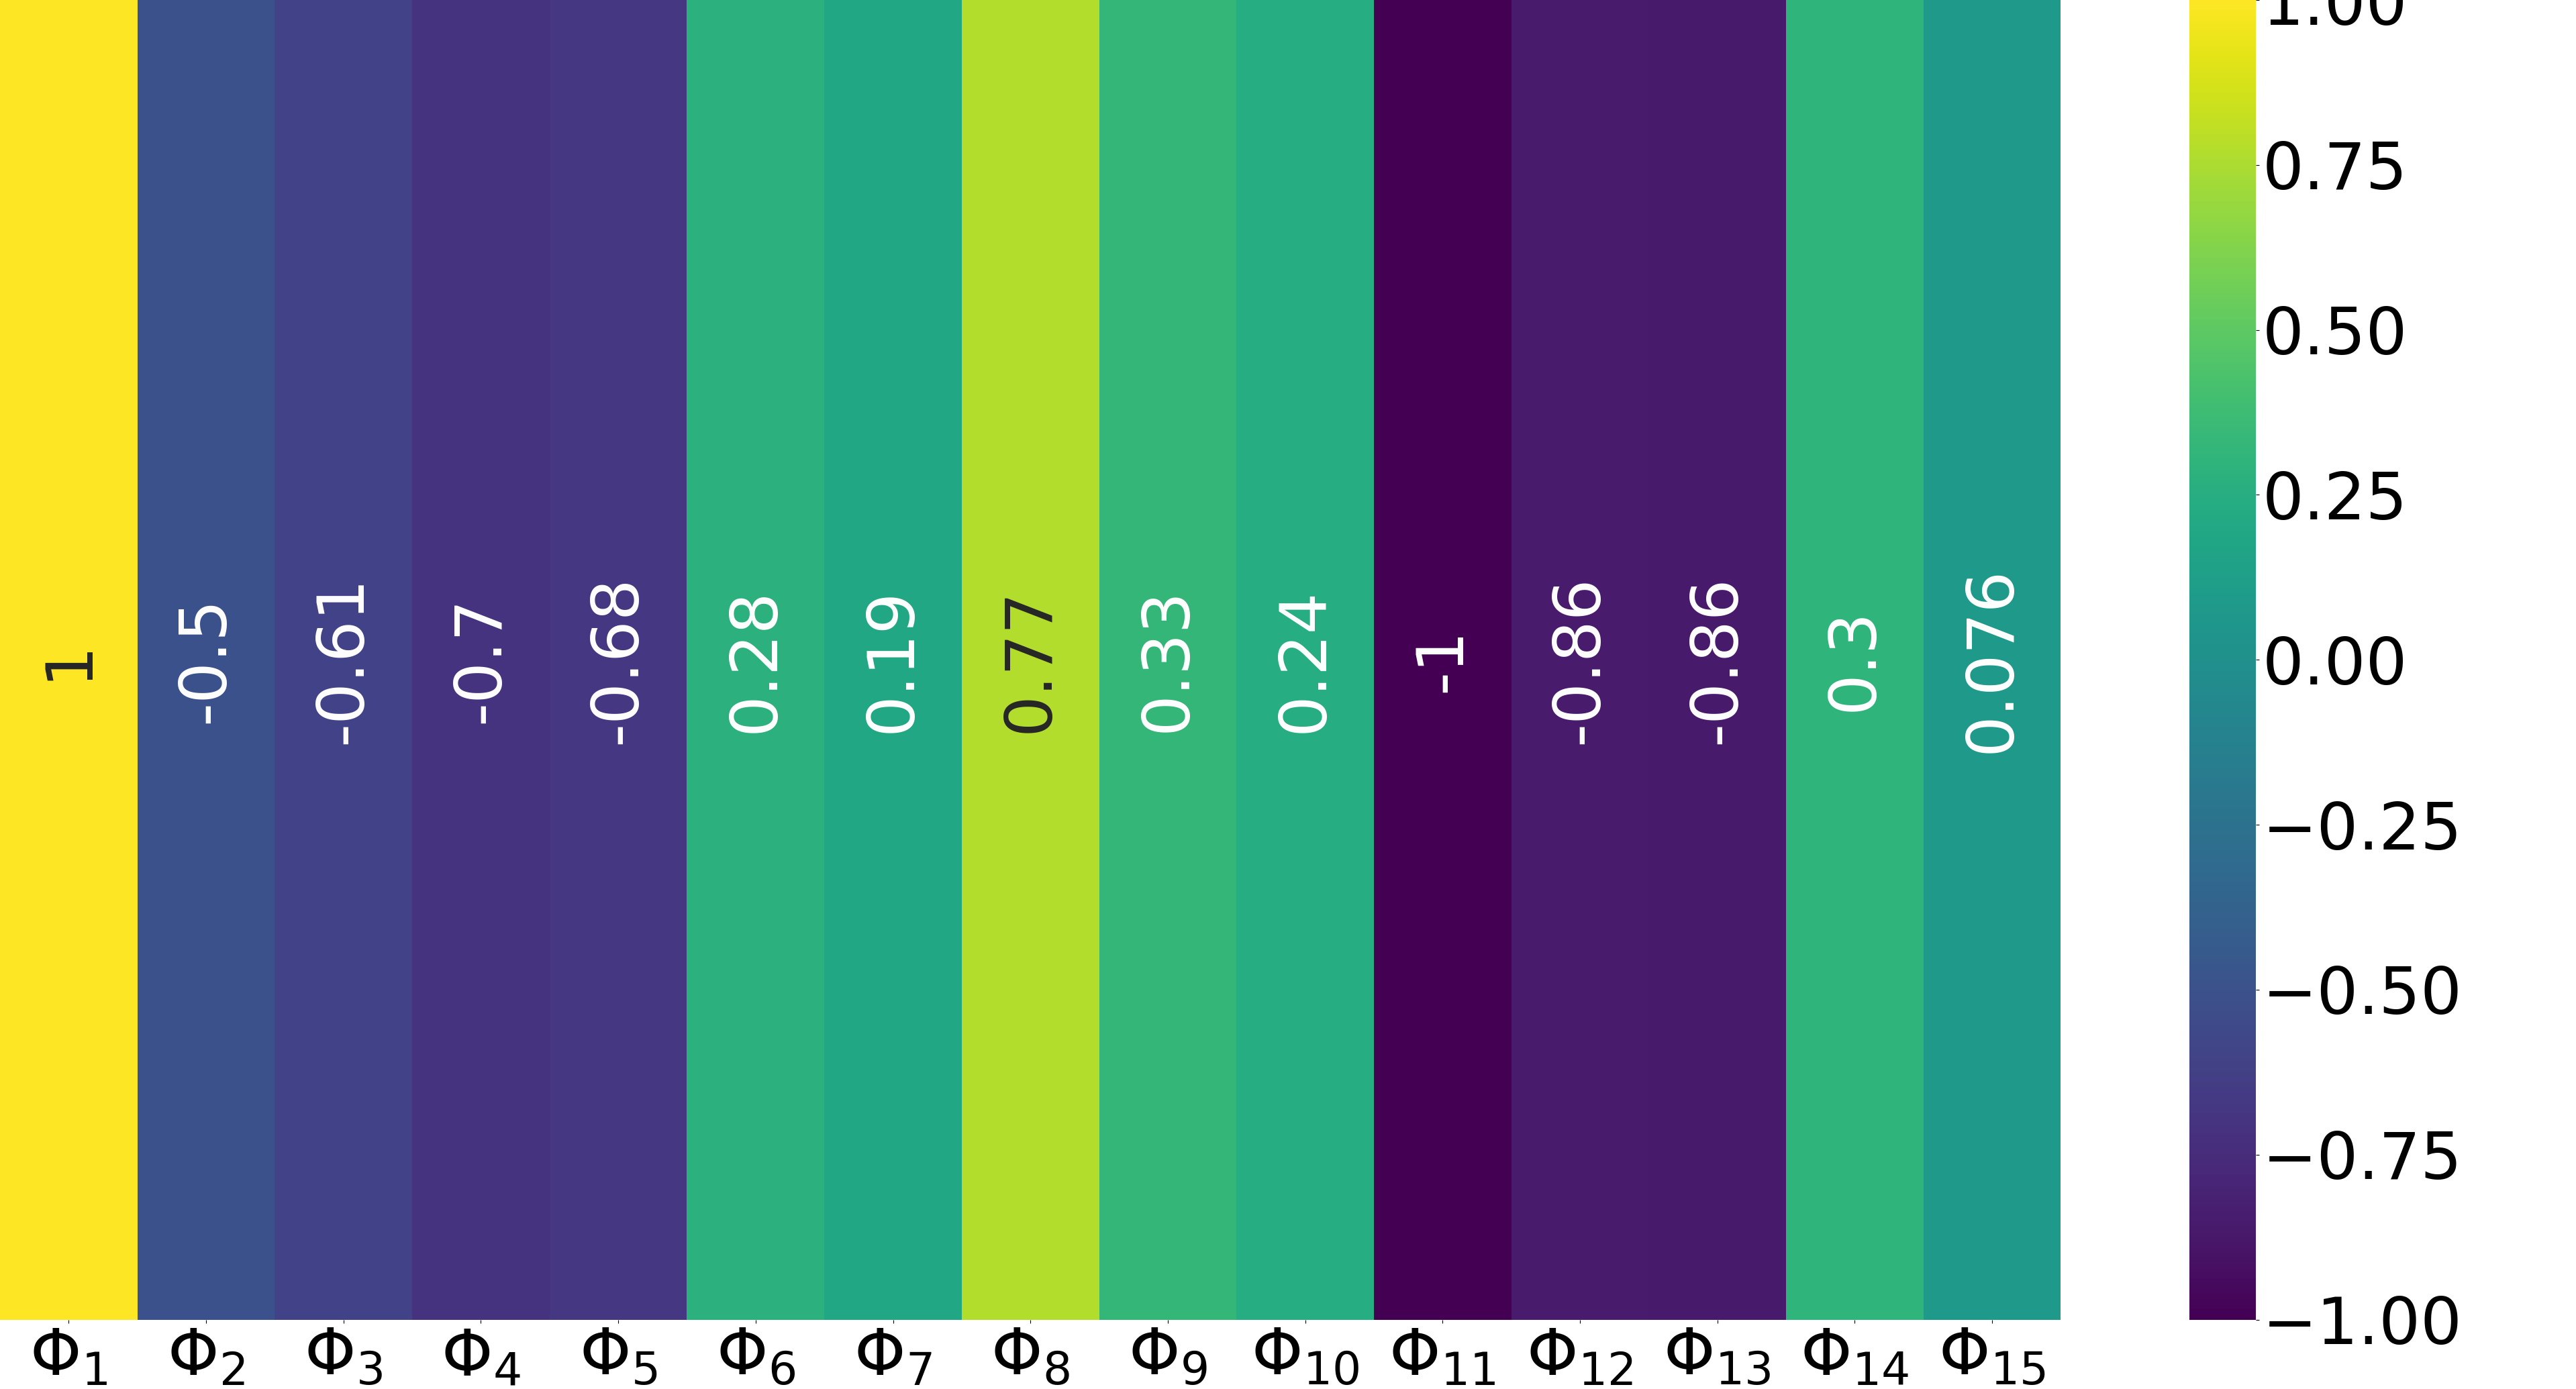
\includegraphics[width=\linewidth]{img/qlp_corr/Phi_coil0.png}
		\subcaption{Correlation with coil $0$}
	\end{subfigure}
	\begin{subfigure}{0.49\linewidth}
		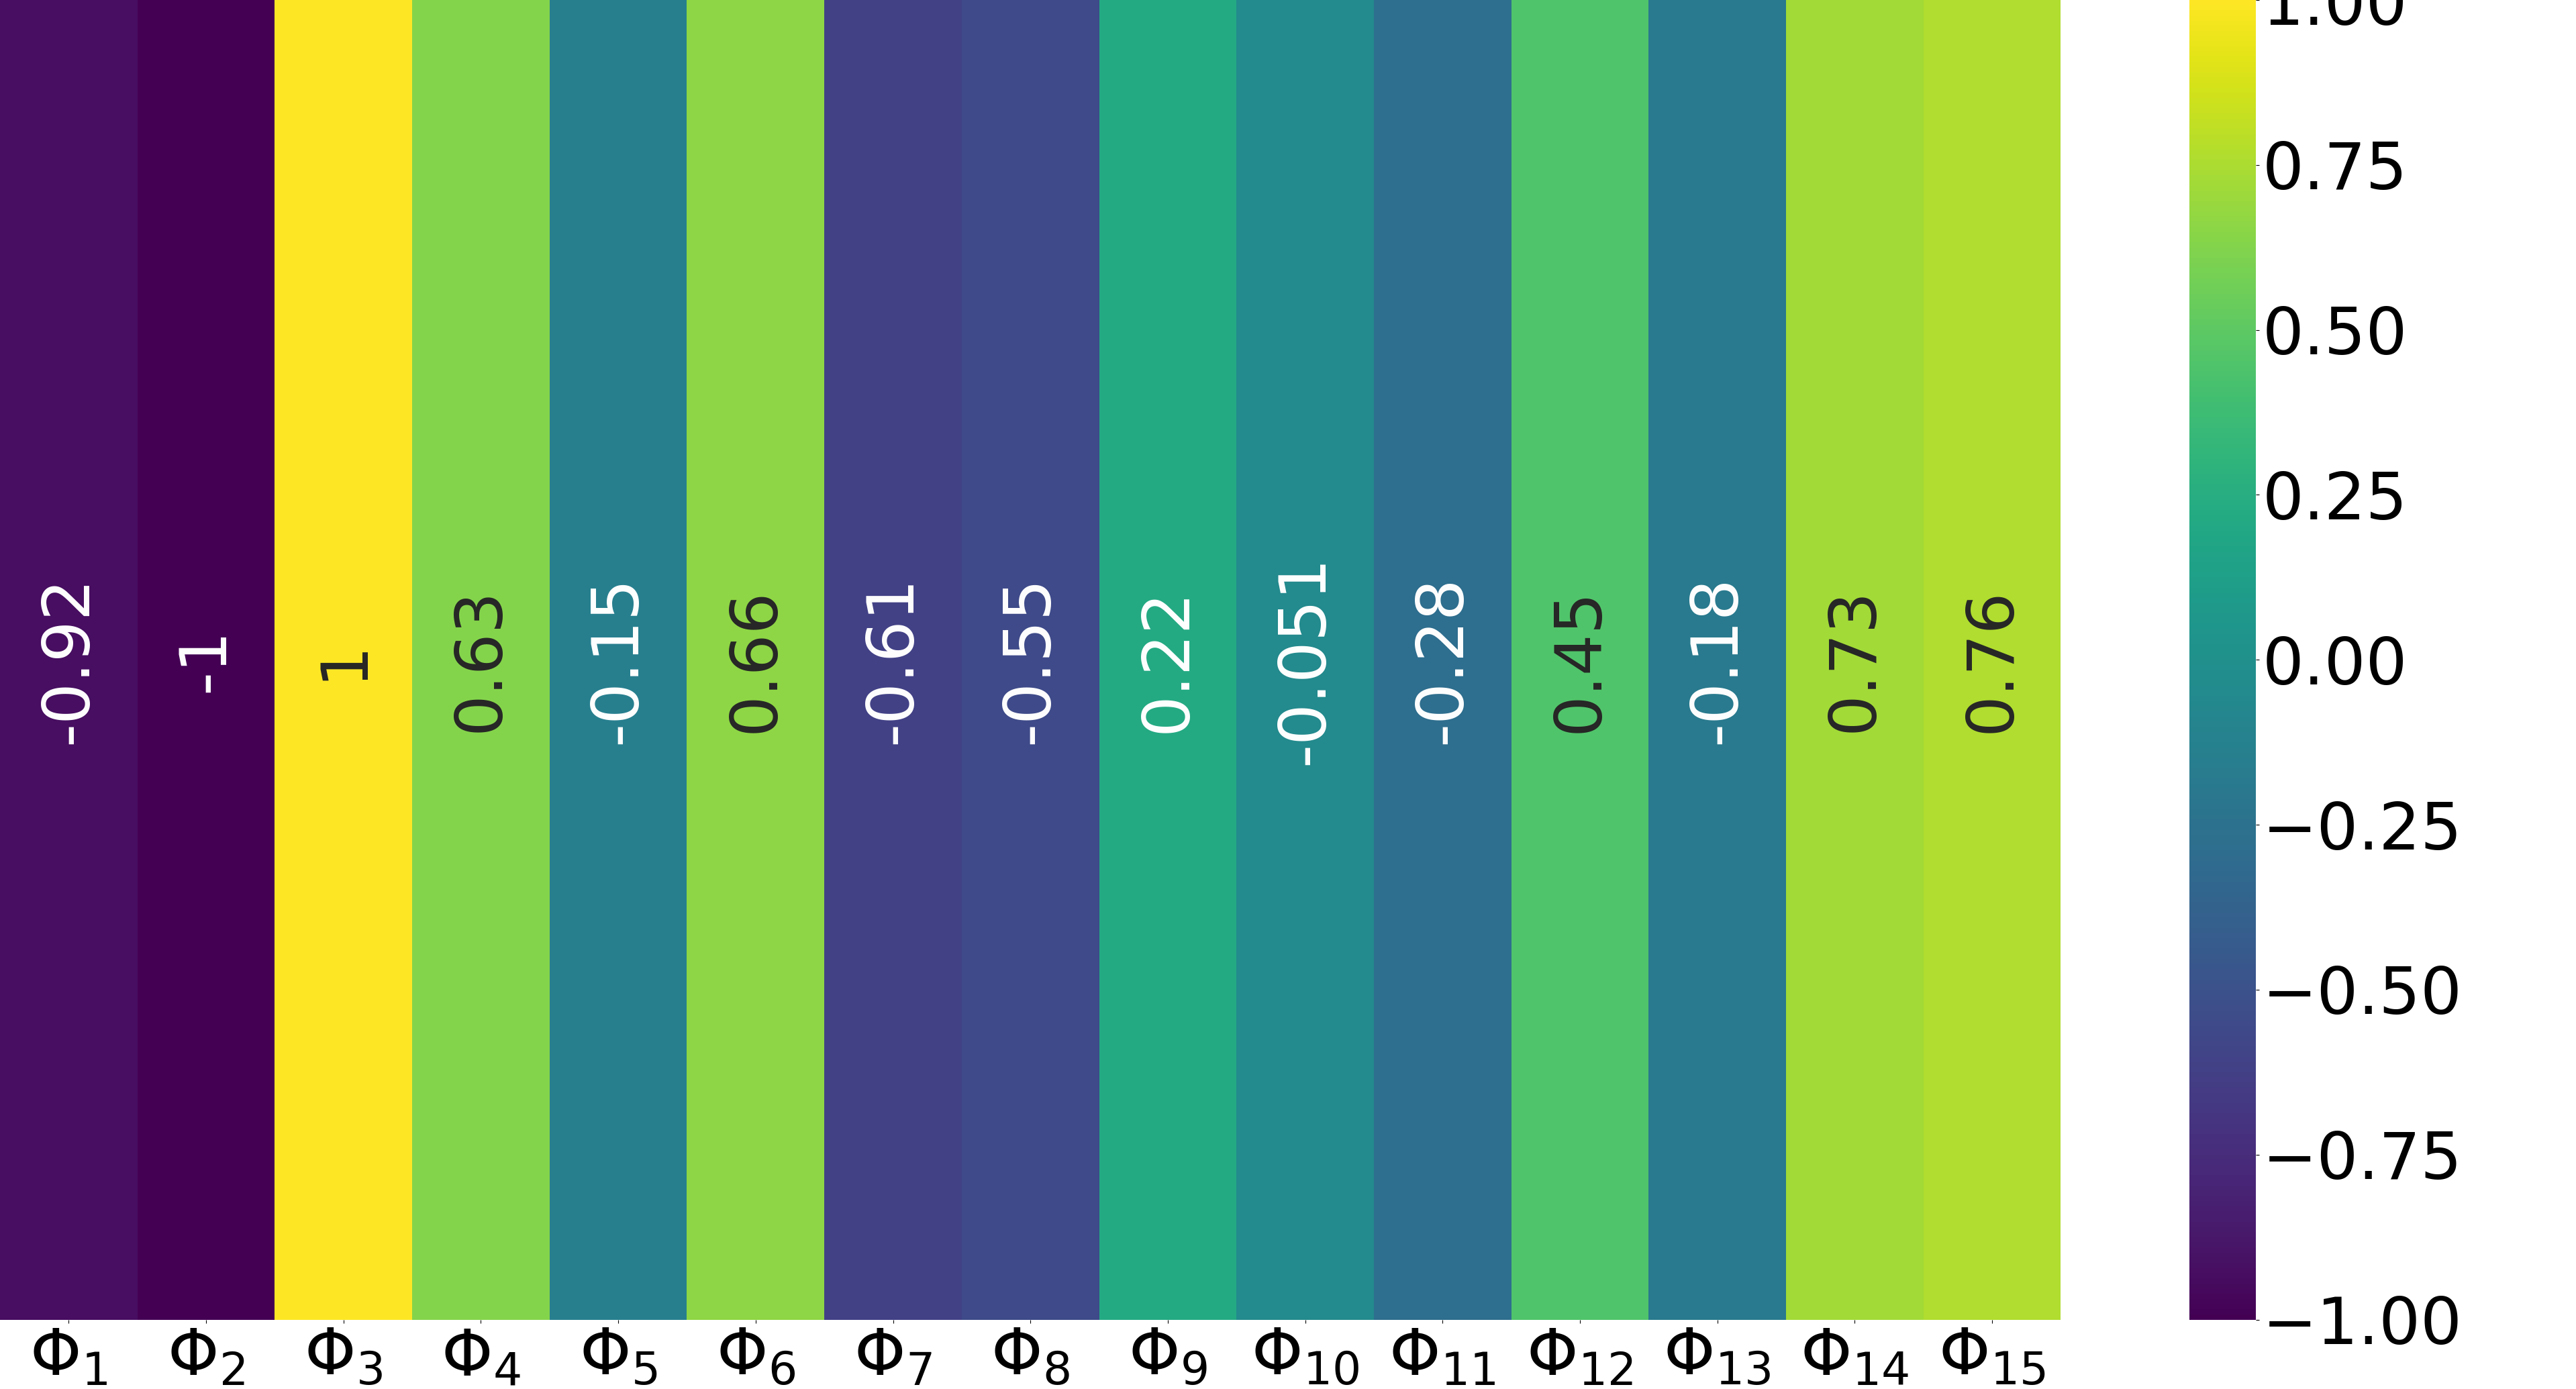
\includegraphics[width=\linewidth]{img/qlp_corr/Phi_coil1.png}
		\subcaption{Correlation with coil $1$}
	\end{subfigure}
	\begin{subfigure}{0.49\linewidth}
		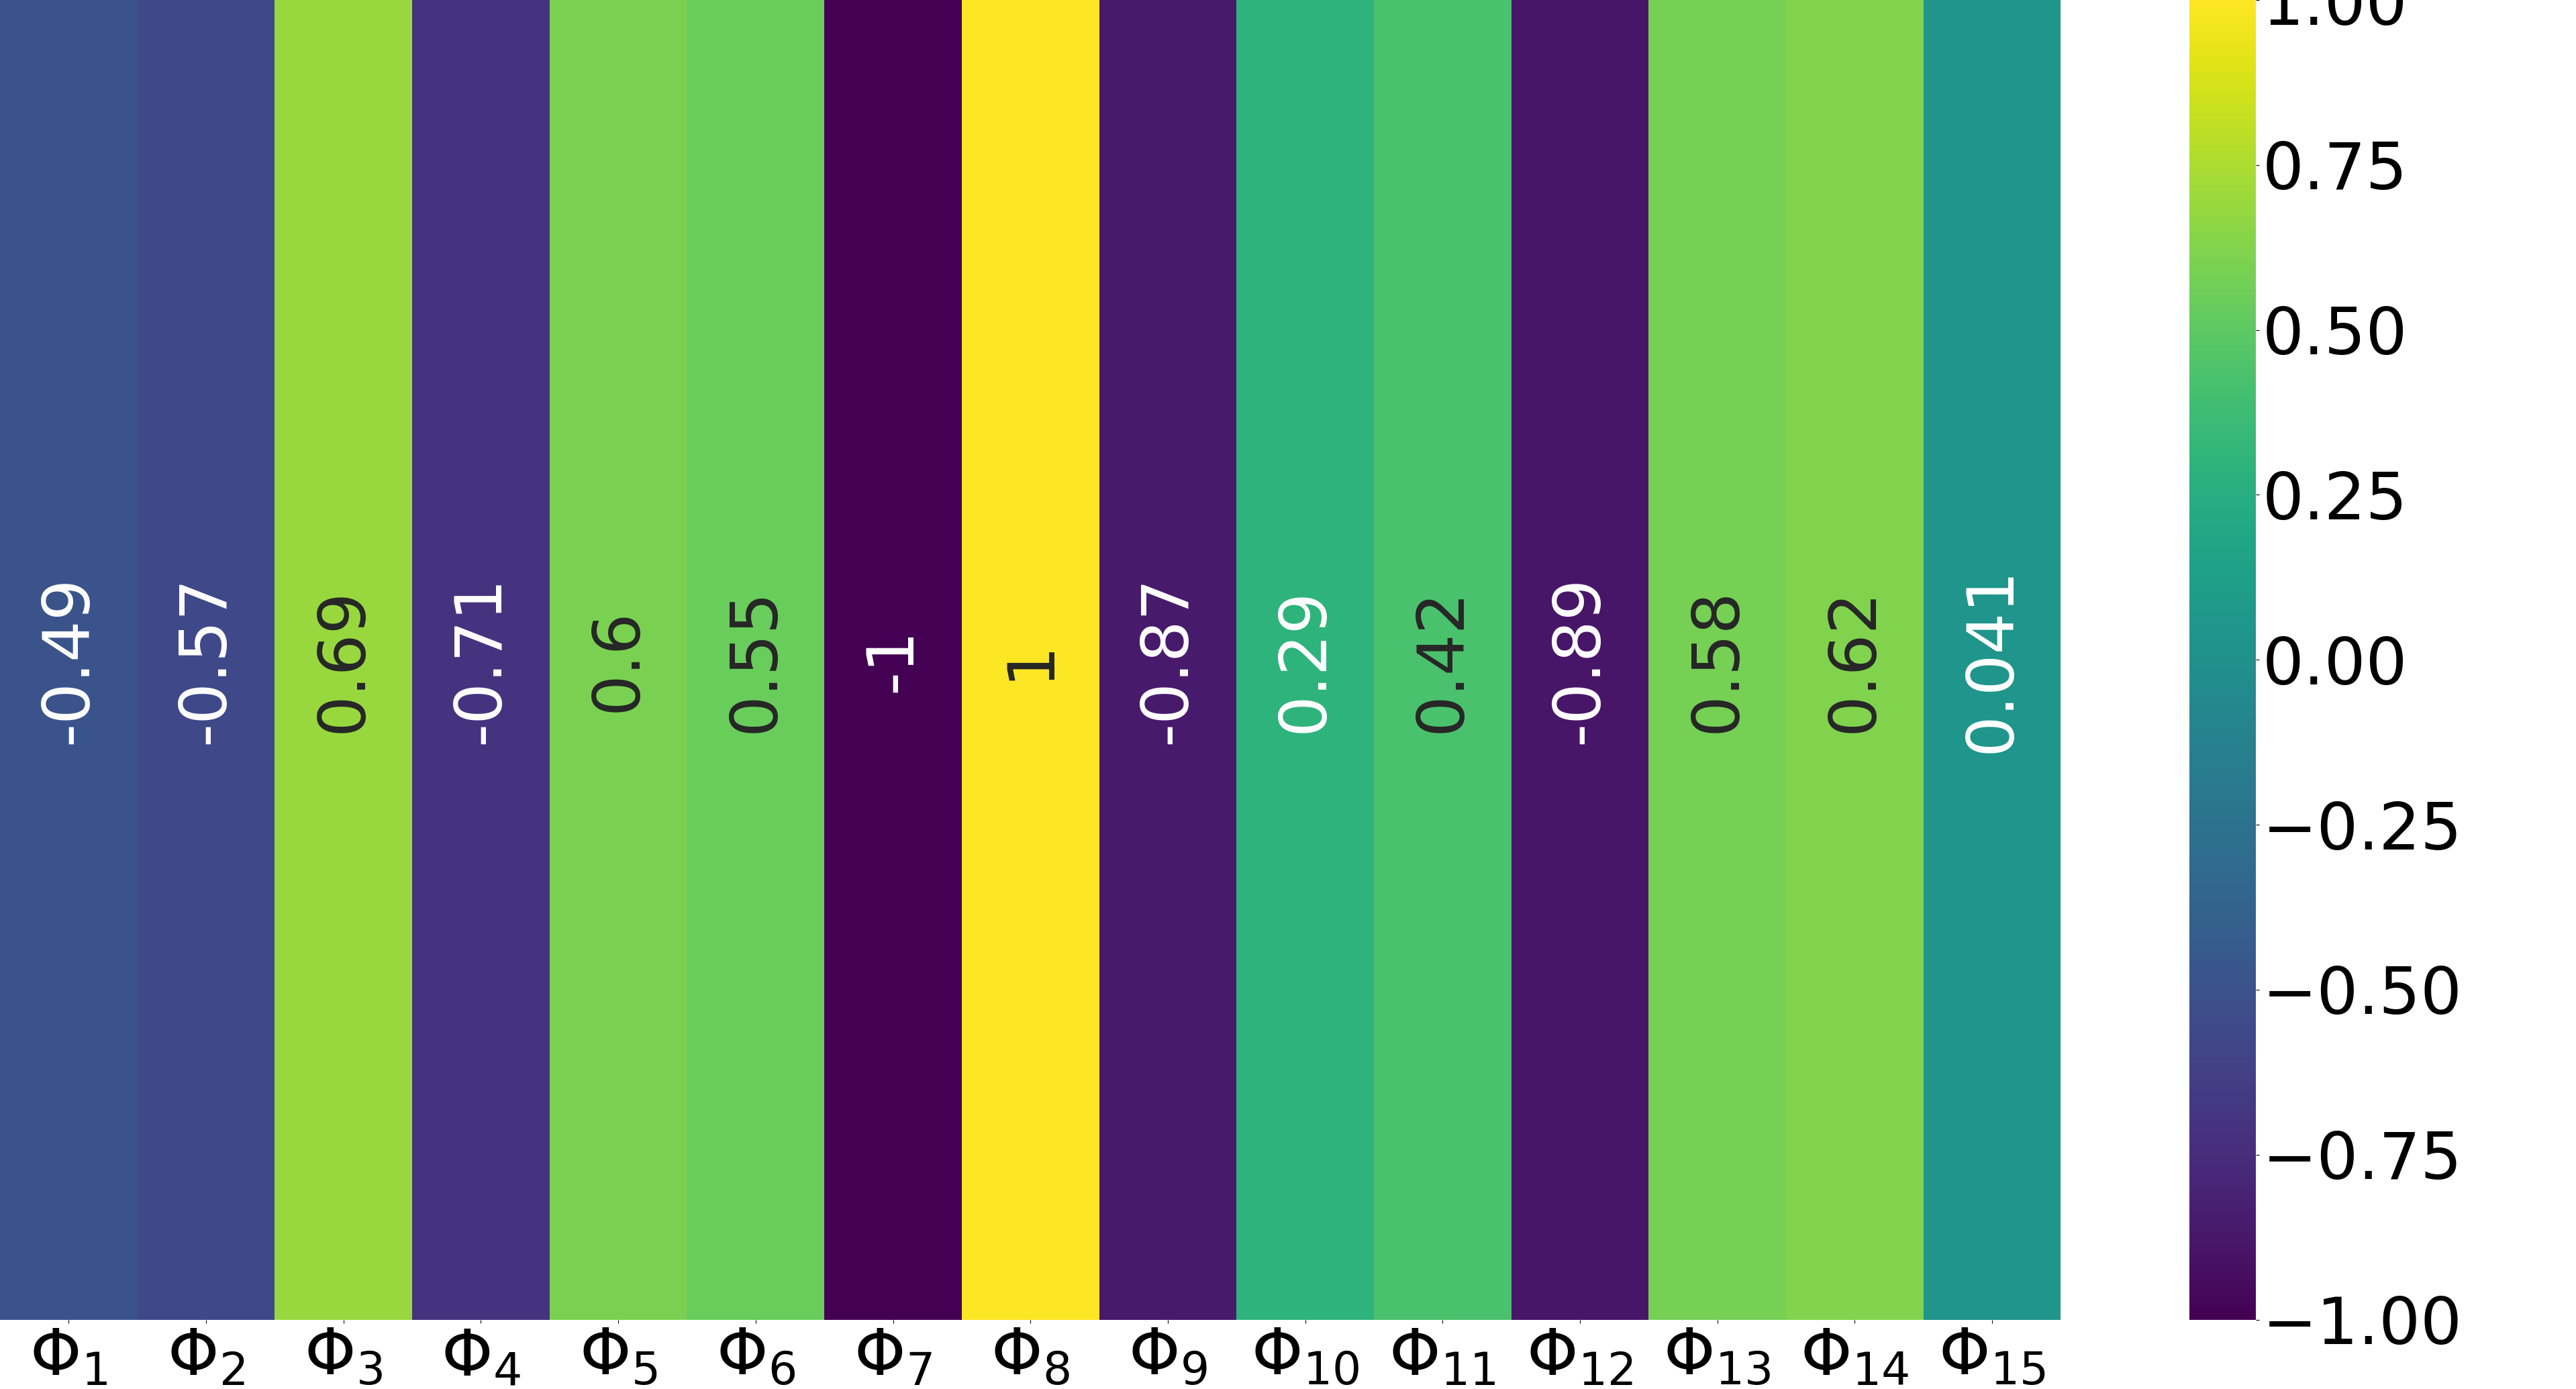
\includegraphics[width=\linewidth]{img/qlp_corr/Phi_coil2.png}
		\subcaption{Correlation with coil $2$}
	\end{subfigure}
	\begin{subfigure}{0.49\linewidth}
		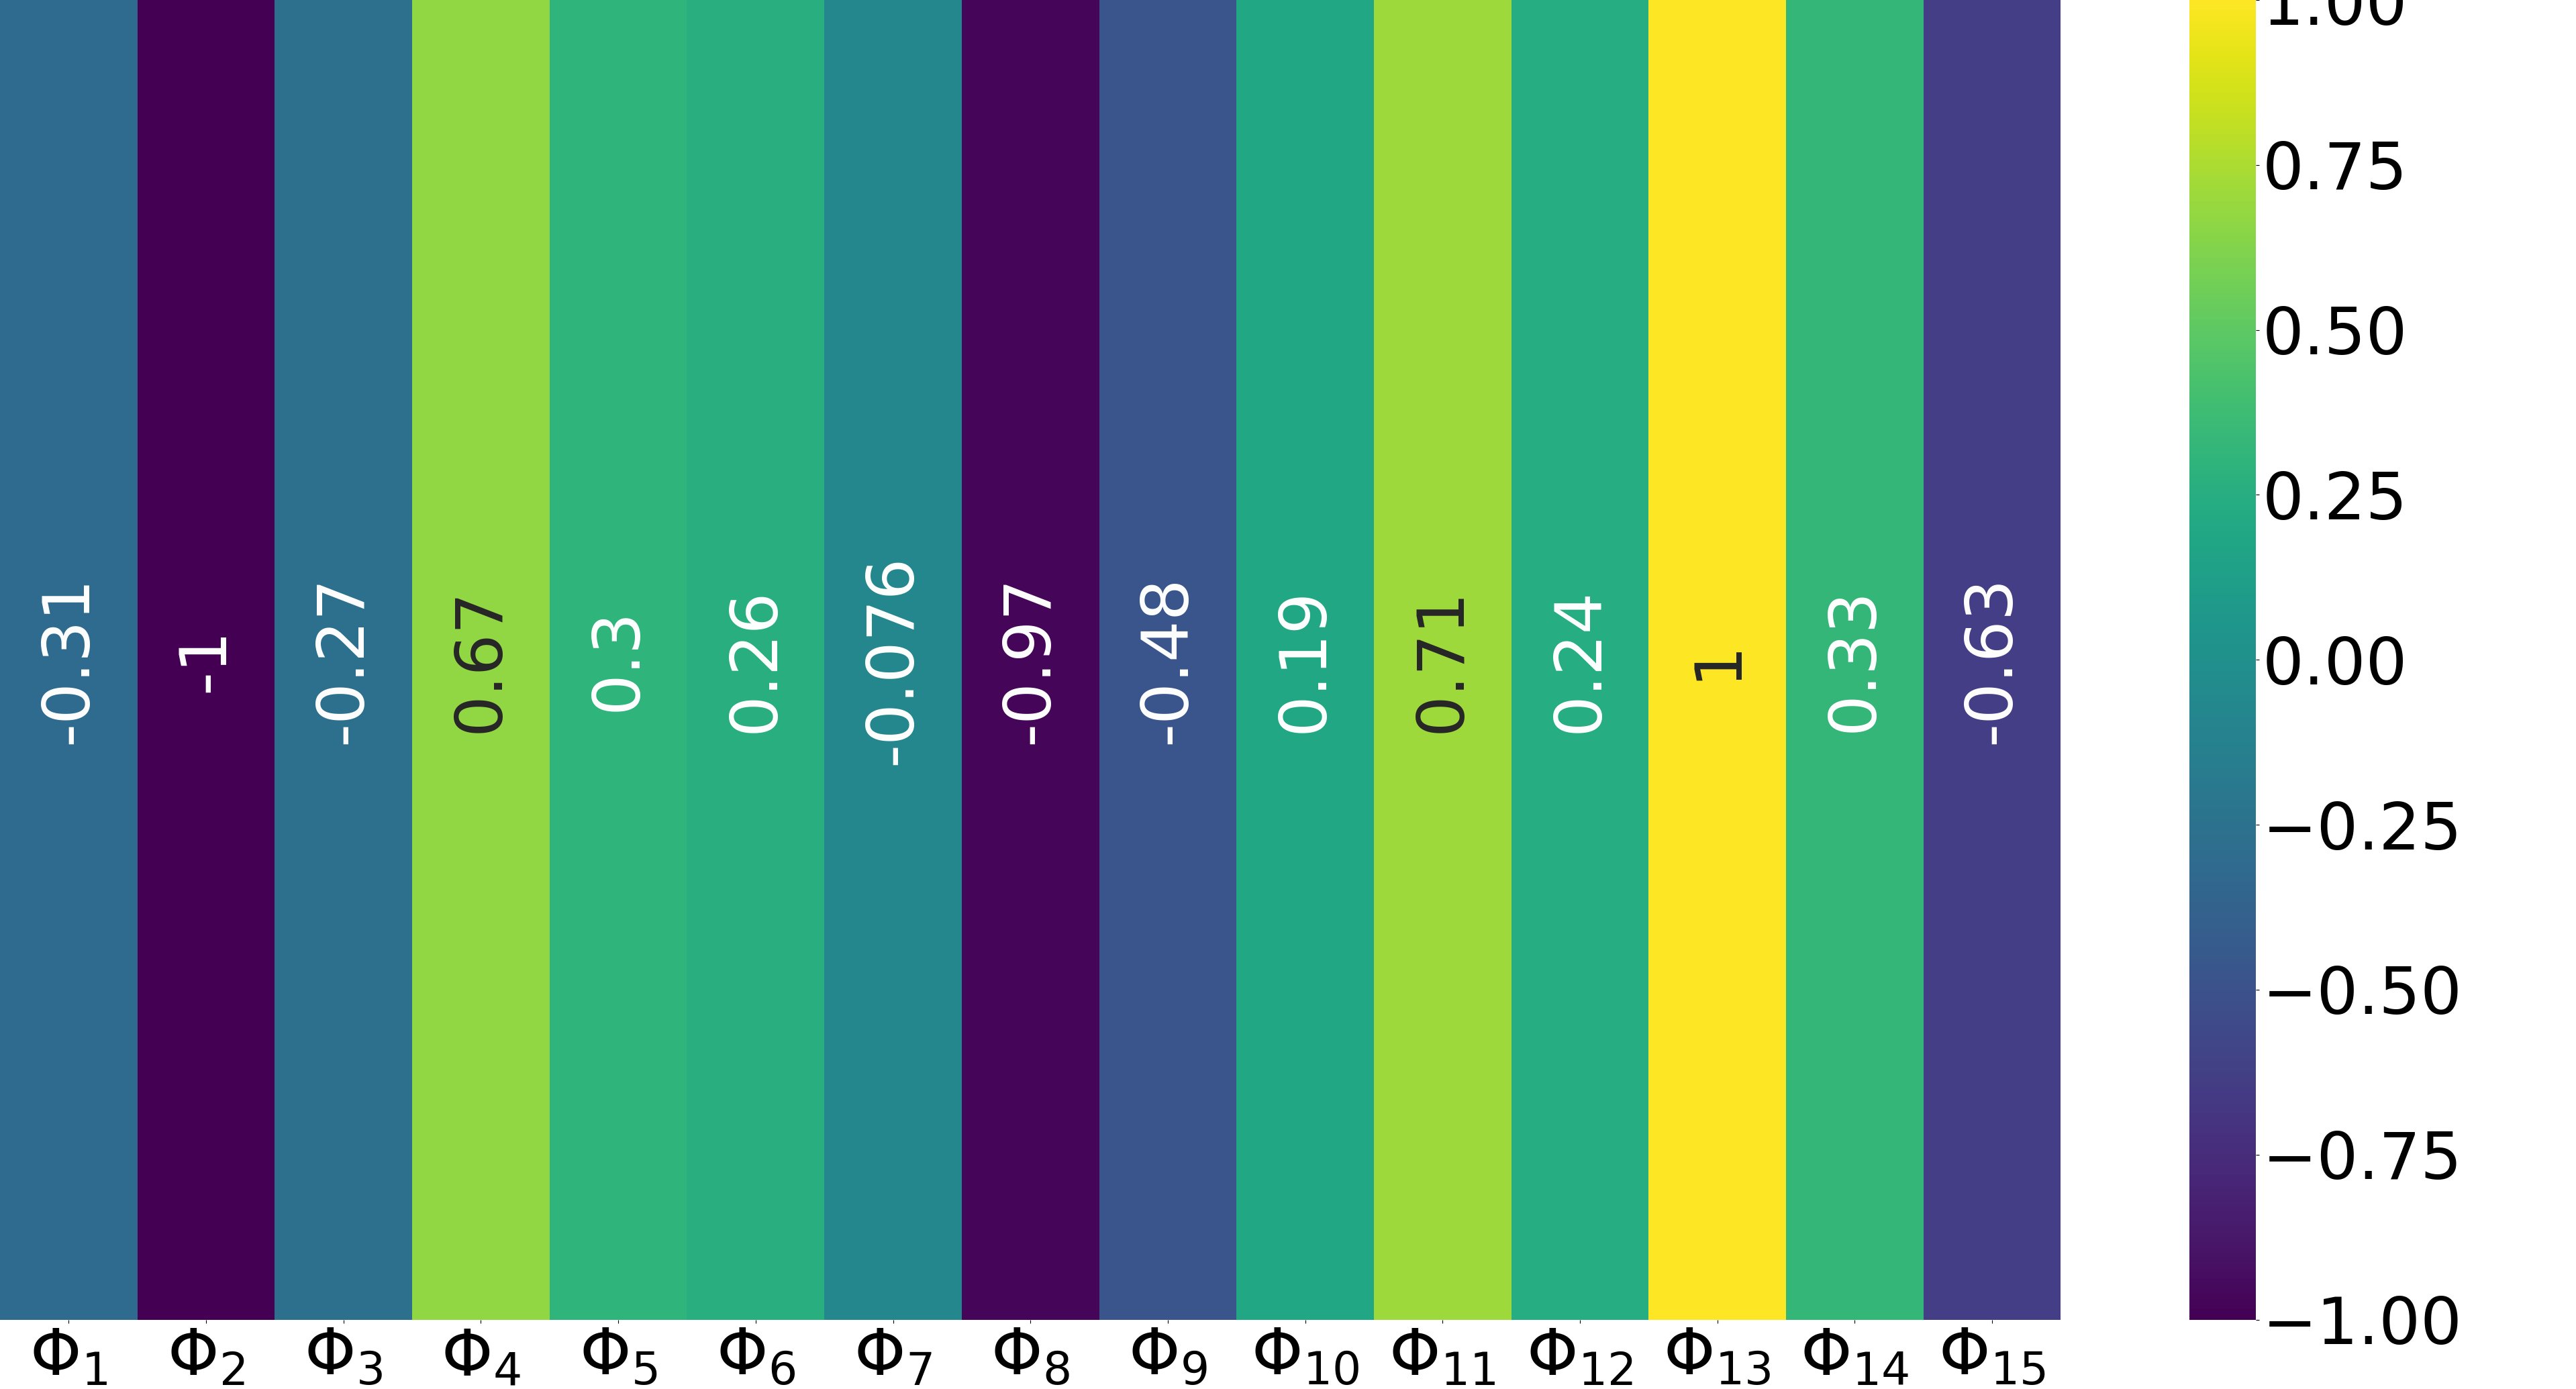
\includegraphics[width=\linewidth]{img/qlp_corr/Phi_coil3.png}
		\subcaption{Correlation with coil $3$}
	\end{subfigure}
	\caption{Correlation between the harmonics of the \phin\ attribute and the labels for \qlp.}
	\label{fig:phi-lcorr-qlp}
\end{figure}

\begin{figure}[!ht]
	% Font size = 40
	\centering
	\begin{subfigure}{0.8\linewidth}
		\centering
		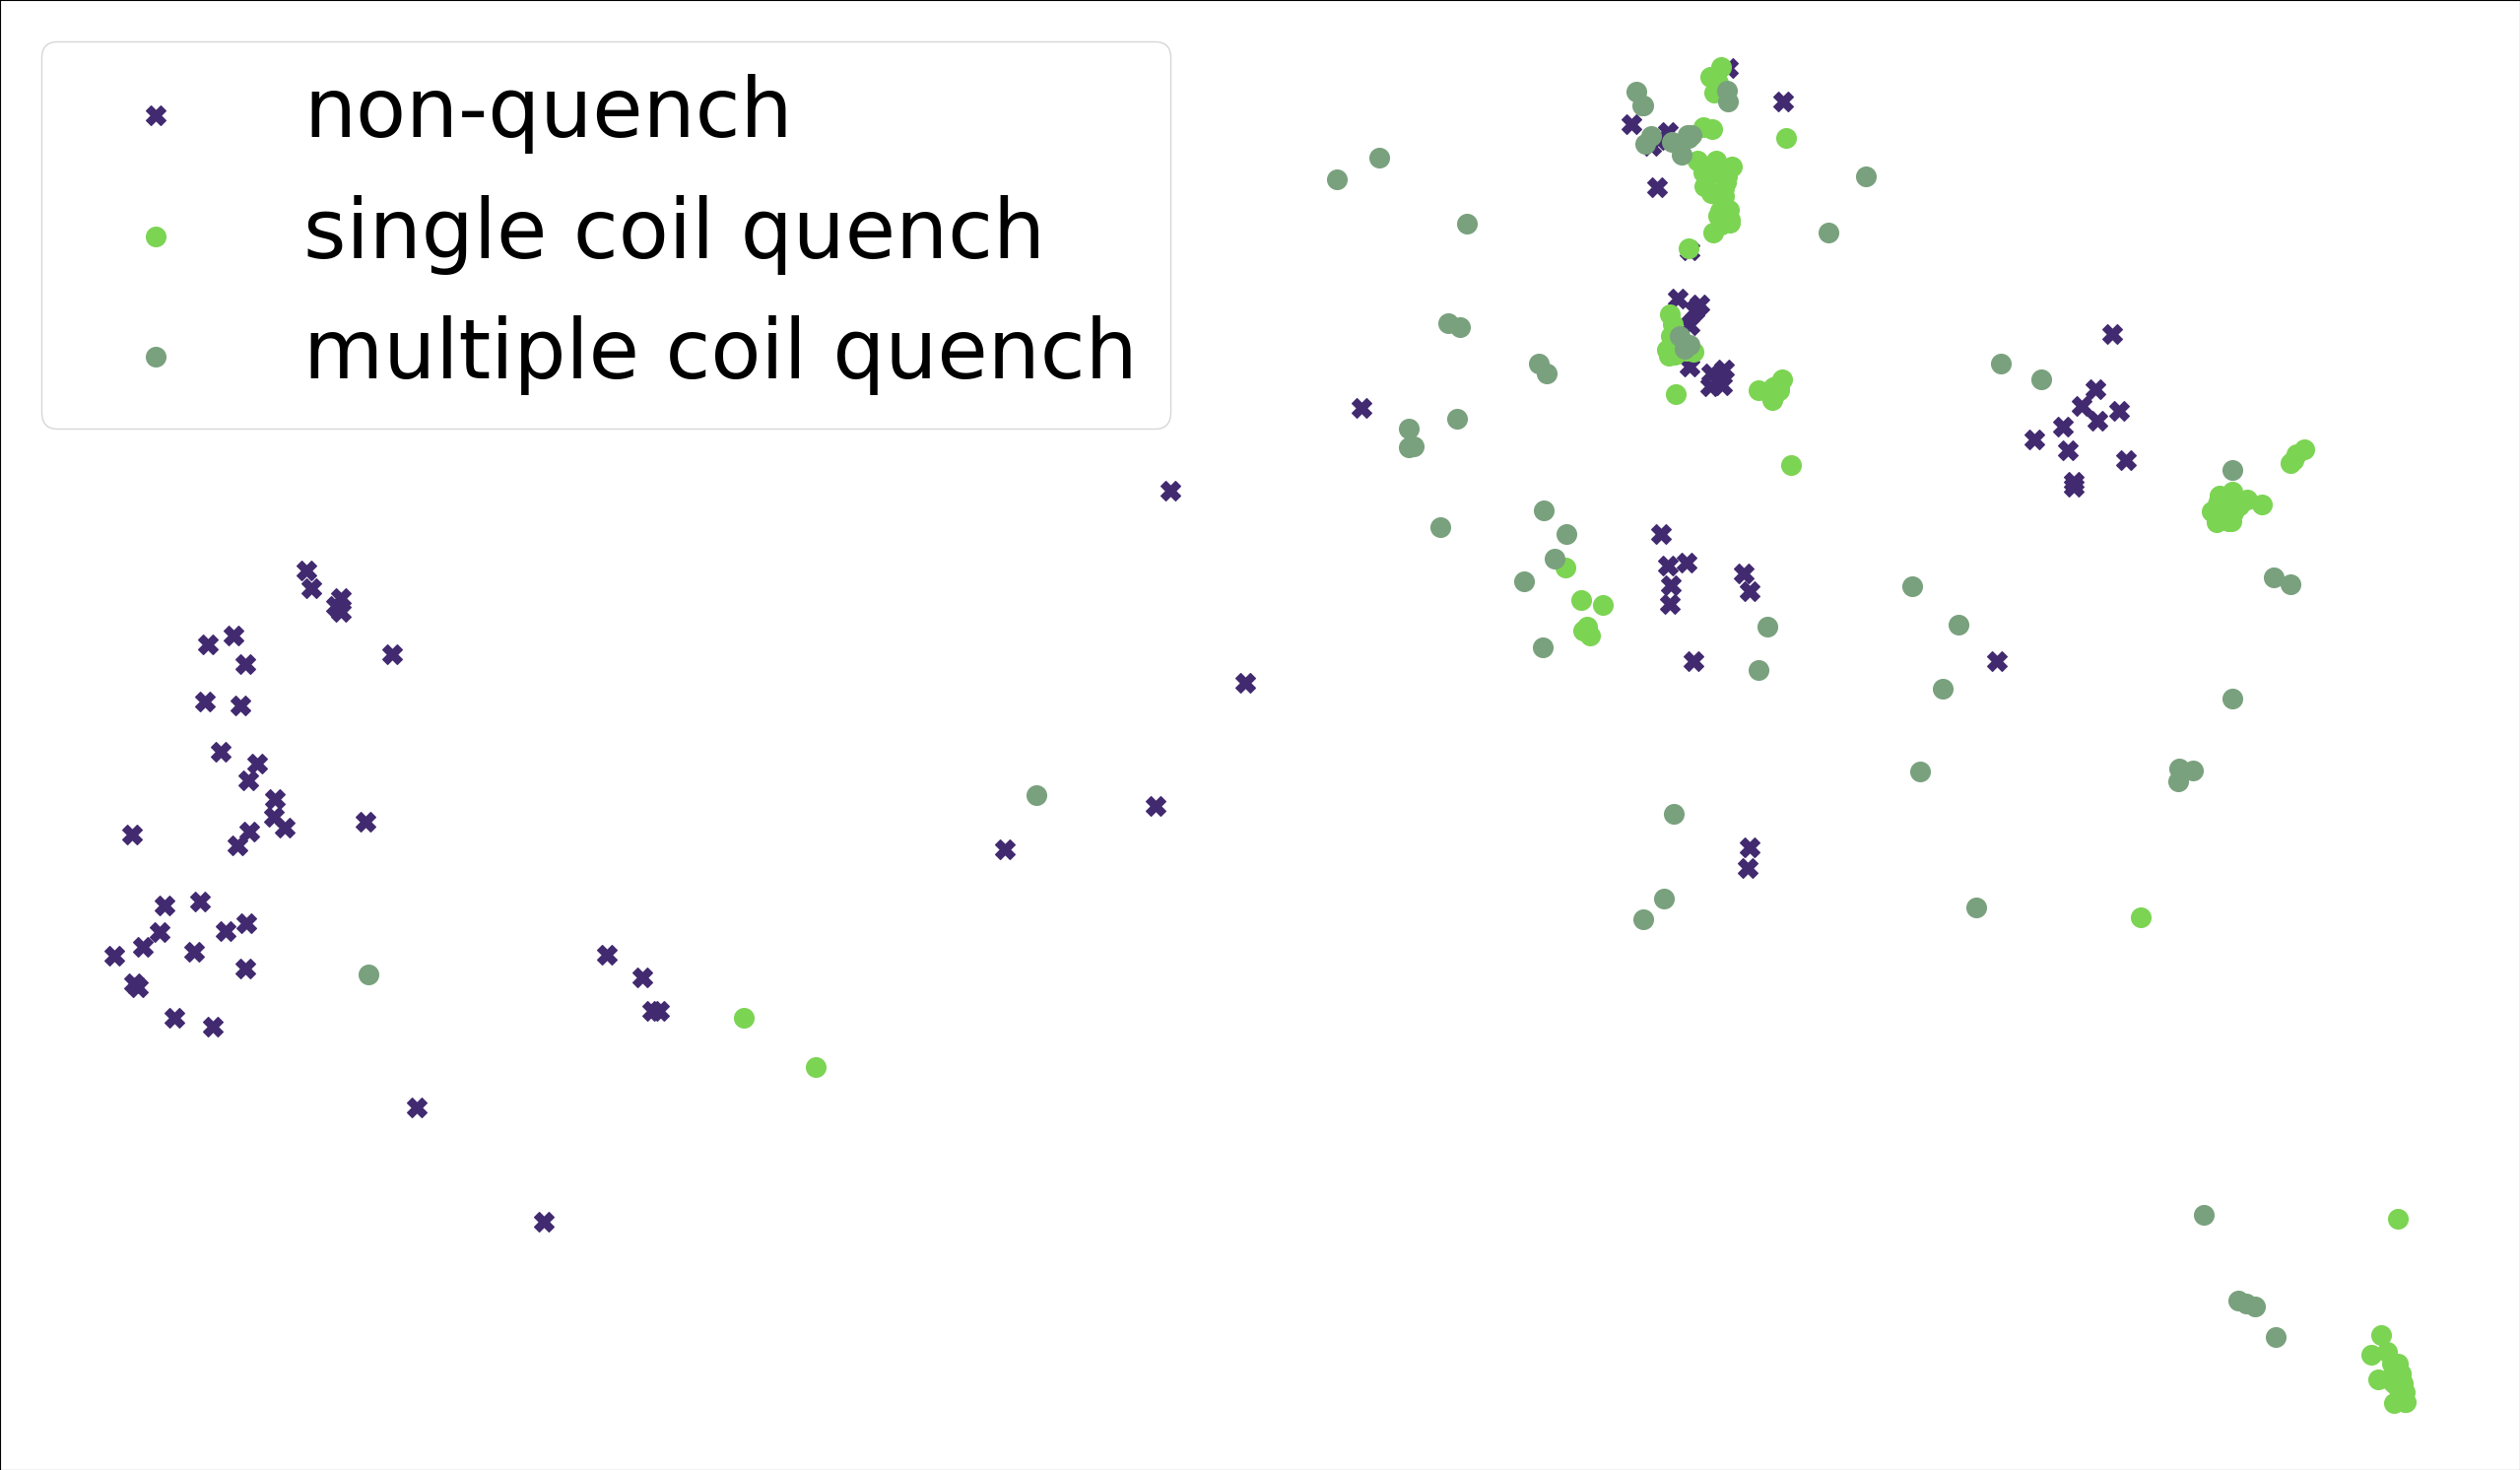
\includegraphics[width=\linewidth]{img/quench_dist_qlp/single_vs_multiple_Phi.png}
		\subcaption{}
	\end{subfigure}
	\begin{subfigure}{0.8\linewidth}
		\centering
		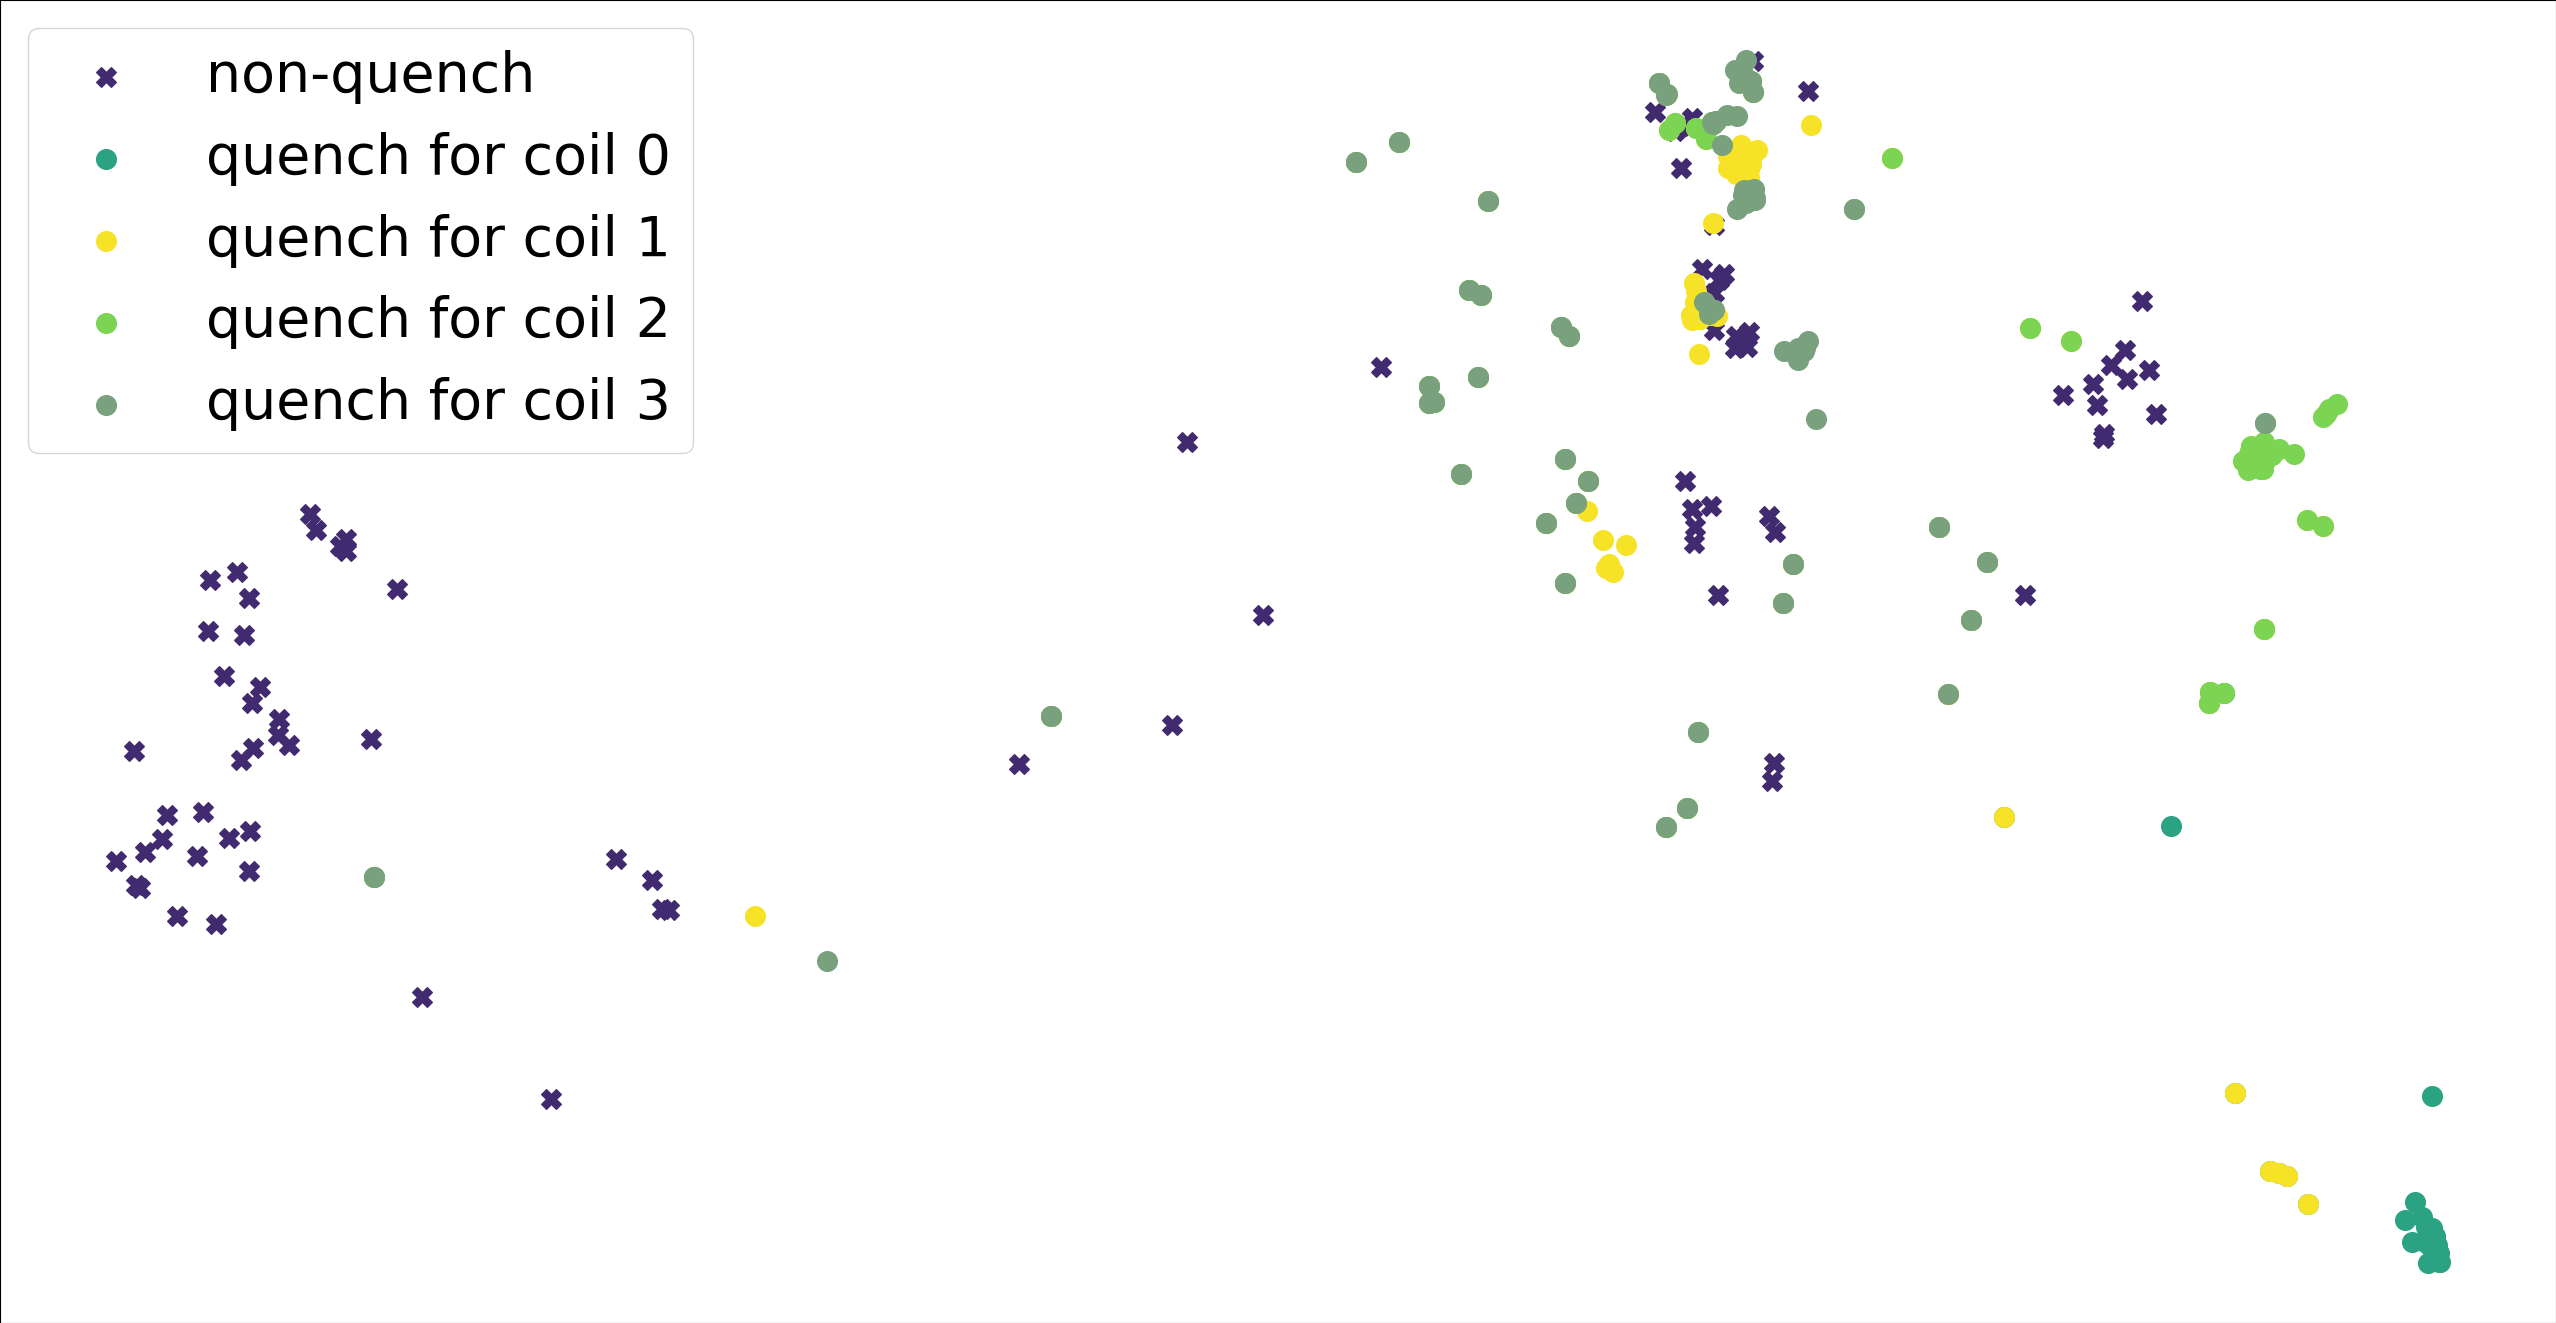
\includegraphics[width=\linewidth]{img/quench_dist_qlp_phi.png}
		\subcaption{}
	\end{subfigure}
	\caption{Visualization of the \phin\ attribute, the data was plotted after a run of \pca\
		dimensionality reduction. Sub-figure (a) highlights the samples based on how many quenches
		are associated to the specific sample $\{0, 1, \text{many}\}$. Sub-figure (b) highlights the
		samples based on the specific coil quenched $\{\text{None}, 0, 1, 2, 3\}$.}
	\label{fig:phi-coilq-dist}
\end{figure}

\section{First approaches using Clustering}
\label{sec:qlp-cluster}
We initially discovered that \an\ and \cnmod\ data was scattered favorably in bidimensional space
while we were still studying \qrp. We had the idea to use clustering because it was unsupervised,
and we wanted to understand if there was a way for us to get very early results in \qlp\ by
leveraging some undiscovered patterns in the data.

We remark that the clustering algorithm is always working by using distance between samples,
therefore the pattern that it's capable of identifying is unknown to us, and we, as researchers,
have to identify it. Even if we applied clustering to all the attributes in the following we will
only bother to show the results obtained for \an\ and \cnmod\ since they are the more promising.
Data was plotted using \pca, but we also used other dimensionality reduction techniques, generally
with inferior results.

We tried to achieve similar results using \cnmod, but the data seems to be too homogeneously
distributed in some cases, leading to the generation of clusters that are not splitting data that
actually belong to different classes. Clustering-specific performance (originally introduced in
\Cref{chp:ml}) actually tell us that the best results were obtained when we built $4$ clusters on
both \an\ and \cnmod. \Cref{fig:4-means-results} shows the results for the \an\ and \cnmod\
attributes after a run of $4$-means clustering, we chose to highlight the labels of single and
multiple coil quench. In the picture the orange lines represent the borders
of the clusters, if the line is solid then the cluster has a finite size, otherwise the cluster has
infinite size.

While the result for \an\ (subfigure (a)) contains $3$ clusters that essentially have a high degree
of purity (the top for the magnet in normal operating conditions, the left and right for quench
events). The central cluster mixes quench and non-quench data, making it less useful for our
classification needs. If we consider \cnmod (subfigure (b)), while it's far from perfect, we can see
that the clusters have a decent level of purity since each cluster contains, essentially, a majority
of samples coming from a specific class (in the case of quench and non-quench classification).
\begin{figure}[!ht]
	\centering
	\begin{subfigure}{0.8\linewidth}
		\centering
		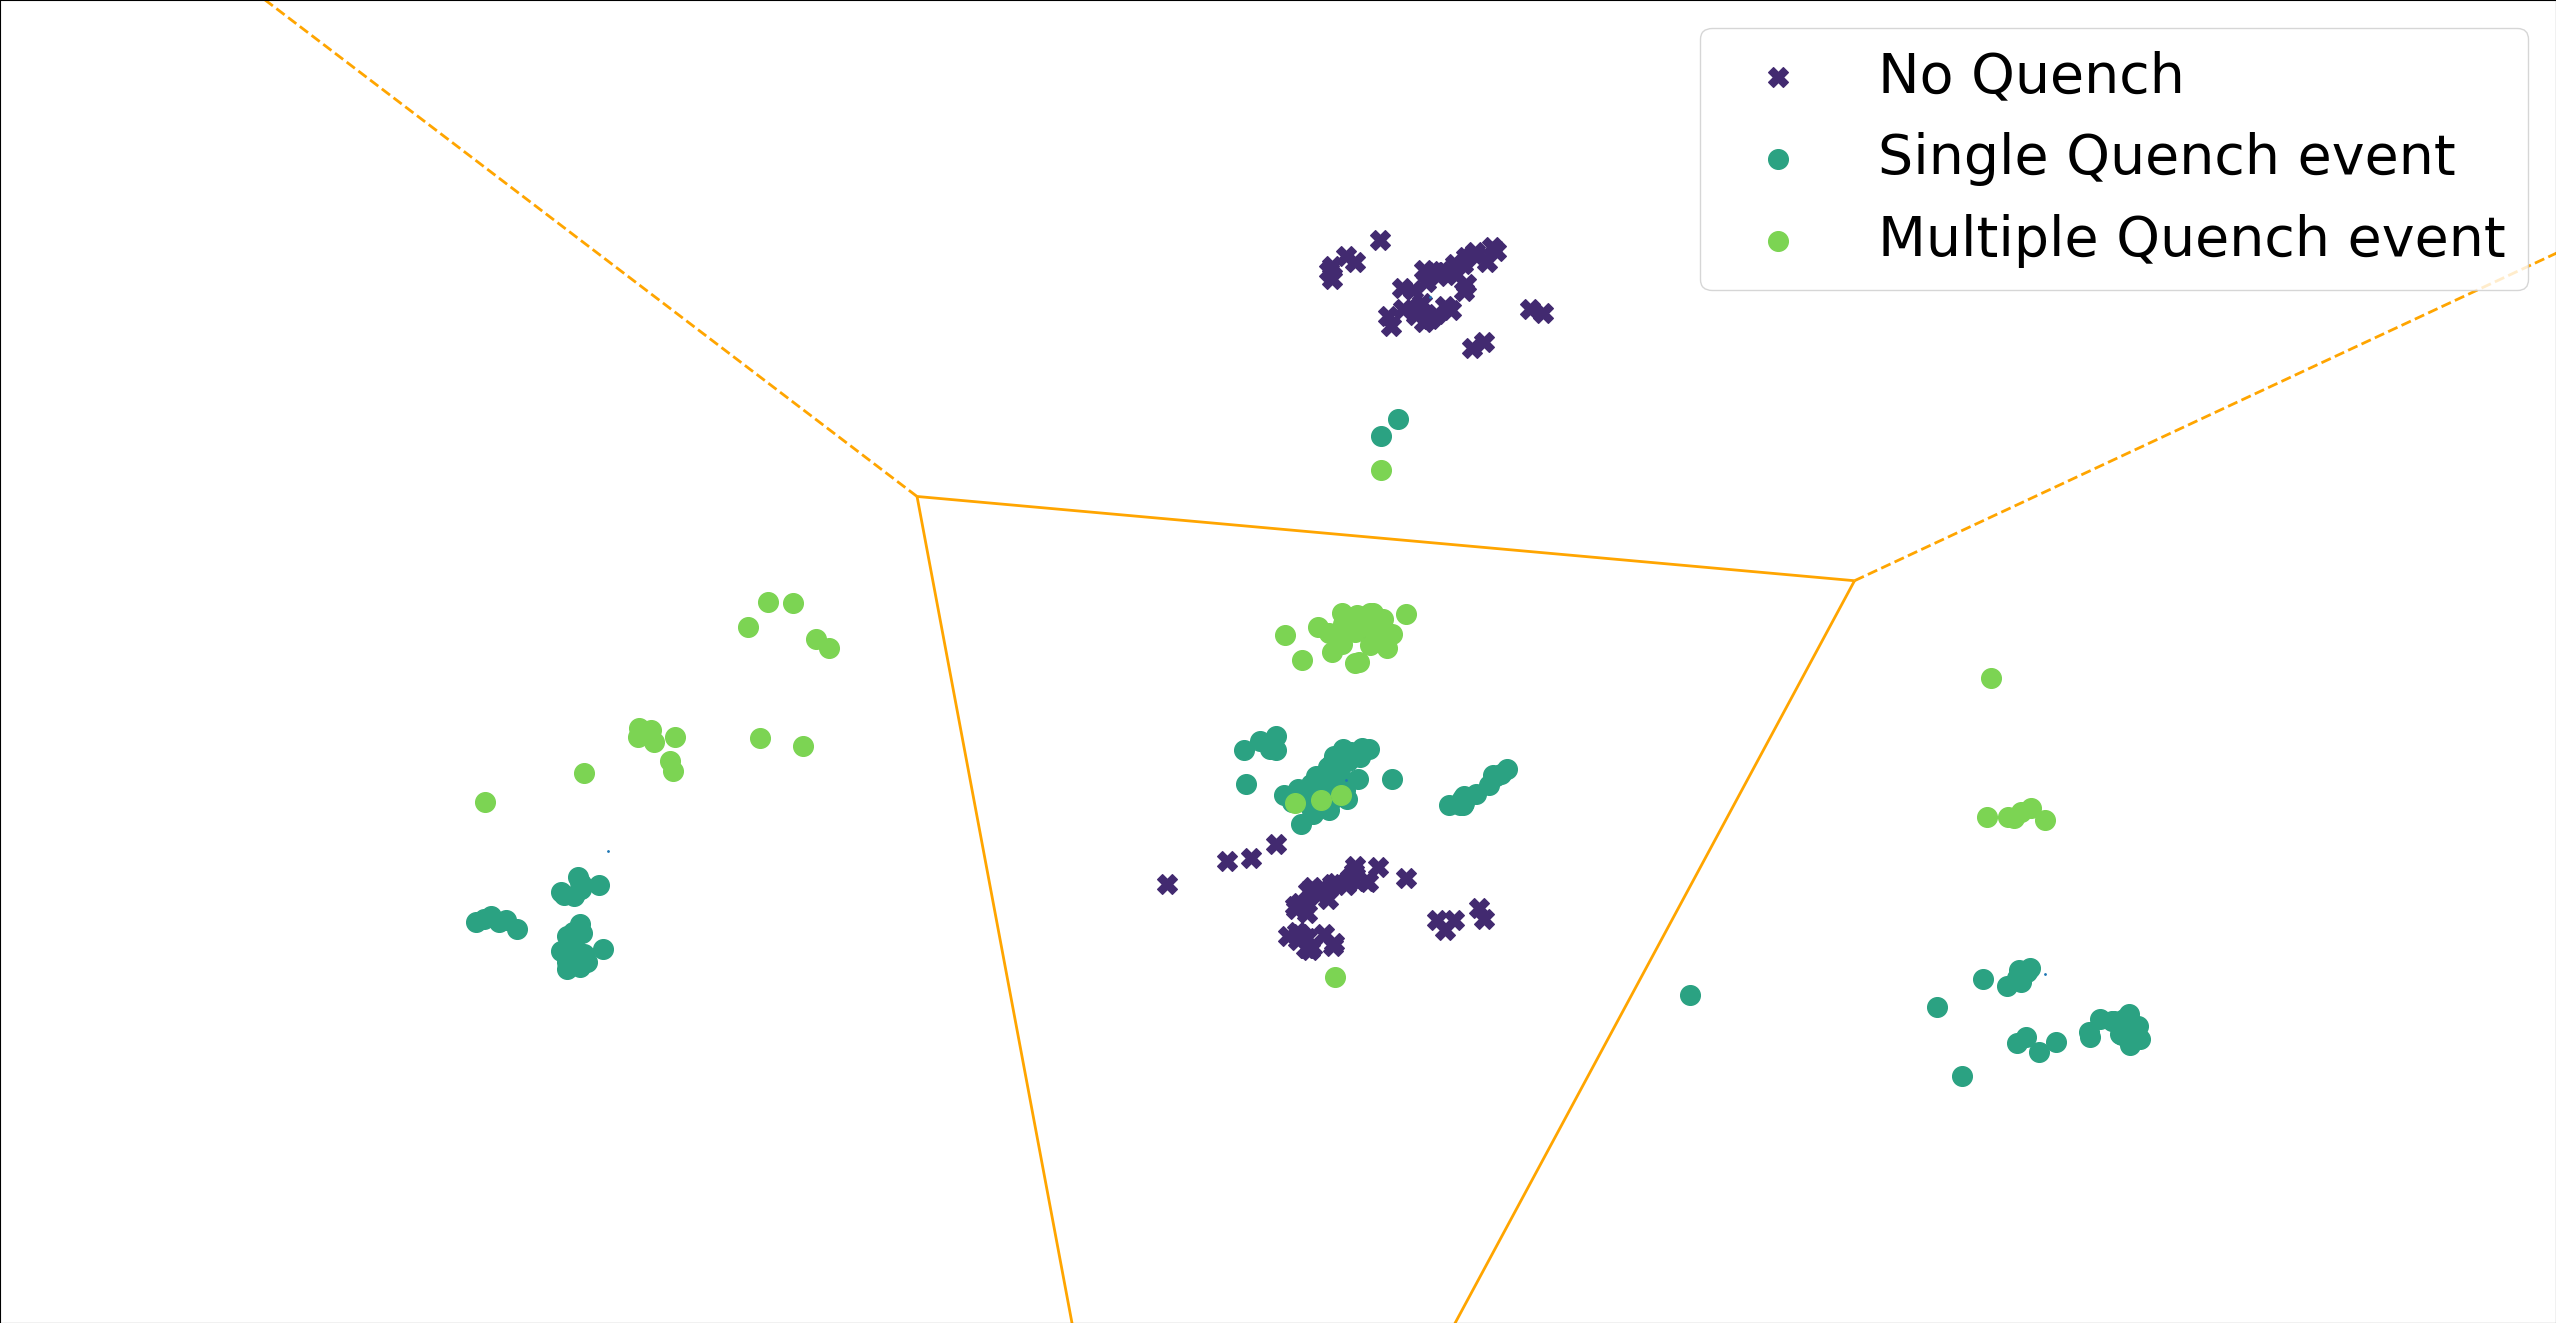
\includegraphics[width=\linewidth]{img/clustering_an_qlp_4c.png}
		\caption{}
	\end{subfigure}
	\begin{subfigure}{0.8\linewidth}
		\centering
		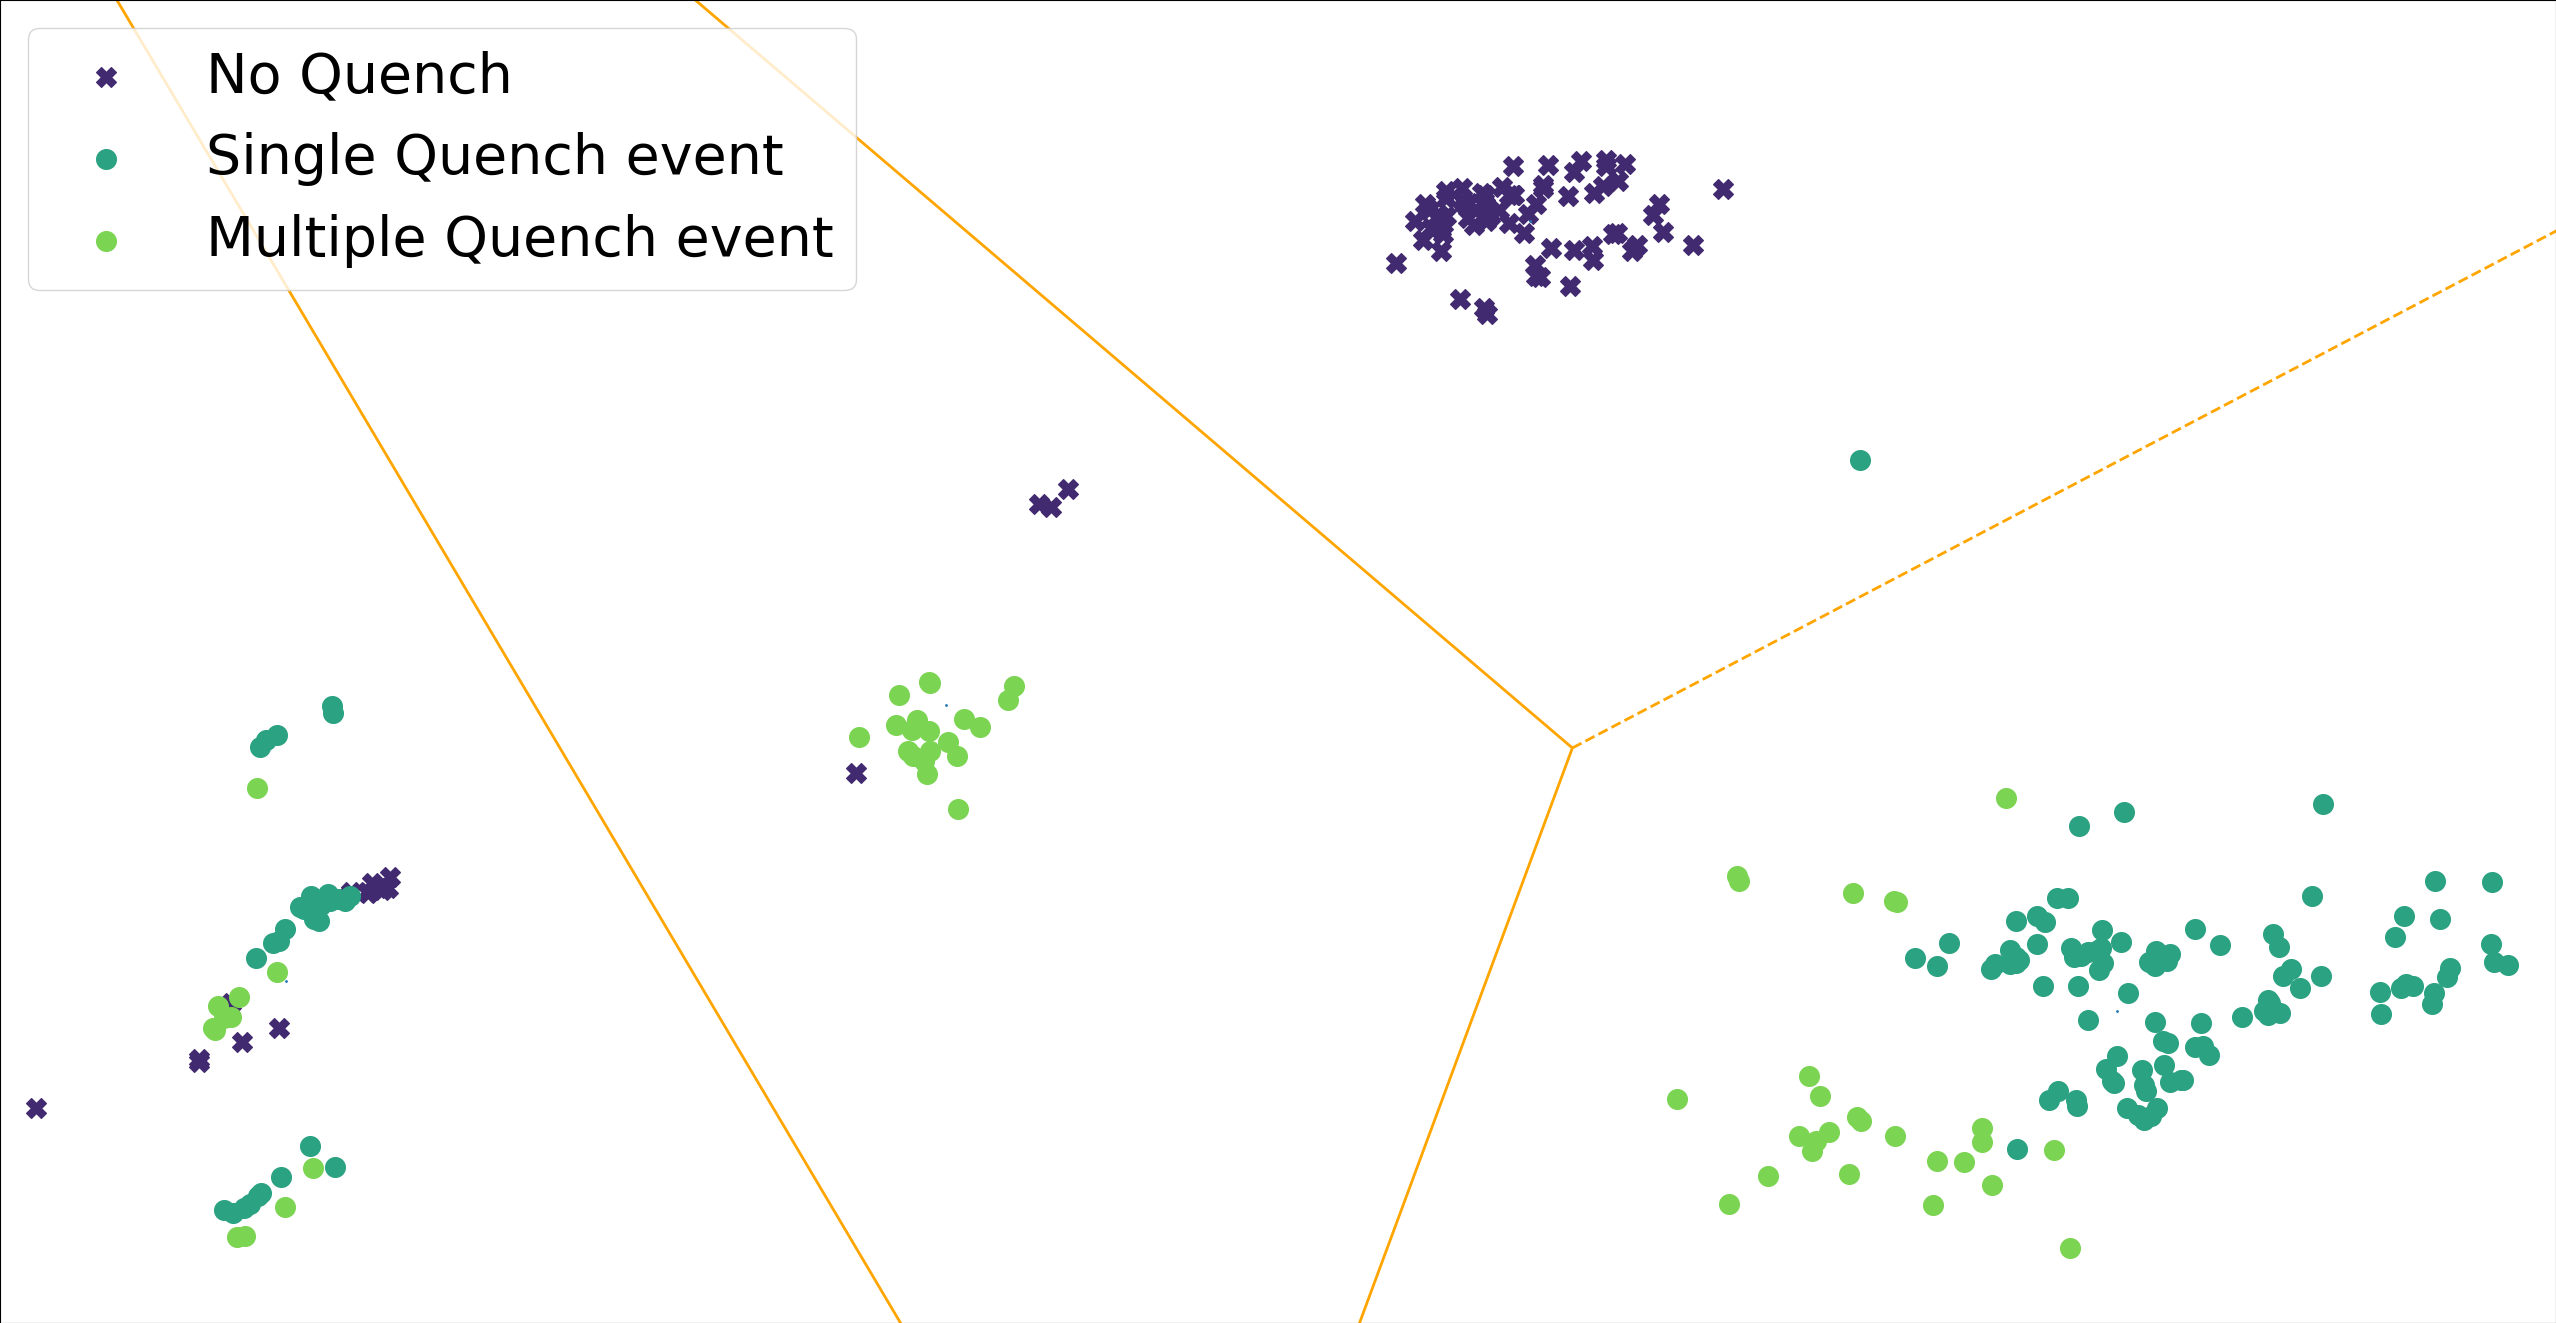
\includegraphics[width=\linewidth]{img/clustering_cnmod_qlp_4c.png}
		\caption{}
	\end{subfigure}
	\caption{} \label{fig:4-means-results}
\end{figure}

Technically, according to the clustering-specific performance metrics that we obtained on the dataset using
$4$ clusters was supposed to yield the best possible performance in both cases and we suppose that,
at least for \cnmod, it could be a good preprocessing step for \qrp. We could then achieve very high
performance with a simple tree classifier built on the cluster(s) with the lowest purity. This
approach, though interesting, would lose the propriety of explainability (since both \pca\ and
$k$-means are unsupervised techniques).

We experimented with higher cluster counts and we discovered that, while the cluster distribution
for \cnmod\ gets worse with the increase, the algorithm finds very well separated clusters with a
high level of purity on \an. \Cref{fig:clustering-an} plots the result of a $8$ cluster $k$-means clustering run. As we can see,
the clusters identified by the algorithm are very clearly trying to separate three classes of
samples: one associated to the magnet being in normal working condition, one associated to the
magnet containing \emph{at most} one quenched coil, and finally, one associated to the magnet
containing \emph{at least} one quenched coil.
\begin{figure}[!ht]
	\centering
	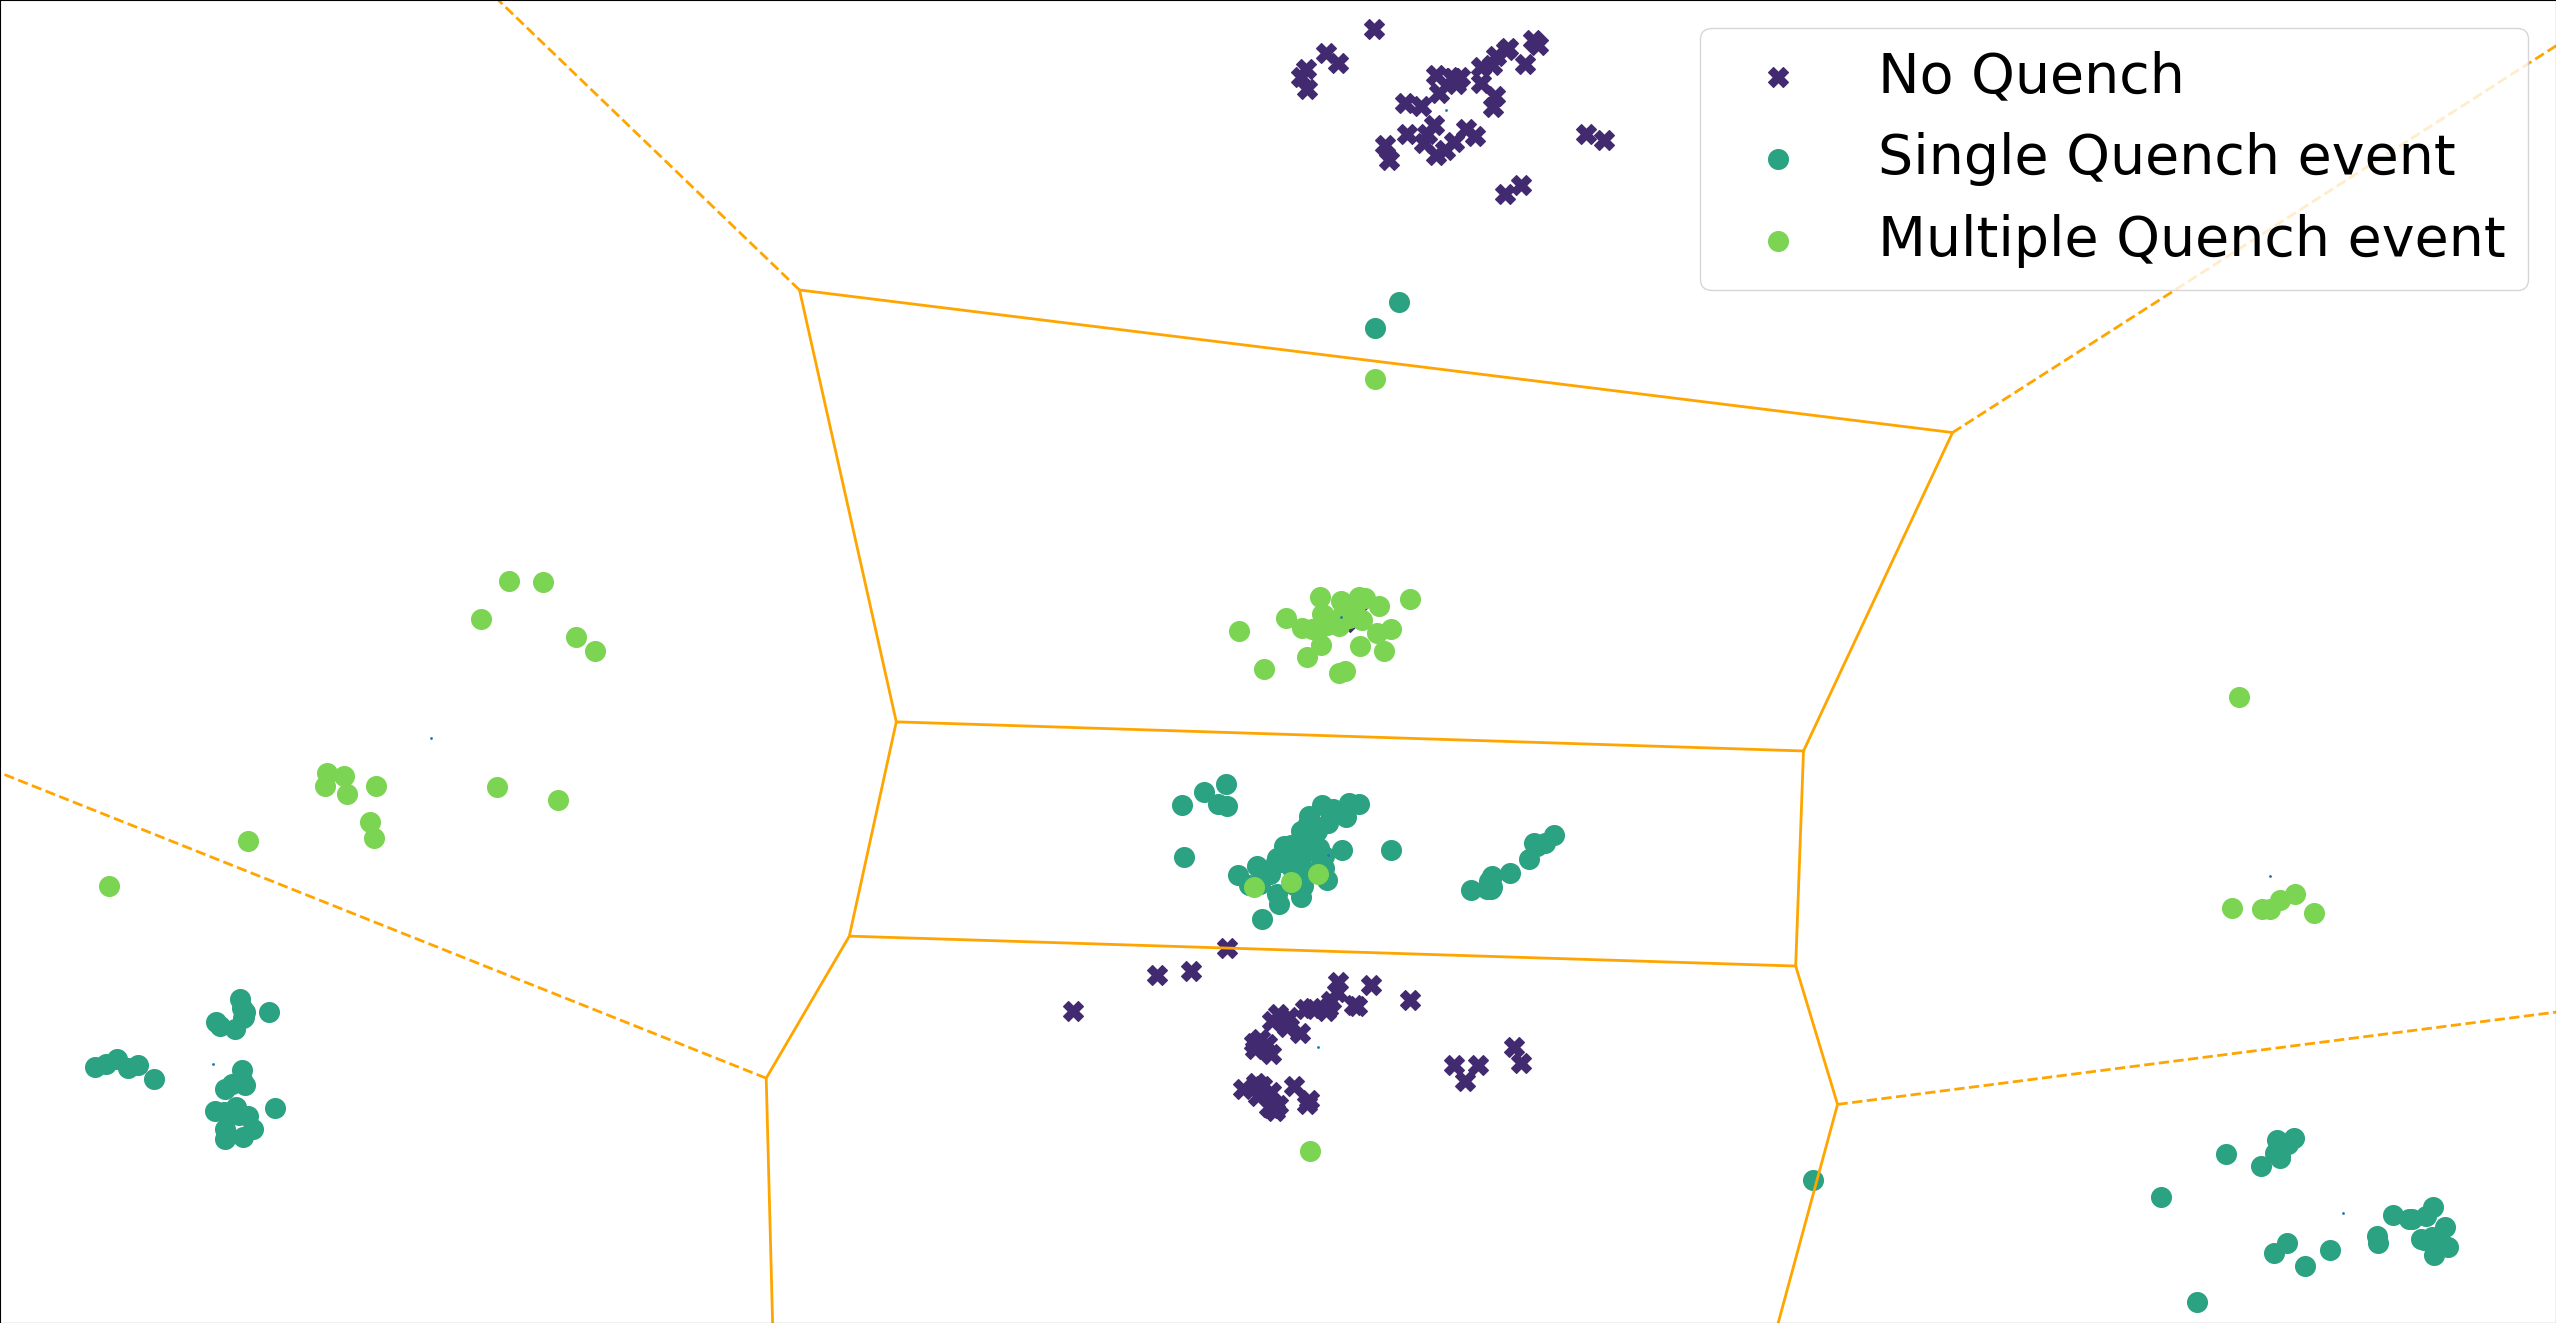
\includegraphics[width=0.8\linewidth]{img/clustering_an_qlp_8c.png}
	\caption{}\label{fig:clustering-an}
\end{figure}
Clustering provided very interesting results, that could be further explored by using diverse
techniques, one example could be to use a supervised clustering algorithm like $k$-nn to correct the
cluster structure computed using $k$-means.

\section{Results}
After our brief exploration of the possibilities offered by clustering algorithms, we moved back to
supervised machine learning algorithms to solve \qlp. Our first approach was to do a na\"ive
extention of the models used to solve \qrp, to the multiclass-classification environment. We didn't
have high expectations for such models since they would have to predict $4$ different bits, instead of just one, making the problem
much more difficult than the original one.

As a matter of fact, trees, which have always been quite easy to interpret, in the case of \qlp\
became much more complicated to read. Even if they always had maximum depth between $5$ and $10$
(therefore having a structure close to the limit of what we would consider explainable) the accuracy
was close to $60 - 70\%$. This rough performance number was obtained by micro averaging the accuracy
for every class, in other words, the resulting metric is the average of the metric computed on each
class weighted on the cardinality of the class.

Since the performance obtained using a direct extension of trees didn't really suit our expectations
we chose to change approach. Our new idea was simply to turn \qlp\ into a problem that could be
solved by simply solving a variation of \qrp\ $4$ different times, one per coil. We solved a
variation of \qrp\ and not \emph{the actual} \qrp, since the relation we originally wanted to find
connected the harmonic decomposition of magnetic field to quench events in a quadrupole. This new
version of \qrp\ requires us to find a function that links \emph{the same data} to a different
value, that states whether coil $i$ quenched or not.

It might sound like a very subtle change, but it's an important one. So much so that, if we tried to
reuse the best models we found for \qrp, to solve \qlp, we wouldn't get similar performance metric.
In the following sections we will retrace our steps in \Cref{chp:qrp} and discuss the obtained
results for the various models.

\subsection{Decision trees}
As we said previously, decision trees utilized in the multiclass-classification environment provided
performance that left a lot to be desired, to counteract this we chose to reinterpret \qlp\ as a
problem in which we need to understand whether each coil has quenched, separately (therefore
solving \qrp\ $4$ different times). To keep the discussion of the performance concise we will be
discussing the structure of the best models and concentrate on the performance of the aggregate.

To evaluate the performance of the aggregate model, containing one classifier per coil, we defined a
metric named 'Hamming score' ($\hs$ in the following), which simply computes how different are the
prediction and the expected outcome.

\Cref{fig:bdts-qlp} contains the performance metrics obtained in the outer \cv\ for the best single
tree trained on each coil. The metrics are quite close to each other, with the only clear outlier
being the model trained on coil $3$.

Instead of including a plot of the various trees we condensed the most important information
in \Cref{tbl:tree-description}, all the trees described have a depth of maximum $5$ and the number
of internal nodes and leaves is always very acceptable, while the trees built on \an\ remain on the
smaller side, the trees built for coil $1$ and $3$ are larger (with the one built on \cnmod\ being
the largest at $15$ total nodes), despite their structure being more complex, these trees struggle
compared to the ones trained on sub-views of \an.

\begin{figure}[!ht]
	\centering
	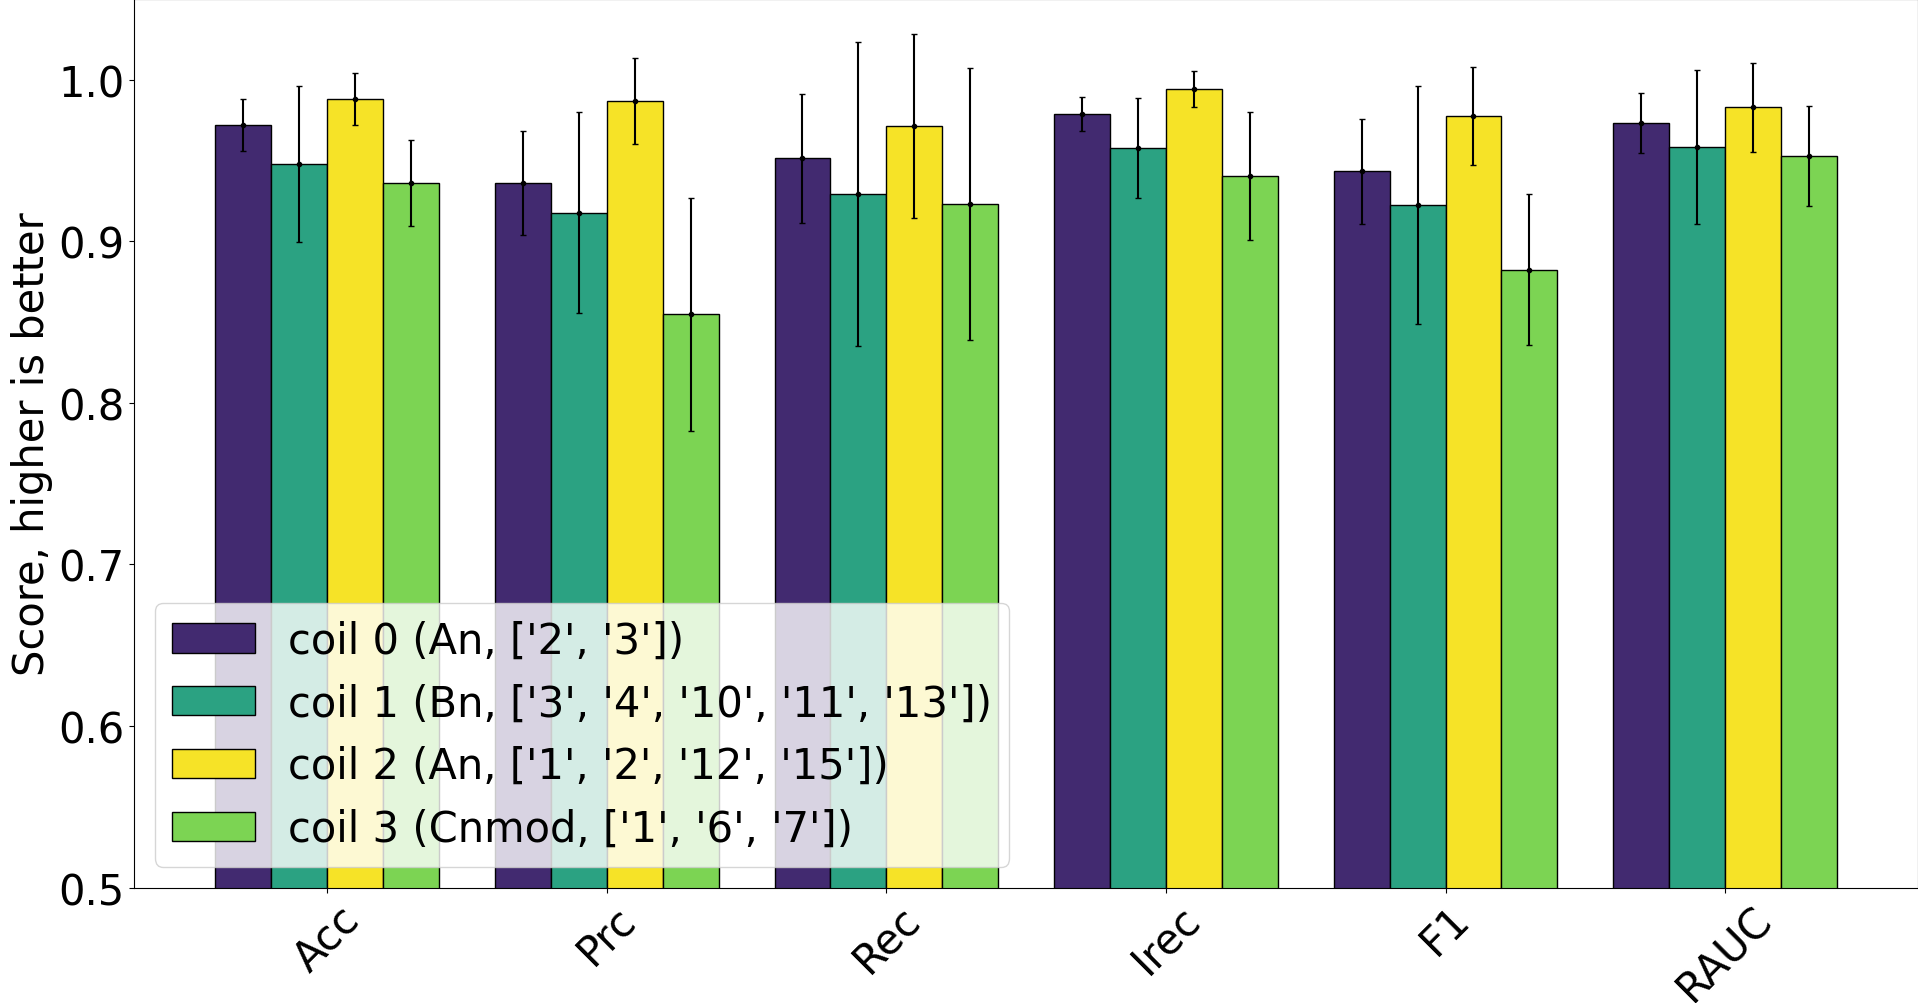
\includegraphics[width=\linewidth]{img/best_dts_qlp.png}
	\caption{Comparing the performance of the best model built on every coil, independently of
		the dataset used.} \label{fig:bdts-qlp}
\end{figure}

\begin{table}[!ht]
	\caption{Description of the best \dt\ for every coil.}\label{tbl:tree-description}

	\bigskip
	\setlength{\tabcolsep}{6pt}
	\centering
	\begin{tabular}{lcccc}
		\toprule
		\textbf{}                           & \textbf{Coil 0}  & \textbf{Coil 1}          & \textbf{Coil 2}          & \textbf{Coil 3}
		\\
		\midrule
		\textsc{attribute}                  & \an              & \bn                      & \an                      & \cnmod                          \\
		\multirow{2}{*}{\textsc{harmonics}} & \an[2], \an[3]   & \bn[3], \bn[4], \bn[10], & \an[1], \an[2], \an[12], & \cnmod[1], \cnmod[6], \cnmod[7] \\
		                                    &
		                                    & \bn[11], \bn[13] & \an[15]                  &                                                            \\
		\textsc{depth}                      & 3                & 5
		                                    & 3                & 5                                                                                     \\
		\textsc{N internal nodes}           & 4                & 5
		                                    & 3                & 8                                                                                     \\
		\textsc{N leaves}                   & 5                & 6
		                                    & 4                & 7                                                                                     \\
		\textsc{N nodes}                    & 9                & 11
		                                    & 7                & 15                                                                                    \\
		\bottomrule
	\end{tabular}
\end{table}

In \Cref{fig:dt-qlp-hs}, we plotted the performance of the aggregate model, which are obtained as we
did when testing \tas\ for \qrp: A run of $5$-fold \cv\ and we computed the number of errors done by
the ensemble on the $4$ bit array. On average the classifiers makes $2$ errors or less, since the
minimum accuracy is $0.5$, averaging the performance of all the folds we get a final Hamming score
which is $0.95$ and with a standard deviation of $0.024$. Testing the performance of the aggregate
on the final blind-test, if we average the Hamming score on the $29$ samples, we get higher
performance on average $0.966$ and a higher standard deviation $0.086$ (this difference is probably
due to the lower amount of data we are averaging on), the trained aggregate makes $4$ single errors
on the $116$ total labels that it needs to predict.

Our supposition at the moment is that finding a better model for coil $3$ would make the performance of
the ensemble better because, while we have been saying that the model is an aggregate of trees, no
aggregation is happening (like in the case of \tas) apart from inserting the predicted bits in a
prediction array, therefore the sub-models are not helping each other and 'covering for each other'.

\begin{figure}[!ht]
	\centering
	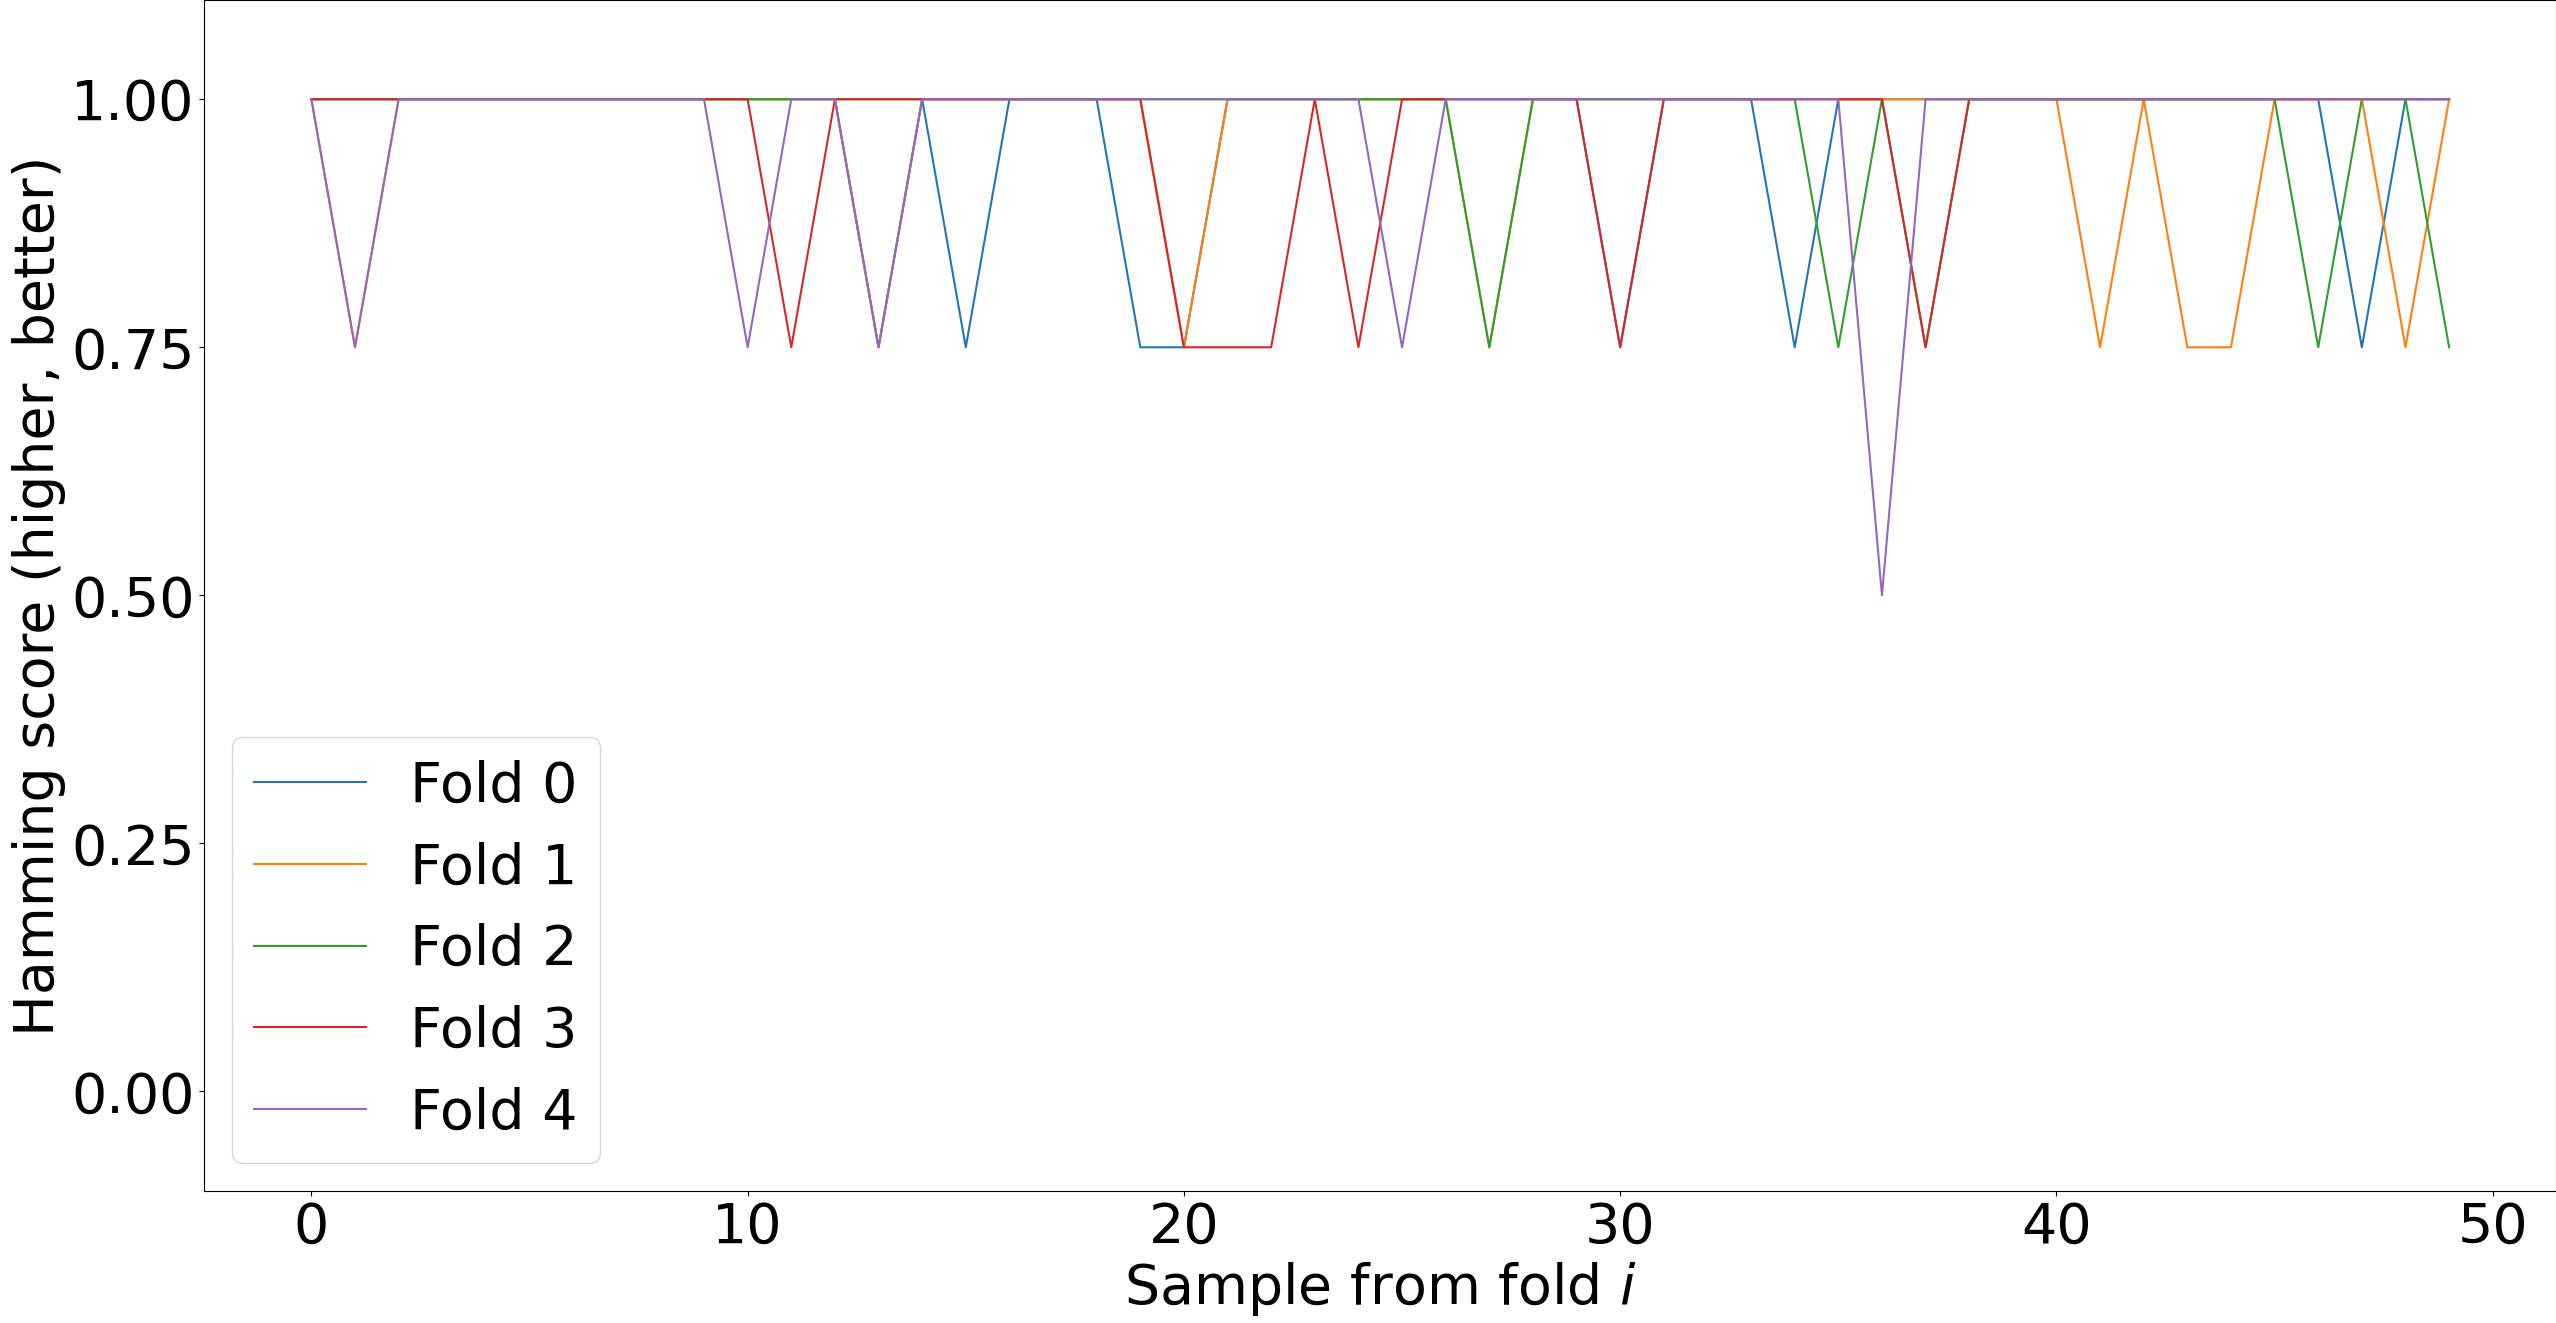
\includegraphics[width=\linewidth]{img/best_dts_hs.png}
	\caption{The Hamming score computed on every fold (for the $50$ samples therein contained), the lower reaching is the line the lower is going to be the accuracy.} \label{fig:dt-qlp-hs}
\end{figure}

\subsection{Random forests}
Similarly to what we just did for \dts\ we also evaluated the performance of a model containing one
single forest per coil, we expected higher performance compared to the ones just obtained on \dts,
at the expense of a lower explainability.

\Cref{fig:brfs-qlp} shows the performance for the best rfs built on a mix of different attributes
(each taken in its entirety), as we can see the performance metrics are better, but we are not far
off from the numbers obtained in the case of \dts\ (see \Cref{fig:bdts-qlp}), also, our weakest
learner, the one built for coil $3$ is not much worse than the proposed random forest, while being
much simpler than the alternative.
\begin{figure}
	\centering
	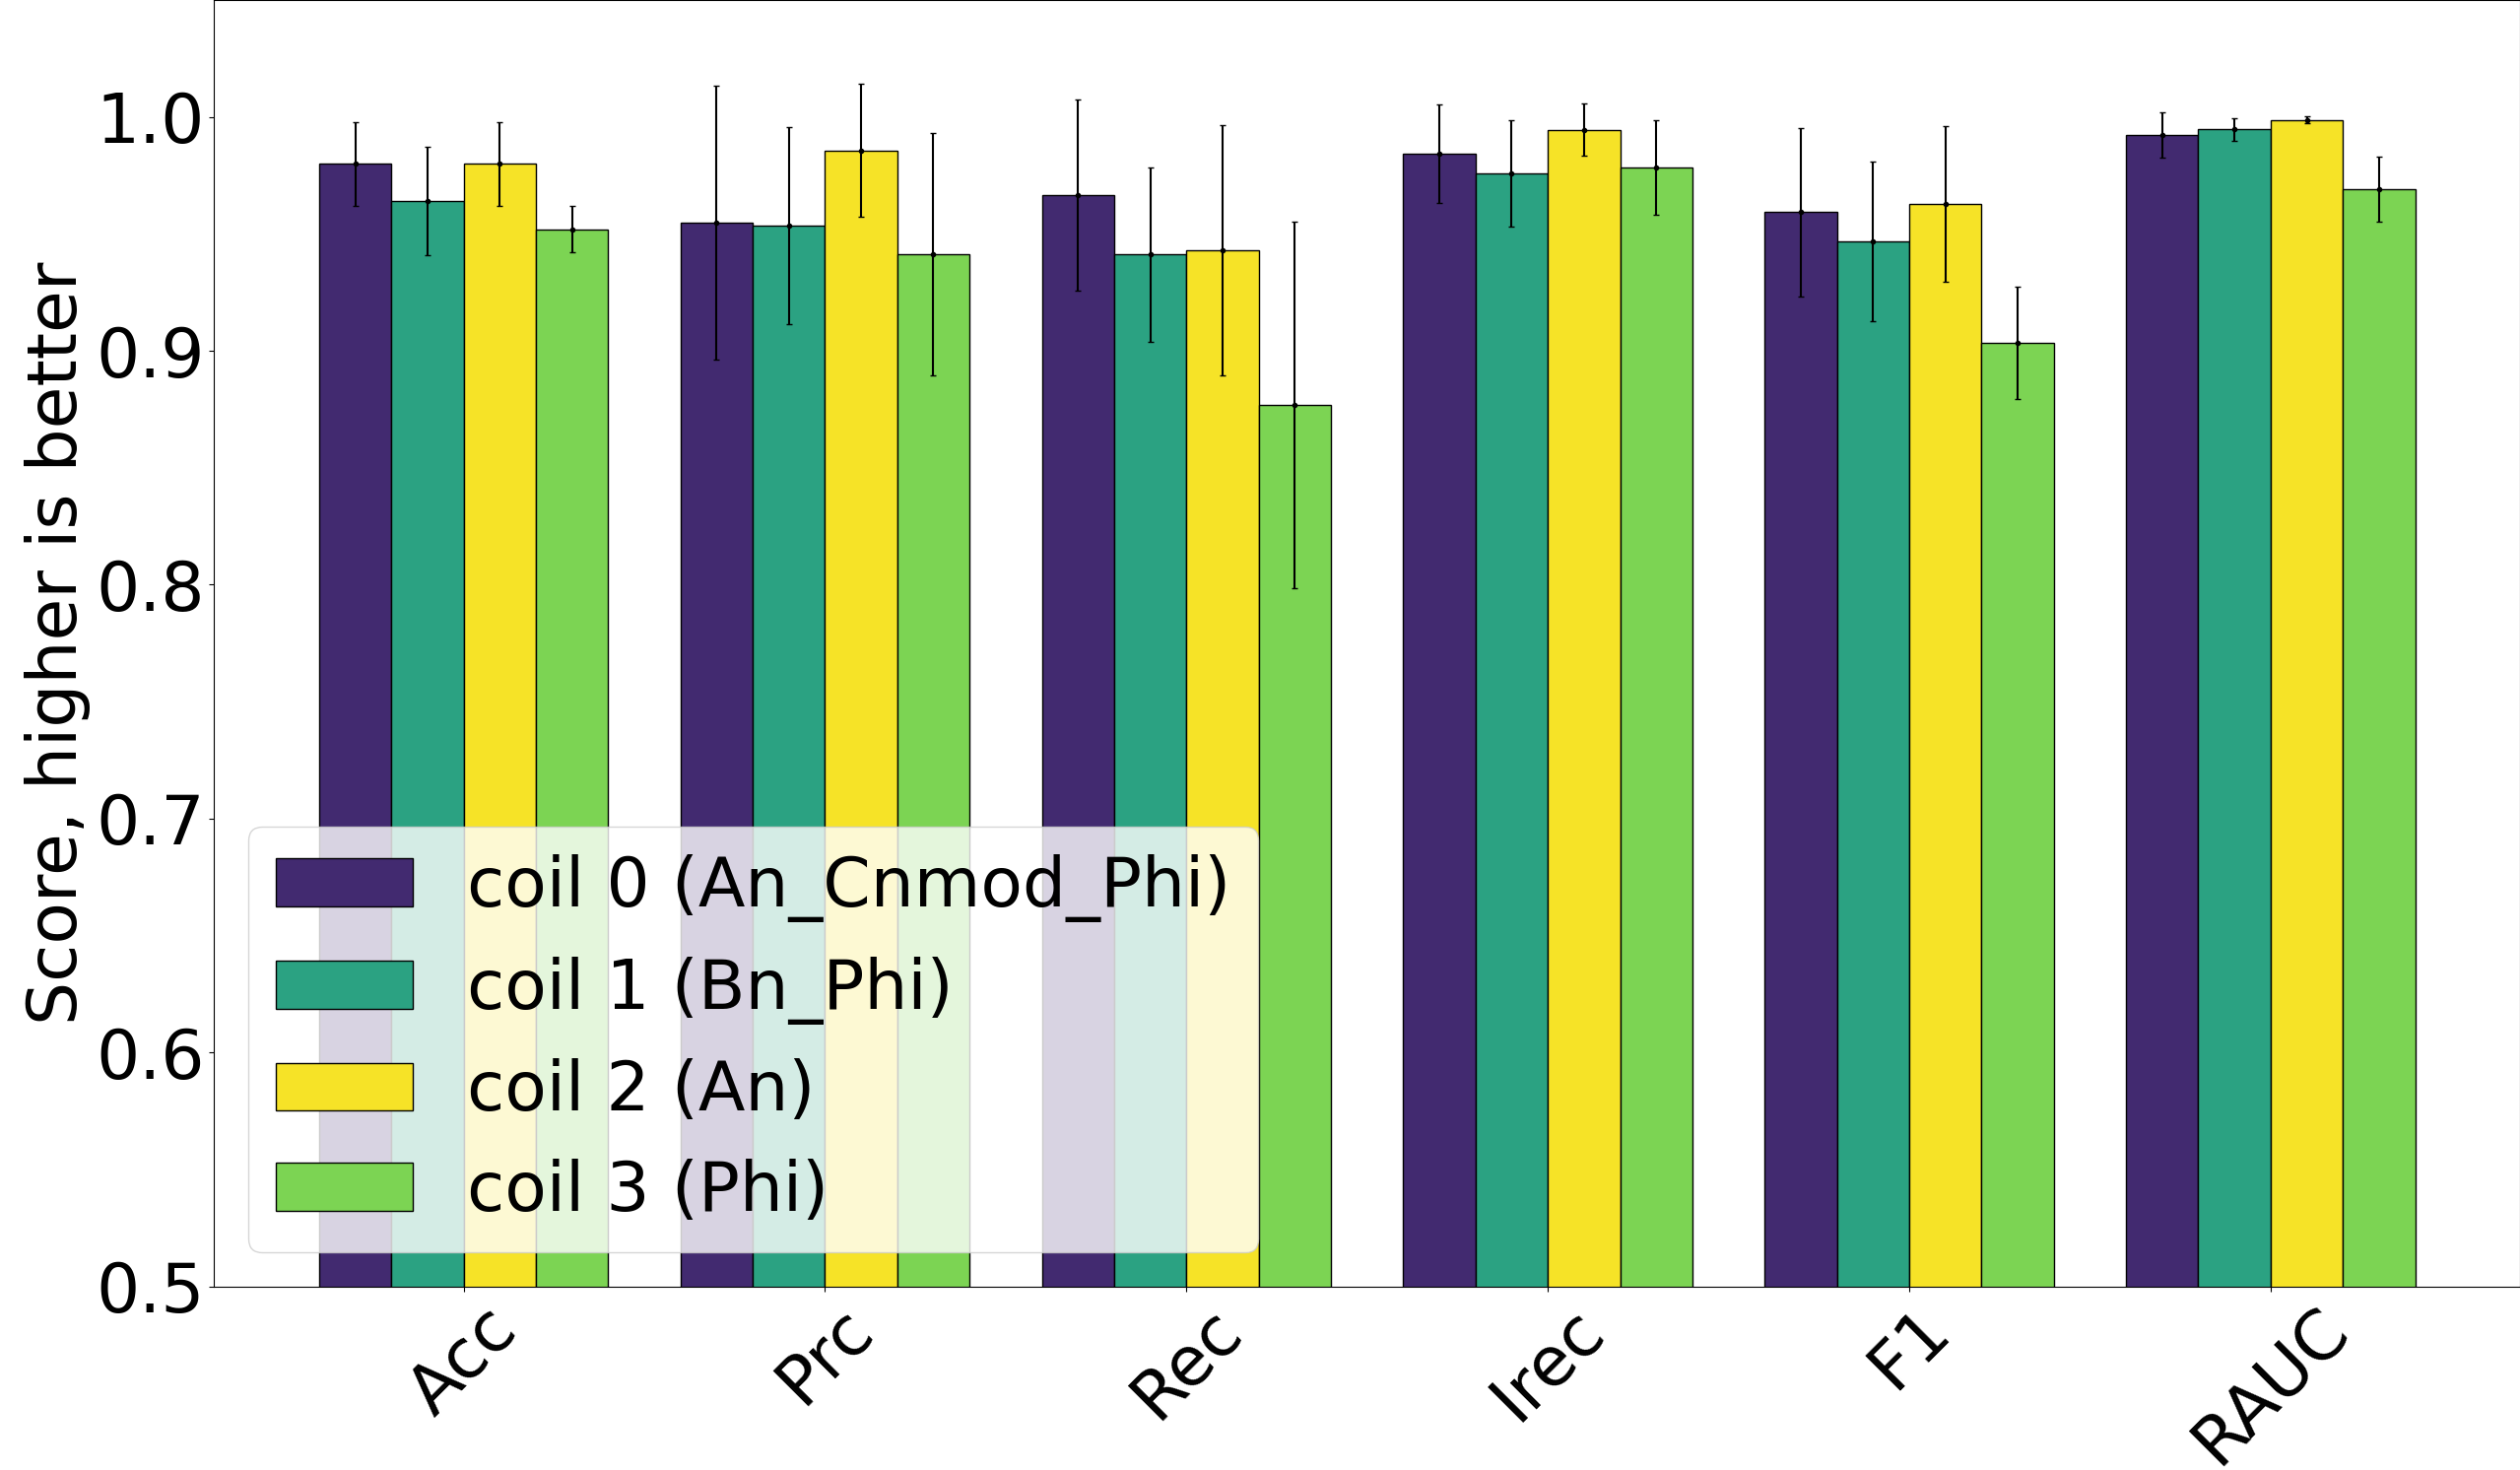
\includegraphics[width=\linewidth]{img/best_rfs_qlp.png}
	\caption{The best random forest trained on a sub-view or mix of sub-views, for every coil,
		since all of the models have been plotted without indicating the harmonic content it means
		that they are using full attributes.}\label{fig:brfs-qlp}
\end{figure}
The \rfs\ in figure contain respectively $5, 10, 10$ and $10$ trees. As we have already said
previously, while trees have a high level of explainablilty, trying to interpret a structure
containing $10$ of them is certaintly a complex task, and I would consider it explainable only on
paper. This is why, for all intents and pourposes, while we provide the results for the Hamming
score in the following, we decided to not follow this lead too much, since it would mean having an
excessive amount of models to consider at the same time.

While the trees for the first three forests are, overall, quite simple (not too deep), contained in
the number of leaves and nodes, the last forest contains complex trees with many layers ($4$ on
average), many internal nodes and leaves. Seeing the complexity of this last tree it's evident that
the forest approach would not be feasible even in an hybrid approach based on both three trees for
the first three coils and an \rf\ for the last one.

Since \rfs\ are more complicated than we would like we avoided the calculation of the Hamming
score, also because the performance are good but not good enough to make us consider their use when
compared to the simpler \dts.

\subsubsection{Support Vector Classifiers}
If we analyze the benchmark model, and we train it without constraints (one or more sub-views for
different datasets), the results are that we can aim at a very high level of performance if we
forget about explainability. Performance have been plotted in \Cref{fig:bsvcs-qlp}, the metrics were
taken from the outer \cv\ loop and the models chosen were the best for each specific coil.
\begin{figure}[!ht]
	\centering
	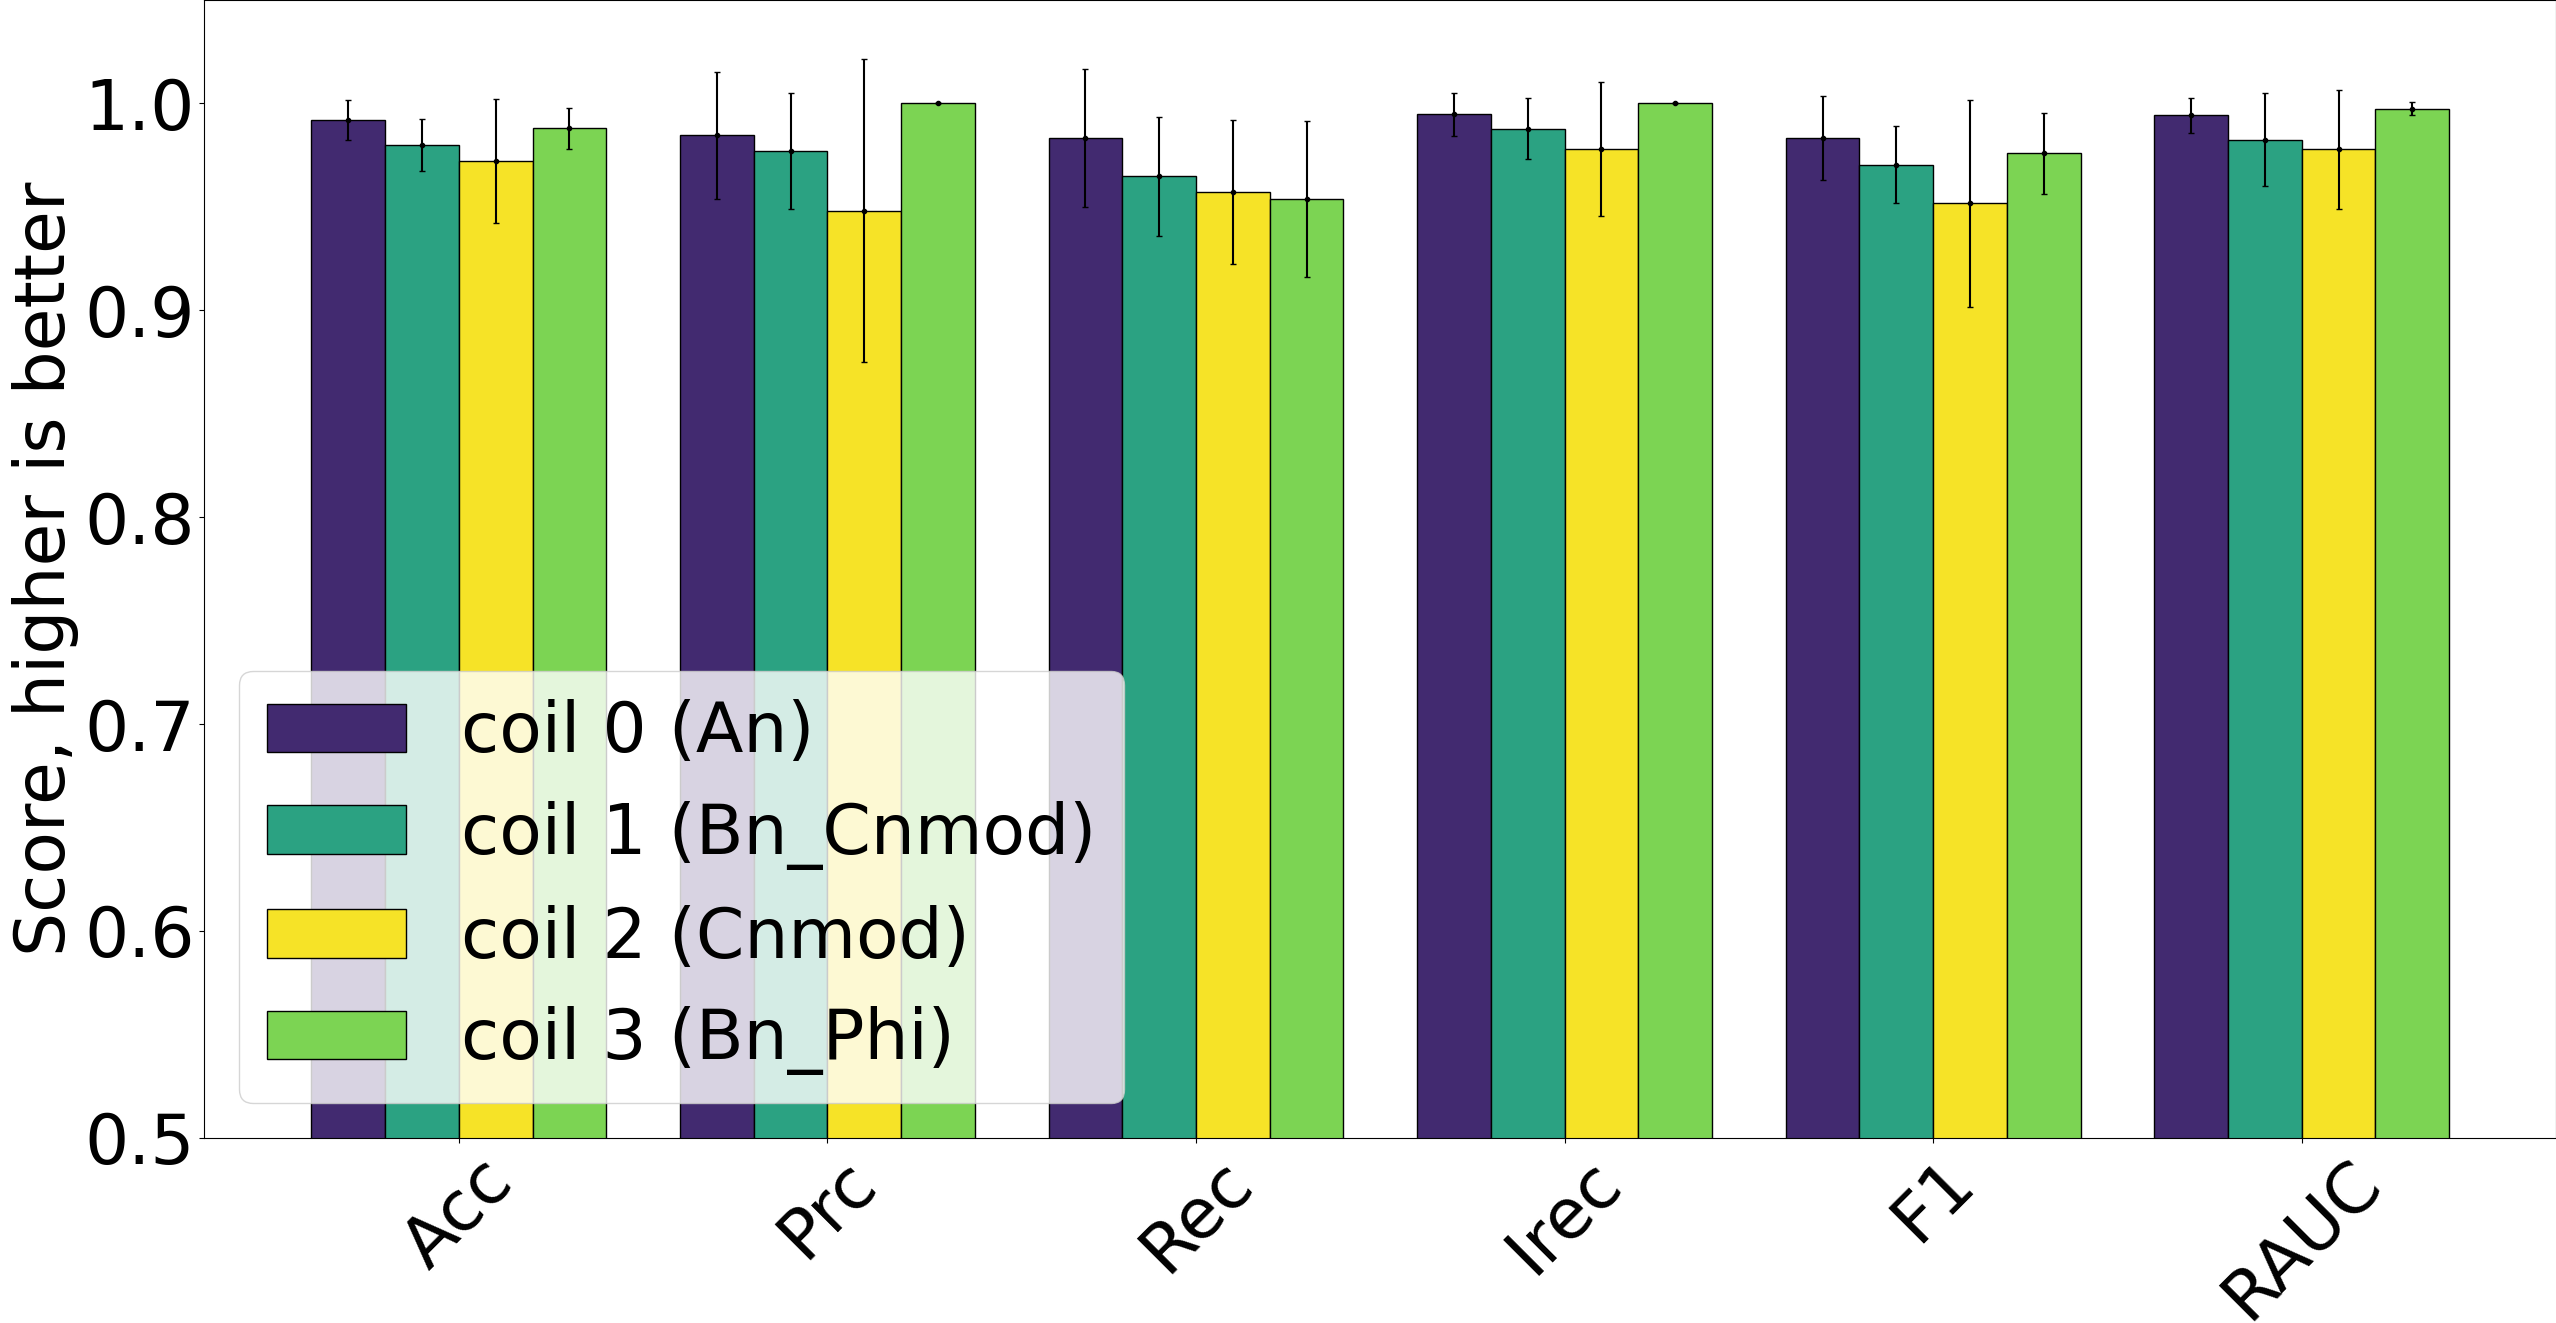
\includegraphics[width=\textwidth]{img/best_svcs_qlp.png}
	\caption{Performance metrics for the best \svcs\ trained on every coil, all attributes
		have been taken with their full harmonic content.} \label{fig:bsvcs-qlp}
\end{figure}
There are a couple of very interesting takeaways:
\begin{itemize}
	\item The best \svc\ trained on coil $0$ is based on attribute \an. This is exactly what we
	      expected since the very beginning of this chapter.
	\item The best models for coils $1$ and $3$, were trained on \bn\ and another dataset (\cnmod\ for $1$
	      and \phin\ for $3$). This is interesting for two reasons:
	      \begin{inparaenum}[(i)]
		      \item \bn\ is actually the best attribute for the two coils, as we saw in the analysis
		      we did in the beginning of the chapter,
		      \item the \svc\ trained on the sole \bn\ performed worse than the alternatives. This
		      lead us to believe that, like in the case of \qrp, \bn\ alone doesn't contain
		      enough information
	      \end{inparaenum}.
	\item Interestingly, while \cnmod\ didn't perform well enough in our tests on trees for coil
	      $2$, in the case of \svc\ the model was picked over \an.
\end{itemize}
Evidently, the ceiling of performance is still very high, and we can still find ways to get closer
to the performance of our benchmark model.








